% ####################################################################

\setcounter{chapter}{2}
\chapter{Baseline experiments}
\label{c:base}

The grammatical square\is{grammatical square} (see Figure \ref{f:stage4}) illustrates the multifunctional and indirect nature of case marking\is{case!case marking}. It can also be read as a `research roadmap' for experiments on the emergence\is{formation} of a grammar for case. More specifically, the experiments must investigate how a population\is{speech population} of agents can evolve a grammar which takes care of (1) the mapping between event-specific participant role\is{participant role}s and generalized semantic role\is{semantic role}s, (2) the mapping between semantic role\is{semantic role}s and grammatical cases, and (3) the mapping between cases and surface case marker\is{case!case marking}s. Constructing and aligning this kind of grammar in a multi-agent population\is{speech population} is incredibly difficult because all mappings are agent-internal and are thus not directly observable by other agents. Moreover, these mappings vary depending on the communicative and linguistic context so the agents have to be capable of dealing with polysemy\is{polysemy}. Finally, linguistic convention\is{convention}s may constantly change so the agents have to be able to adapt to newly propagat\is{propagation}ed constructions.

In this Chapter I will present three baseline experiments which first replicate simulations reported by \citet{steels02simulating, steels04constructivist} and then lift them towards a multi-agent simulation. I will specifically focus on which diagnostic\is{learning strategies!diagnostics}s, repair\is{learning strategies!repair strategies}s and alignment strateg\is{alignment strategy}ies are needed for each step of increased complexity. In the next section, I will first give an overview of the experimental set-up that is shared by all experiments after which the simulations themselves are reported.

\section{Experimental set-up}

\begin{table}[t]
% \centerline{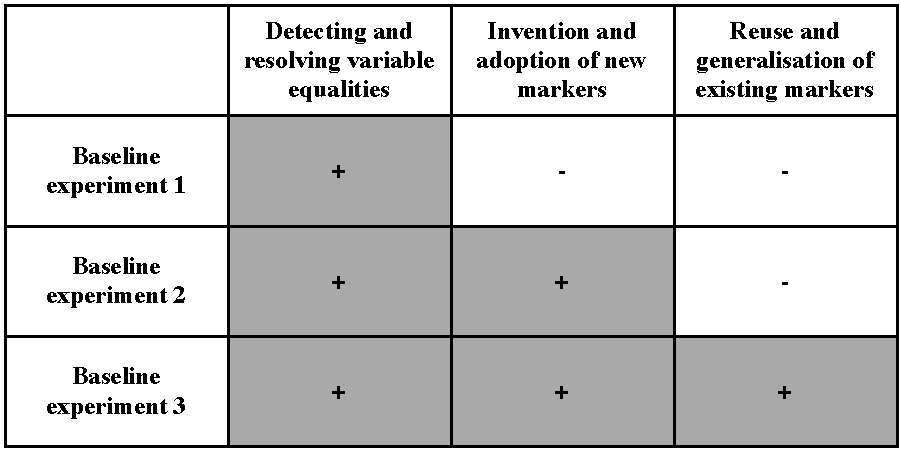
\includegraphics[width=\linewidth]{Chapter3/figs/repairs}}

\begin{tabular}[c]{p{2.5cm}ccc}
 \lsptoprule
 & \parbox{3cm}{\raggedright Detecting and resolving variable equalities} 
	&\parbox{2.5cm}{\raggedright Invention and adoption of new markers}
		&\parbox{3cm}{\raggedright Reuse and generalisation of existing markers} \\
		\midrule
\raggedright Baseline experiment 1 & \cellcolor[gray]{0.9}\raisebox{-.5\height}{$+$}& \raisebox{-.5\height}{$-$} &\raisebox{-.5\height}{$-$} \\
\raggedright Baseline experiment 2 & \cellcolor[gray]{0.9}\raisebox{-.5\height}{$+$}& \cellcolor[gray]{0.9}\raisebox{-.5\height}{$+$} &\raisebox{-.5\height}{$-$} \\
\raggedright Baseline experiment 3 & \cellcolor[gray]{0.9}\raisebox{-.5\height}{$+$} & \cellcolor[gray]{0.9}\raisebox{-.5\height}{$+$} &\cellcolor[gray]{0.9}\raisebox{-.5\height}{$+$}\\
 \lspbottomrule
\end{tabular}



\caption[Key cognitive abilities in the baseline experiments]{This table shows the key cognitive abilities which are given to the agents in the baseline experiments. In the first experiment, agents are `intelligent' enough to resolve variable equal\is{variable equality}ities by using their world model but they cannot express these equal\is{variable equality}ities in their language. In experiment 2, the agents can decide to invent new marker\is{case!case marking}s to indicate the linking of equal\is{variable equality} variables but they cannot generalize or abstract. In the third experiment, the agents can perform analog\is{analogy}ical reasoning over event structure\is{event structure}s to generalize existing marker\is{case!case marking}s.}
\label{t:repairs}
\end{table}

The simulations in this book investigate how a population\is{speech population} of artificial agents can autonomously construct a shared grammatical system for marking event structure\is{event structure} (in the form of a case grammar\is{case!case grammar}). As argued in section \ref{s:methodology}, we need to hypothesize which cognitive mechanisms and external pressures are the minimal ingredients that enable the agents to do so, and we need to operationalize them into computational processes and a world environment. Since case marking\is{case!case marking} is a complex phenomenon, I will divide the topic into several subparts that follow the stages of development identified in section \ref{s:case-markers}.

\subsection{Key abilities and self-assessment criteria}

In the problem-solving\is{problem-solving} approach adopted in this book, innovat\is{innovation}ion and language change\is{language change} happens in three steps: (1) the speaker innovat\is{innovation}es and is therefore the main cause of potential language change\is{language change}, (2) the hearer tries to infer and learn the innovat\is{innovation}ion through an `abductive process' (as opposed to uniquely relying on inducti\is{induction}on or genetically evolved innate knowledge), and (3) the innovat\is{innovation}ion propagat\is{propagation}es in the population\is{speech population}. Step (1) may be skipped when the hearer overgeneralizes or imposes more systematicity\is{systematicity} on the utterance than introduced by the speaker. Hearer-based innovat\is{innovation}ion or `reanalysis\is{reanalysis}' can be described in terms of the same cognitive processes as involved in speaker-based innovat\is{innovation}ion so the two sources of innovat\is{innovation}ion are complementary to each other \citep{hoefler08reanalysis}. Step (3) implies that an innovat\is{innovation}ion only becomes a linguistic convention\is{convention} if it has been adopted by a sufficient number of language users. Propagation is made possible through the alignment strateg\is{alignment strategy}ies of the agents.

This approach requires a population\is{speech population} of agents endowed with rich cognitive capabilities. As argued in section \ref{s:methodology}, agents can only make use of local measure\is{measure!local measure}s such as communicative success\is{communicative success} and cognitive effort\is{cognitive effort} for steering their linguistic behaviour. The cognitive mechanisms of the agents therefore have to enable the agents to move into a meta-level in which they can {\bfseries self-assess\is{self-assessment}} what problems they encounter during communication, whether there is opportunity for optimization, or what the reasons for success and failure are in a language game\is{language game}. They need to be able to couple this {\bfseries diagnosis} to {\bfseries repair\is{learning strategies!repair strategies} strategies} in order to solve their communicative problems and to their {\bfseries alignment strateg\is{alignment strategy}ies} in order to converge on a shared language. All the experiments in this book mainly focus on the effect of these three aspects: diagnostic\is{learning strategies!diagnostics}s, repair\is{learning strategies!repair strategies}s, and alignment strateg\is{alignment strategy}ies.

The baseline experiments reported in this Chapter first of all replicate the two-agent simulations reported by \citet{steels02simulating, steels04constructivist}. These experiments only focus on the first three stages of case marker\is{case!case marking} development ranging from no marking to the formation\is{formation} and marking of semantic role\is{semantic role}s. Additionally, the experiments are pushed forward to multi-agent simulations in which language convergence becomes the main issue. All three baseline experiments share the same world environment, communicative task, and assumption\is{assumption}s and scaffold\is{scaffold}s (see below). However, they differ in the {\bfseries key cognitive abilities} that the agents are endowed with. I define `key cognitive abilities' as those mechanisms that are hypothesized to be crucial for the transition in the grammar from one stage to the next, and of which the simulations need to demonstrate or falsify whether this is indeed the case. Table \ref{t:repairs} illustrates the difference between the baseline experiments in terms of key cognitive abilities and can be summarized as follows:

\begin{enumerate}
\item In baseline experiment 1 (corresponding to stage 1 -- section \ref{s:stage1}), agents are given the diagnostic\is{learning strategies!diagnostics} to figure out how the meanings of lexical items are linked to each other by exploiting the situatedness\is{situatedness} of the interaction. However, the agents have no means of exten\is{extension}ding their language to explicitly mark the relations between words;
\item In baseline experiment 2 (corresponding to stage 2 -- section \ref{s:stage2}), agents are endowed with a repair\is{learning strategies!repair strategies} strategy which enables them to invent a participant role\is{participant role}-specific case marker\is{case!case marking} for optimizing communication;
\item In baseline experiment 3 (corresponding to stage 3 -- section \ref{s:stage3}), agents are endowed with the capacity to perform analog\is{analogy}ical reasoning over event structure\is{event structure}s. They can exploit this capacity for generalizing existing marker\is{case!case marking}s to cover new participant role\is{participant role}s. As I will show later, generalization is not a goal in itself but rather a side-effect of the need for optimizing communication.
\end{enumerate}

These key cognitive abilities will be explained in more detailed along with the experiments further down in this Chapter. The abilities are each time given and fixed by the experimenter and the simulations do not explain where they come from. However, the global vision underlying this work is that speakers and hearers can autonomously configure their language capacity by recruiting cognitive mechanisms that are also used for other tasks such as hierarchy\is{hierarchy} building operators \citep{steels07recruitment}. This process is driven by needs in communicative success\is{communicative success}, expressive power and the convention\is{convention}s adopted by other agents in the population\is{speech population}. Here again, agents have to be capable of self-assess\is{self-assessment}ing when to recruit a mechanism, which ones are the best candidates, and to self-regulate the semantic complexity of their communication. For simulations that investigate self-regulation and reconfiguration of the language faculty\is{language faculty} on the longer run, see \citet{steels06how-grammar, steels07scaffolding}. In the remainder of this section, I will describe those aspects of the simulations which are shared by all the experiments.

\subsection{Description games}

\begin{figure}[t]
\centerline{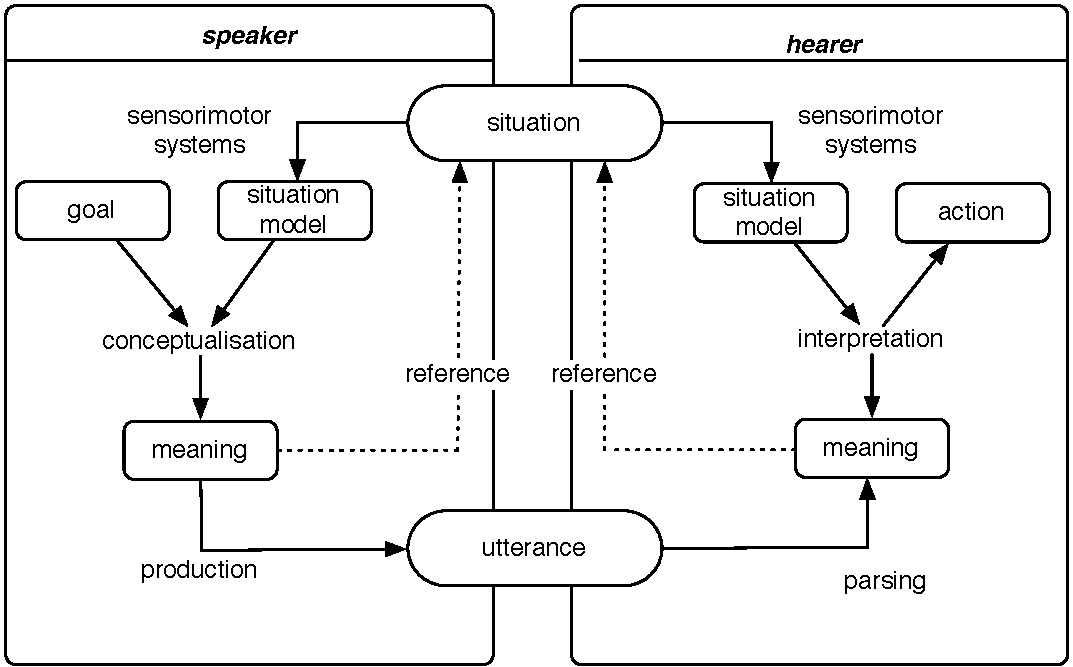
\includegraphics[width=0.8\linewidth]{Chapter3/figs/cycle}}
  \caption[The semiotic cycle]{The semiotic cycle\is{semiotic cycle} involved in language game\is{language game}s. There are three systems working in tight interaction with each other: the sensory-motor system\is{sensory-motor system} (perception and modeling), the conceptual/intentional system\is{conceptual/intentional system} (conceptualization\is{conceptualization} and interpretation), and the linguistic system (production and parsing). This book mainly focuses on the latter one and is complementary to other research efforts on grounded language use and conceptualization\is{conceptualization}.}
   \label{f:cycle}
\end{figure}

An obvious requirement for developing a grammar for marking event structure\is{event structure} is {\bfseries communication about events}. This is operationalized in the form of the {\bfseries description game\is{language game!description game}}, a routinized communicative interaction which involves the complete semiotic cycle\is{semiotic cycle} as illustrated in Figure \ref{f:cycle}. Applied to the simulations in this book, the interaction pattern conforms to the following script:

\begin{enumerate}
\item Two agents are randomly selected from the population\is{speech population}. One will act as speaker, the other as hearer. The speaker and hearer start a {\bfseries local language game\is{language game}} so the other agents cannot observe it;
\item {\bfseries Joint attention\is{joint attention}} \citep{tomasello95jointattention} between the agents is required and assumed. This is operationalized by giving the agents a shared context. The context contains one or more events (depending on the complexity of the game) which are observed by the agents;
\item Both the speaker and the hearer build a {\bfseries world model} based on the observed events. The world model consists of a series of facts in the memory;
\item The speaker is given a communicative goal. In this book, the goal is always to {\bfseries make an assertion} about a certain state of affairs in the context (i.e. the speaker has to describe an event);
\item The speaker chooses an event to describe and {\bfseries conceptualizes} a meaning for it. Conceptualization involves profiling\is{event profile} of the event and finding a discriminating meaning for the participants in the event (see further below);
\item The speaker then verb\is{verb}alizes the meaning by {\bfseries producing} an utterance which is transmitted to the hearer;
\item The hearer observes the utterance and {\bfseries parses} it;
\item The hearer then {\bfseries interprets} the parsed meaning by comparing it to the facts in the world model. This leads to the {\bfseries mental action} of agreeing or disagreeing with the description;
\item The hearer signals agreement with the description if the parsed meaning is unambiguously compatible with the hearer's world model, or signals disagreement if it is not. Agreement means {\bfseries communicative success\is{communicative success}}, disagreement means {\bfseries communicative failure}. No other kinds of feedback or requests for information are included;
\item Based on the outcome of the game, both agents {\bfseries consolidate} their linguistic inventor\is{linguistic inventory}ies. 
\end{enumerate}

\subsection{The world, sensory-motor input and conceptualization}
\label{s:world}

\begin{figure}[t]
\centerline{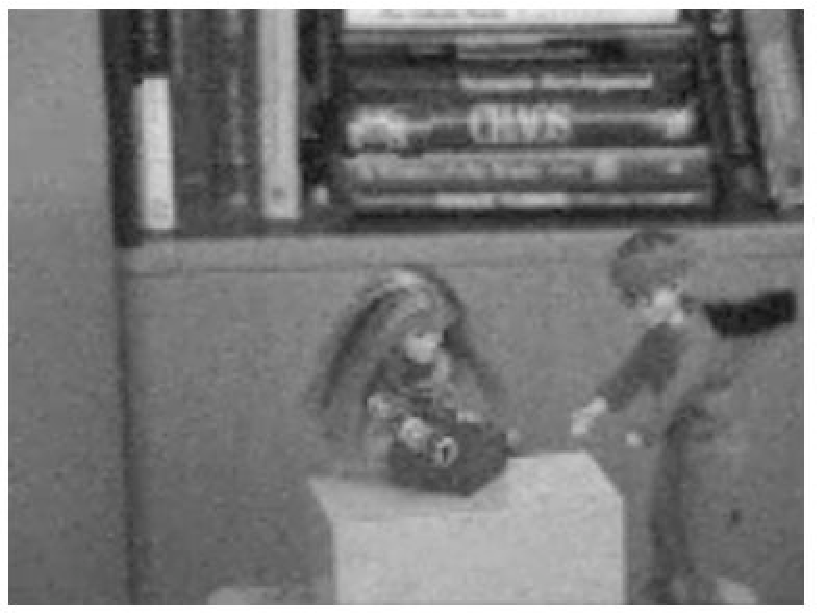
\includegraphics[width=0.65\linewidth]{Chapter3/figs/puppets}}
  \caption[An example scene]{The world environment consists of dynamic scenes in which puppets perform various actions such as walking and pushing blocks to each other. Here, one puppet `gives' a block to another puppet by sliding it over a table. The scene contains four participants (two puppets, a block and a table), a `ground' and various micro- and macro-events.}
   \label{f:puppets}
\end{figure}

The semiotic cycle\is{semiotic cycle} in Figure \ref{f:cycle} clearly shows that linguistic processing is only one part of the general cognitive architecture which is involved in communication. Even though the experiments in this book mainly focus on the production and parsing of linguistic utterances, at least two other systems are directly relevant for communication: the sensory-motor system\is{sensory-motor system} (in a broad sense responsible for dealing with the sensory experience and for building a world model) and the conceptual-intentional system (responsible for conceptualization\is{conceptualization} and interpretation as well as concept\is{concept formation} formation\is{formation}). These three `systems' work together in tight interaction and without a clear-cut division between them.

In this section, I will describe what kind of world environment is used in the experiments, what kind of world model is built by the sensory-motor system\is{sensory-motor system}, and what kind of meanings are conceptualized for communication. These three elements remain constant and are shared by all the experiments.


\subsubsection{The environment}
 The environment in the experiments consists of dynamic real-world scenes from a small puppet theater. The puppets perform various actions such as moving, disappearing from a scene, walking towards each other, and carrying objects. The use of real-world scenes is part of earlier work on grounded language communication \citep{steels02simulating, steels03shared} and is not essential to the dynamics of the models reported in this book: a simulated world suffices for the scope of this book and can in fact be used for scaling up the experiments to larger worlds. The choice for using data from real-world scenes was made in order to demonstrate that the models {\em can} be incorporated into research on the grounding of communication.

For the baseline experiments, 20 different scenes were recorded comprising 207 event token\is{event token}s belonging to 15 different event types. There are 103 event token\is{event token}s which take one participant (e.g. a `move-event'), 99 event token\is{event token}s which potentially take two participants (e.g. a `walk-to'-event) and 5 event token\is{event token}s which potentially involve three participants (e.g. a `give-event'). Given the conceptualization\is{conceptualization} algorithm (see below), this leads to a frequency\is{frequency} of about 64\% of utterances involving one participant, about 34\% of utterances involving two participants and only 2\% of utterances involving three participants. In most experiments each event type\is{event type} was given the same frequency\is{frequency} in order to balance this skewed frequency\is{frequency}. As I will demonstrate later, equal\is{variable equality} frequency\is{frequency} offers a much clearer picture of the propagat\is{propagation}ion and convergence dynamics in the experiments.


\subsubsection{Sensory-motor input}
 The real-world scenes were recorded using two SONY pan-tilt cameras (EVI-D31) which were hooked up to computers running the PERACT\is{PERACT system} system \citep{baillie00action, steels03shared}, which was designed for the visual recognition of events and which is related to other attempts in visual-recognition such as \citet{siskind00visual}. Even though two cameras were used, this book uses only the data obtained through one of them. The simulations are thus not affected by differences in world models due to noisy recognition of the events or differences in visual perspective. These difficulties are very interesting for investigating the robustness of the model in grounded communication, but are not part of this book.

Since the vision system is quite complex (but fortunately well-documented in \citealp{baillie00action}), I will restrict my discussion to its general architecture and to the design choices that are important for understanding what information is delivered to the language system. The PERACT\is{PERACT system} system first delineates objects based on colour\is{colour} histograms and then groups the pixels belonging to the same object together. These objects (two puppets, a table, two blocks, etc.) were learned in advance and PERACT\is{PERACT system} can handle seven of them simultaneously in one scene. Starting from basic visual `primitives' or `micro-events' such as touching, movement and appearance, the system tracks the objects in real-time and assembles more complex descriptions (or `macro-events') when it recognizes a pattern in the scene. This recognition is often unreliable, but saliency\is{saliency}, confidence\is{confidence} and hierarchy\is{hierarchy} are used to categorize the scene in terms of micro- and macro-events. This categorization of events is then supplied to the linguistic system.

For each agent, the filtered results of sensory processing is then represented as a series of facts in the memory. For example, an event in which one of the puppets `moves inside a yellow house' is represented as follows:

\ea
\label{facts}
\begin{lstlisting}
(move-inside event-163190 true)
(move-inside-1 event-163190 jill)
(move-inside-2 event-163190 house-1)
(girl jill) (jill jill) (house house-1) 
(yellow house-1) (boy jack) (jack jack)
\end{lstlisting}
\z

As can be seen in example \ref{facts}, there are three objects in the scene (two puppets called `Jack' and `Jill', and a house), but only two of them are participants in the move-inside-event (`Jill' and the house). For each object, the vision system delivers at least two facts which can be used during conceptualization\is{conceptualization} for discriminating the objects from the other ones in the same scene (see below). These facts are very simple (for example `house' and `yellow' for the house-object), but can be interpreted in a more general sense as being the features describing an object (e.g. in a more detailed implementation, the feature-values of a R(ed)G(reen)B(lue)-channel\is{RGB-channel} could be used instead of the feature `yellow').

The labels of these facts thus carry English\is{English} names, {\bfseries but should not be interpreted as such}. For example, `move-inside' actually involves a puppet moving behind another object. The vision system, which is based on colour\is{colour} recognition, does not have any notion of a container or some kind of `insideness'. Instead it sees one colour\is{colour} blob (the girl puppet) moving towards another one (the yellow `house') until the colour\is{colour} regions `touch' each other after which the girl puppet disappears out of sight. So the label `move-inside' does not reflect what actually happens in the scene (in terms of human conceptualization\is{conceptualization}) but it is used for facilitating the analysis of the event recognition\is{event recognition} by the experimenter.

From the above it should also be clear that the PERACT\is{PERACT system} system describes dynamic scenes in different levels of complexity. For example, the move-inside-event is itself a macro-event which can be decomposed into sub-events (which are macro-events themselves or micro-events, and which are also represented as facts in the memories of the agents). The micro-events for a move-inside-event are primitive relations such as `visible', `distance-decreasing', `movement', `touching' and `disappearing'. The PERACT\is{PERACT system} system offers a hierarchical description of events including time stamps for their beginnings and ends. As I will explain in section \ref{s:base3}, the simulations reported in this book disregard this temporal and hierarchical information and treat the event structure\is{event structure} of an event as a flat list of micro-events. This choice was made in order to focus on the participant role\is{participant role}s as a whole rather than on causal-\is{causality}aspect\is{aspect}ual parts of the event-structure. I will come back to this choice when discussing the experiments on Stage IV in the development of case markers.

One final remark regarding the sensory-motor input has to do with the status of the visual `primitives'. I do not make any claims about whether they are innate or not, nor do I claim that they represent a realistic set for categorizing events in human cognition (neither in terms of size nor in terms of quality). The idea is rather that events can be decomposed into a much richer representation that allows analog\is{analogy}ical reasoning and the comparison of event structure\is{event structure}s.


\subsubsection{Conceptualization}
 The categorization of the scenes in terms of event type\is{event type}s and objects (and their features) is already taken care of by the sensory-motor system\is{sensory-motor system}. Conceptualization in the simulations is therefore a very basic, but nonetheless crucial operation. First of all, during conceptualization\is{conceptualization} the speaker agent decides on the {\bfseries event profile} that it wants to express. `Event profile' should be interpreted in roughly the same way as commonly assumed in cognitive linguistics \citep[see for instance][]{croft98event}. Since the agents do not take temporal-aspect\is{aspect}ual information of the events into account, profiling\is{event profile} events essentially consists of deciding which participants have to be expressed explicitly. For the aforementioned move-inside-event, the speaker can thus conceptualize three different event profiles so the agents have to be able to deal with multiple argument realization\is{argument realization}:

\begin{itemize}
\item One in which only the puppet `Jill' is expressed (playing the participant role\is{participant role} `move-inside-1');
\item One in which only the object `house' is expressed (playing the participant role\is{participant role} `move-inside-2');
\item One in which both participants are expressed.
\end{itemize}

The meaning of events is a simple copy of the facts in the memory of the agent, so the meaning of the move-inside-event would simply be conceptualized as:

\ea
\label{facts2}
\begin{lstlisting}
(move-inside event-163190 true)
(move-inside-1 event-163190 jill)
(move-inside-2 event-163190 house-1)
\end{lstlisting}
\z

For those objects that have to be expressed explicitly according to the event profile, the agent plays a simple discrimination game\is{discrimination game} \citep{steels96perceptually, steels97constructing}. Suppose that the agents observe a scene in which there are two blocks represented as the following facts:

\ea
\begin{lstlisting}
(ball object-1) (blue object-1)
(ball object-2) (green object-2)
\end{lstlisting}
\z

If the agent wants to talk about the blue ball, it needs a feature or a feature set which discriminates this ball from the green one. Since both objects have the feature `ball', this cannot be used for discriminating the blue ball from the green one. The colour\is{colour}-feature, however, is discriminating so the speaker would conceptualize the following meaning for the blue ball:

\ea
\begin{lstlisting}
(blue object-1)
\end{lstlisting}
\z

If there are more than one discriminating features (e.g. the features `girl' and `jill' in example \ref{facts} both discriminate the puppet `Jill' from the puppet `Jack'), the agent randomly chooses one. The objects are defined in such a way that there is always at least one feature discriminating them from other objects in the same scene.

Suppose that the speaker profiles the move-inside-event such that only the house-object has to be expressed explicitly -- roughly meaning something like `(something) moved inside the house / the yellow thing'. Conceptualization could then possibly yield the following meanings:

\ea
\label{facts3}
\begin{lstlisting} 
(move-inside event-163190 true)
 (move-inside-1 event-163190 jill)
 (move-inside-2 event-163190 house-1)
 (yellow house-1)
\end{lstlisting}
\z

\subsection{Additional assumptions and scaffolds}
\is{assumption}
\is{scaffold}
\label{s:assumptions}

The agents in these simulations are endowed with strong (cognitive) capacities that enable them to communicate linguistically with each other. Listing all aspects of language that are assumed, scaffold\is{scaffold}ed or ignored would take too much space, so I will restrict myself to the most important ones:

\begin{itemize}
\item The agents are assumed to be social and cooperative. All agents are equally involved in the formation\is{formation} of their language, so the simulations ignore the possible influence of differences in social status;
\item All agents are `adult' language users. No growth of cognitive capabilities occurs and the models do not take specific child language acquisition\is{child language acquisition}\is{acquisition} restrictions into account. All agents are endowed with the same capacities;
\item The agents are assumed to be able to communicate about compositional meanings (i.e. meanings which are related to each other in some way). In the simulations, Fluid Construction Grammar\is{construction grammar!Fluid Construction Grammar} is used as a formalization of the capacity to combine and manipulate hierarchical symbolic form-meaning mappings. The models further ignore how these symbolic units should be coupled to neurological processing;
\item The agents do not have real `speech'. Instead, all utterances are perfectly transmitted from the speaker to the hearer in the form of strings of words. The influence of phonological changes on grammaticalization processes is well understood in theoretical linguistics, but computational models on the formation\is{formation} of phonological and syllabic convention\is{convention}s are scarce and not advanced enough to be used for example to model phonological reduction\is{phonological reduction} \citep[although see][]{steels98stochasticity}. The phonological development of case marker\is{case!case marking}s is therefore ignored in this book, but remains a topic of interest for the future;
\item The agents also do not care about morphology. There is no meaningful word-internal structure and the capacity of segmentation is assumed. The language-specific segmentation process is scaffold\is{scaffold}ed so the agents can perfectly cut up utterances into words and marker\is{case!case marking}s. The marker\is{case!case marking}s themselves can thus be seen as adposition\is{adposition}s rather than as true marker\is{case!case marking}s found in case languages such as German\is{German}.
\end{itemize}

Another very important scaffold\is{scaffold} is the fact that the agents start with a {\bfseries predefined lexicon\is{lexicon}, but no grammar}. There are several reasons for giving the agents a lexicon\is{lexicon} in advance. One reason is methodological: as in any other kind of controlled experiment, this book focuses only on the emergence of a case grammar\is{case!case grammar} and not on the formation\is{formation} of a lexicon\is{lexicon}. Other experiments have already extensively investigated how adaptive lexicon\is{lexicon}s can be formed and shared by large population\is{speech population}s of agents (see section \ref{s:history-lex}). All forces working on the lexicon\is{lexicon} are therefore completely scaffold\is{scaffold}ed. This also means that the meanings of lexical entr\is{lexical entry}ies are fixed and known by the agents, so they never have to perform word sense disambiguation\is{word sense disambiguation} either. One of the future steps of the research program would, however, involve the integration of lexical and grammatical development in order to verify whether the current results and conclusions remain valid.

A second reason has to do with a very important assumption that the mechanisms underlying the {\em very first} emergence\is{formation} of grammatical constructions are the same ones as those identified in attested cases of present-day grammaticalization\is{grammaticalization} processes. These cases (almost) always display a development from more lexical to more grammatical functions:

\begin{quote}
Grammaticalization is the gradual drift in all parts of the grammar toward tighter structures, towards less freedom in the use of linguistic expressions at all levels. Specifically, lexical items develop into grammatical items in particular constructions [...]. In addition, constructions become subject to stronger constraints and come to show greater cohesion. \\ \citet[318]{haspelmath98does}
\end{quote}

So the agents start from a lexicon\is{lexicon} and build their grammar on top of that. This strategy is however not uncontroversial in the field artificial language evolution\is{artificial language evolution}. For example, \citet{wray98protolanguage, wray02transition} argues that modern language evolved through the analysis of a holistic protolanguage. Similarly, many simulations (especially in Iterated Learning Model\is{Iterated Learning Model (ILM)}s) feature the analysis of holistic\is{holistic versus compositional languages} utterances into smaller linguistic units. Apart from the many arguments against the realism of the `holistic\is{holistic versus compositional languages} utterances-first' hypothesis (see \citealp{depauw02grael}: 345--348; and \citealp{wellens08flexible}), the most compelling argument for starting from a lexical language is Ockham's razor\is{Ockham's razor}: since there are no data available from the first language(s), we should first of all investigate what can be explained and learned from applying present and attested processes of grammaticalization\is{grammaticalization} rather than starting from a hypothetical holistic\is{holistic versus compositional languages} language \citep{hoefler08reanalysis}.

One important observation is that even though the agents start with a lexical language, case marker\is{case!case marking}s can be constructed in grammatical languages as well (see section \ref{s:case-markers}). Rather than thinking of the initial stage as a `lexical language' it is more fruitful to think of individual constructions that do not mark event structure\is{event structure} grammatically as the seedbed for grammatical marker\is{case!case marking}s. The existence of such constructions also shows that {\bfseries grammaticalization\is{grammaticalization} is not a determined process}: speakers of a language can but do not have to decide to tighten their linguistic items towards more grammatical uses.

The lexical entr\is{lexical entry}ies provide the agents with a language which conforms to what \citet[124]{gil08how} calls an `Isolated-Monocategorial-Associational Language' (IMA\is{IMA language}):

\begin{enumerate}
\item All the words are morphologically isolating (i.e. they have no internal morphological structure);
\item There are no formal grounds to distinguish syntactic categories such as noun\is{noun}s or verb\is{verb}s. The words are thus syntactically monocategorial. There is only a semantic distinction between words that refer to objects and those that predicate and refer to event type\is{event type}s;
\item Utterances are semantically associational: no grammar exists for marking event structure\is{event structure} so the hearer has to find out himself how meanings relate to each other.
\end{enumerate}

The lexical entr\is{lexical entry}ies thus look very much as those presented in section \ref{s:example-parsing} but this time no semantic or syntactic categories are assumed. The entry for words that refer to event type\is{event type}s only contain their event-specific participant role\is{participant role}s in their meaning but no potential semantic role\is{semantic role}s (yet). For example, the semantic pole of the entry of {\em give} lists a giver, a given and a givee (which have been assigned the more neutral and arbitrary labels give-1, give-2 and give-3). The form-feature in the syntactic pole simply looks for the string ``give'' and does not give any information yet about the word's potential valent\is{valency!potential valents}s. Both poles feature a J-operator\is{structure building!J-operator} which is used for pulling the form and meaning of {\em give} into a separate unit. The complete entry of {\em give} looks as follows:
 
\ea
\begin{lstlisting} 
<Lexical entry: give
 ((?top-unit
   (meaning (== (give ?event-x true)
                (give-1 ?event-x ?obj-x)
                (give-2 ?event-x ?obj-y)
                (give-2 ?event-x ?obj-z))))
  ((J ?new-unit ?top-unit)
   (referent ?event-x)))
<==>
 ((?top-unit
   (form (== (string ?new-unit "give"))))
  ((J ?new-unit ?top-unit)))>
\end{lstlisting}
\z

 
The entry of the word {\em jack} looks as follows:
\ea 
\begin{lstlisting}
<Lexical entry: jack
 ((?top-unit
   (meaning (== (jack ?object-1))))
  ((J ?new-unit ?top-unit)
   (referent ?object-1)))
<==>
 ((?top-unit
   (form (== (string ?new-unit "jack"))))
  ((J ?new-unit ?top-unit)))>
\end{lstlisting}
\z

In the baseline experiments 20 different scenes were recorded featuring 15 distinct event type\is{event type}s including ten macro-events (move-inside, move-outside, hide, give, take, cause-move-on, touch, grasp, fall and walk-to) and five micro-events (borderscreen, visible, move, distance-decreasing and approach). Every micro-event type\is{event type} (except for `borderscreen') can take the value of true or false, which leads to word-pairs such as {\em visible} versus {\em invisible}. This makes up for 19 different words that can be used for referring to events. The total number of event-specific participant role\is{participant role}s is 30 resulting from three one-place predicates (borderscreen, visible and move), nine two-place predicates (move-inside, move-outside, hide, touch, grasp, fall, walk-to, distance-decreasing and approach) and three three-place predicates (give, take and cause-move-on). The event type\is{event type}s and the corresponding words are summarized in Table \ref{t:events}.

Besides the words for event type\is{event type}s, the agents are given 11 unambiguous words for referring to objects. These words map in a one-to-one relationship to facts about objects in the memories of the agents. The words are: {\em blue, block, boy, girl, green, ground, house, jack, jill, table} and {\em yellow}. These words can be used for referring to the seven objects that occur in the twenty recorded scenes (a puppet called `Jill', a puppet called `Jack', a blue block, a green block, a table, a yellow house and the ground).

\begin{table}[htp]
\small \centering
\begin{tabular}{llll}
\lsptoprule
{\bfseries Event-types} & {\bfseries Participant role\is{participant role}s} & {\bfseries Truth} & {\bfseries Words}\\
& & {\bfseries values} & \\
\midrule
borderscreen & object-1& false & ``disappear''\\[.3em]\multirow{2}{*}{move } & \multirow{2}{*}{ move-1}& true & ``move''
\\
 & & false & ``rest''
\\[.3em]\multirow{2}{*}{visible } & \multirow{2}{*}{ visible-1}& true & ``visible''
\\
  & & false & ``invisible''
\\[.3em]\multirow{2}{*}{approach } &  approach-1 & true & ``approach''
\\
  & approach-2 & false & ``no-approach''
\\[.3em]\multirow{2}{*}{distance-decreasing }  &  distance-decreasing-1  & true & ``get-closer''
\\
   & distance-decreasing-2 & false & ``separate''
\\[.3em]\multirow{2}{*}{fall } &   fall-1  & \multirow{2}{*}{true} & \multirow{2}{*}{``fall''}
\\
 & fall-2 & &
\\[.3em]\multirow{2}{*}{grasp } &  grasp-1 & \multirow{2}{*}{true} & \multirow{2}{*}{``grasp''}
\\
 & grasp-2 & &
\\[.3em]\multirow{2}{*}{hide } &  hide-1  & \multirow{2}{*}{true} & \multirow{2}{*}{``hide''}
\\
 & hide-2 & &
\\[.3em]\multirow{2}{*}{move-inside } &  move-inside-1 & \multirow{2}{*}{true} & \multirow{2}{*}{``move-inside''}
\\
 & move-inside-2 & &
\\[.3em]\multirow{2}{*}{move-outside } &  move-outside-1 & \multirow{2}{*}{true} & \multirow{2}{*}{``move-outside''}
\\
  &  move-outside-2 & &
\\[.3em]\multirow{2}{*}{touch } &   touch-1 & \multirow{2}{*}{true} & \multirow{2}{*}{``touch''}
\\
 &  touch-2 & &
\\[.3em]\multirow{2}{*}{walk-to } &  walk-to-1 & \multirow{2}{*}{true} & \multirow{2}{*}{``walk-to''}
\\
 &  walk-to-2 & &
\\[.3em]\multirow{3}{*}{cause-move-on } &  cause-move-on-1 & \multirow{3}{*}{true} & \multirow{3}{*}{``cause-move-on''}
\\
  &  cause-move-on-2  & &
\\
  &  cause-move-on-3  & &
\\[.3em]\multirow{3}{*}{   give } &  give-1 & \multirow{3}{*}{true} & \multirow{3}{*}{``give''}
\\
 &   give-2 & &
\\
  &  give-3  & &
\\[.3em]\multirow{3}{*}{take } & take-1 & \multirow{3}{*}{true} & \multirow{3}{*}{``take''}
\\
  &   take-2  & &
\\
 &   take-3  & &
\\
\lspbottomrule
 \end{tabular}
\caption[Event-types and their corresponding words]{This table gives an overview of the different event type\is{event type}s that occur in the baseline experiments. For each event type\is{event type}, it is specified what participant role\is{participant role}s it takes, what truth-values are possible and which word is used for it.}
\label{t:events}
\end{table}

\section{Baseline experiment 1: no marking}
\label{s:base1}

The aforementioned debate on holistic versus compositional languages implicitly assumes a dichotomy between languages that are either holistic\is{holistic versus compositional languages} or compositional in a grammatical way. However,  `compositional' does not necessarily mean `grammatical'. There is at least one additional possibility and that is a language that relies heavily on content words rather than on grammatical constructions. In the extreme case this is an entirely lexical language which also forms the first stage in the experiments reported in this book. The goal of this first baseline experiment is to {\bfseries demonstrate that agents can infer the speaker's intended meaning without using grammar but by exploiting the situatedness\is{situatedness} of the language game\is{language game}}.

\subsection{An inferential coding system}

Languages across the world vary a lot as to which aspects of meaning are expressed using grammatical constructions and which are left implicit in the message. Speakers are nevertheless capable of filling in the blanks and reaching communicative success\is{communicative success}. This is possible because language is an inferential coding system\is{inferential coding system} \citep{sperber86relevance} in which the interpreter is assumed to be intelligent enough to infer the correct meaning by using all the possible resources at hand such as the shared context and previous experience. This view is nicely put as follows by \citet[9]{langacker00dynamic}:

\begin{quote}
It is not the linguistic system {\em per se} that constructs and understands novel expressions, but rather the language user, who marshals for this purpose the full panoply of available resources. In addition to linguistic units, these resources include such factors as memory, planning, problem-solving\is{problem-solving} ability, general knowledge, short- and longer-term goals, as well as full apprehension of the physical, social, cultural, and linguistic context.
\end{quote}

As a consequence the representation or categorization system (in this case language) can be much more compact and does not encode the entire meaning. This is different from `Shannon coding\is{Shannon coding}' which is typically used in computer programs where all the information is stored and fixed in the message. The capacity of inferring the intended meaning of the speaker on the basis of partial linguistic input is a {\bfseries necessary prerequisite} for the emergence of grammar in a cognitive-functional\is{cognitive-functional approach} framework: without it, innovat\is{innovation}ion and learning would be impossible.

Applied to the topic of this book, the first key cognitive ability that the agents need is therefore the capacity to find out how the meanings of the individual words uttered by the speaker should be linked to each other. This is implemented using the same formalization of meanings as presented in section \ref{s:linking} of the previous Chapter. I will illustrate this with an example. Suppose that the speaker and hearer both observe a scene in which the puppet `Jack' walks towards the puppet `Jill' and that sensory-motor processing yields the following facts in the memory of the agents:

\ea
\begin{lstlisting}
(boy object-1) (jack object-1)
(girl object-2) (jill object-2)
(walk-to event-1 true)
(walk-to-1 event-1 object-1)
(walk-to-2 event-1 object-2)
\end{lstlisting}
\z

\subsubsection{The speaker}
 The speaker first conceptualizes a meaning for communicating to the hearer. First the event is profiled\is{event profile} and then a discriminating description is found for all the participants that have to be expressed explicitly according to this event profile. Let's assume that the speaker profiles the entire event so both participants need to be expressed. For both puppets, there are two distinctive features in the fact-base so the speaker randomly chooses one for each. This yields the following meaning after conceptualization\is{conceptualization}:

\ea
\begin{lstlisting}
(jack object-1)
(girl object-2)
(walk-to event-1 true)
(walk-to-1 event-1 object-1)
(walk-to-2 event-1 object-2)
\end{lstlisting}
\z

Next, the speaker starts a production task which runs entirely as explained in the previous Chapter. Since the speaker only has a lexical language, only the lexical information\is{formation} of the entries for {\em walk-to, jack} and {\em girl} is added. This results in the following node in the speaker's reaction network\is{reaction network}:

\ea
\begin{lstlisting}
<Node-3: coupled-feature-structure
 ((top-unit
   (sem-subunits (jack-unit walk-to-unit girl-unit)))
  (jack-unit
   (meaning ((jack object-1)))
   (referent object-1))
  (walk-to-unit
   (referent event-1))
   (meaning ((walk-to event-1 true)
              (walk-to-1 event-1 object-1)
              (walk-to-2 event-1 object-2))))
  (girl-unit
   (meaning ((girl object-2)))
   (referent object-2)))
<==>
 ((top-unit
   (syn-subunits (jack-unit walk-to-unit girl-unit)))
  (jack-unit
   (form ((string jack-unit ''jack''))))
  (walk-to-unit
   (form ((string walk-to-unit "walk-to"))))
  (girl-unit
   (form ((string girl-unit ''girl'')))))>
\end{lstlisting}
\z

In the original experiments, each unit also had a `goal'-feature in the semantic pole with the values `assert' for the top-unit, `reference' for the units of the participants, and `predicate' for the units of the event type\is{event type}s. In the syntactic pole, there was also a `scope'-feature (e.g. with the value `utterance' for the top-unit). Since they play no role in the simulations, I left them out in the replicating experiments. Since the speaker has unified and merged all the possible linguistic items, we get the following utterance (word order\is{word order} is completely random because it was not specified in the coupled feature structure\is{feature structure!coupled feature structure}):

\ea
\texttt{``walk-to jack girl''}
\z

\subsubsection{The hearer}
 The hearer observes the speaker's utterance and starts parsing it. This involves segmenting the utterance into words and then unify\is{unify and merge}ing and merging all possible linguistic items with the current node in the reaction network\is{reaction network}. The hearer, too, only knows lexical words so only lexical information\is{formation} is added to the coupled feature structure\is{feature structure!coupled feature structure}. This results in the following node:


\ea
\begin{lstlisting}
<Node-3: coupled-feature-structure
 ((top-unit
   (sem-subunits (jack-unit walk-to-unit girl-unit)))
  (jack-unit
   (meaning ((jack ?object-a)))
   (referent ?object-a))
  (walk-to-unit
   (referent ?event-x))
   (meaning ((walk-to ?event-x true)
              (walk-to-1 ?event-x ?object-x)
              (walk-to-2 ?event-x ?object-y))))
  (girl-unit
   (meaning ((girl ?object-b)))
   (referent ?object-b)))
<==>
 ((top-unit
   (syn-subunits (jack-unit walk-to-unit girl-unit))
   (form ((meets jack-unit walk-to-unit) 
          (meets walk-to-unit girl-unit))))
  (jack-unit
   (form ((string jack-unit ''jack''))))
  (walk-to-unit
   (form ((string walk-to-unit "walk-to"))))
  (girl-unit
   (form ((string girl-unit ''girl'')))))>
\end{lstlisting}
\z


The hearer can now extract the following meaning from the semantic pole of this coupled feature structure\is{feature structure!coupled feature structure}:

\ea
\begin{lstlisting}
((jack ?object-a) (girl ?object-b) (walk-to ?event-x true)
 (walk-to-1 ?event-x ?object-x) 
 (walk-to-2 ?event-x ?object-y))
\end{lstlisting}
\z

Note that the hearer does not know from this meaning which participant played which role in the event. Both Jack and Jill could be the participant which is moving towards the other, or perhaps even another (implicit) participant plays a role. The hearer can {\bfseries interpret} the parsed meaning by unify\is{unify and merge}ing it with the facts in the memory, which yields the following set of bindings:

\ea
\begin{lstlisting}
((?event-x . event-1) (?object-x . object-1)
 (?object-y . object-2) (?object-a . object-1)
 (?object-b . object-2))
\end{lstlisting}
\z

Since unification successfully returns a single hypothesis, the hearer can now infer that the variables `?object-x' and `?object-a' are equal\is{variable equality} because they both refer to the same object (`object-1'). The hearer also infers that the variables `?object-y' and `?object-b' are equal\is{variable equality} because they both refer to `object-2'. The hearer thus successfully infers that the puppet Jack played the participant role\is{participant role} `walk-to-1' and that the puppet Jill played the participant role\is{participant role} `walk-to-2'.


\subsubsection{Communicative success}
\is{communicative success}
 In the above example, the parsed meaning is unambiguously compatible with the hearer's world model so the hearer signals agreement to the speaker. This means that the language game\is{language game} was successful. The game fails if the parsed meaning would not match the hearer's world model or if the hearer still has multiple hypotheses left after interpretation (for example when the context consists of several similar events). In this case the hearer would signal disagreement.

In this first baseline experiment, success in the game does not influence the linguistic behaviour of the agents since the lexicon\is{lexicon} is given and assumed to be fixed. The point here is rather to demonstrate that the agents can reach success in communication even though they have no grammar yet.

\subsection{Results and discussion}

The above experimental set-up was tested in {\bfseries a population\is{speech population} of two and a population\is{speech population} of ten agents} engaging in peer-to-peer description game\is{language game!description game}s without a cross-generational\is{cross-generational} population\is{speech population} turnover. In each game, the agents share a context of five events from the same scene. Two measures were used: {\bfseries communicative success\is{communicative success}} and {\bfseries cognitive effort\is{cognitive effort}} (see the Appendix for a description of all measures).


\subsubsection{Results}
 The results of baseline experiment 1 are illustrated in Figure \ref{f:base1-effort2}. The graph displays communicative success\is{communicative success} and cognitive effort\is{cognitive effort} for 10 series of 500 language game\is{language game}s. Since the language of the agents is given and static, and since the task difficulty never changes, the results show a constant behaviour over time. Experiments using a population\is{speech population} of ten agents yielded the same results for the same reasons.

The results indicate that the agents can indeed reach a fair amount of communicative success\is{communicative success} without using grammar: in about 70\% of the games, the hearer is capable of unambiguously inferring the intended meaning from the context. For this, the hearer needs an average cognitive effort\is{cognitive effort} of 0,6 during interpretation. Cognitive effort\is{cognitive effort} is fairly high since all failed games are counted as requiring maximum cognitive effort\is{cognitive effort} of 1. If the results of the failed games are ignored, cognitive effort\is{cognitive effort} drops to 0,5 on average. The simulations were run using the skewed frequency\is{frequency} of event type\is{event type}s.

\begin{figure}[htb]
\centerline{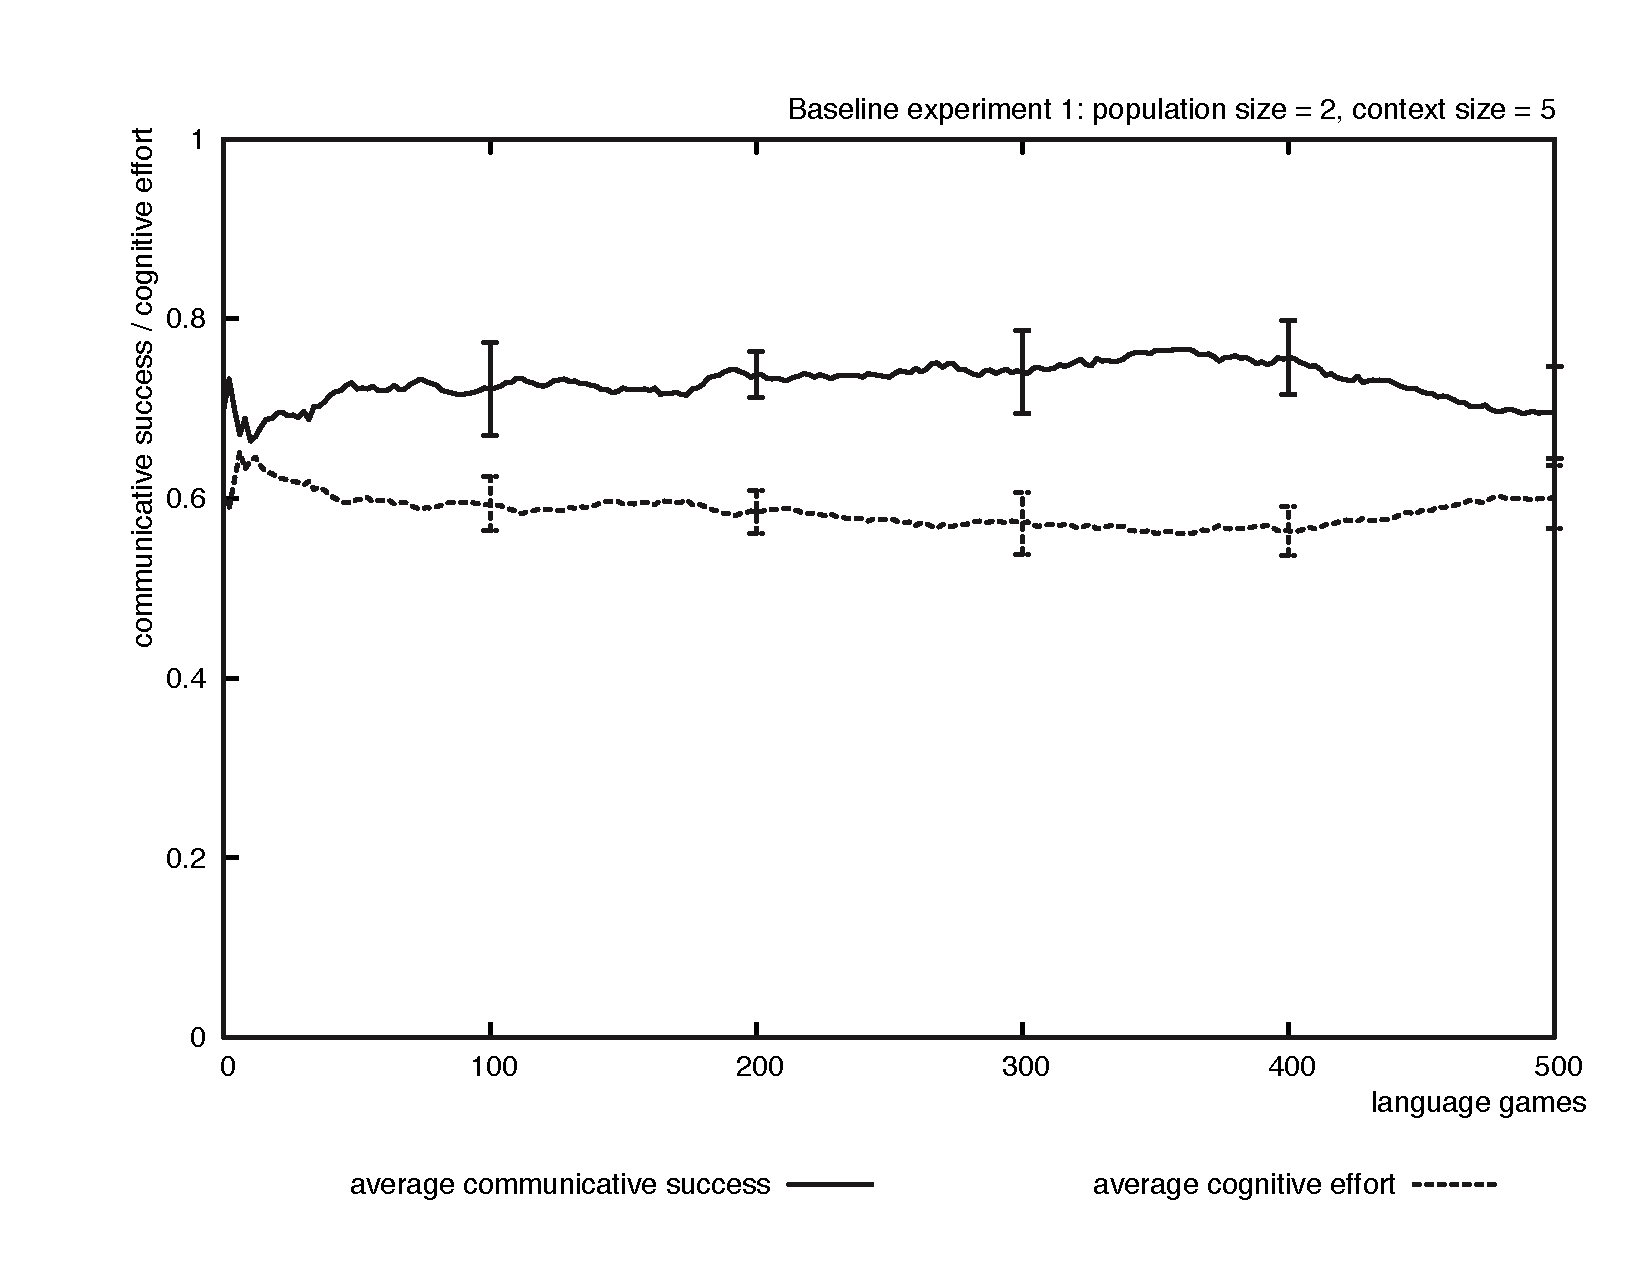
\includegraphics[width=\textwidth]{Chapter3/figs/graph-base1-effort2}}
  \caption[Baseline experiment 1: success and effort]{This graph shows the average cognitive effort\is{cognitive effort} and communicative success\is{communicative success} in baseline experiment 1 for 10 series of 500 language game\is{language game}s in a population\is{speech population} of two agents and a context size of five events. Success is reached in about 70\% of the games. Cognitive effort\is{cognitive effort} during interpretation amounts to 0,6 on average.}
   \label{f:base1-effort2}
\end{figure}


\subsubsection{Discussion}
 The results of baseline experiment 1 demonstrate that the agents can still reach communicative success\is{communicative success} if they use their world model for inferring the intended meaning. The proposed machinery thus works but only under certain conditions. For one thing, the hearer needs to have witnessed the scene in order to make the correct inferences. Second, the context cannot be too ambiguous otherwise interpretation can involve multiple hypotheses. As can be read from the average communicative success\is{communicative success} measure, this happens in 30\% of the cases. Failed games typically occur when the scene contains at least two event token\is{event token}s which have the same event type\is{event type} but which involve different participants.

Improving communicative success\is{communicative success} in the failed games could be achieved in many ways: agents can be given more complex dialogue\is{dialogue} strategies, the speaker can use pointing, the hearer can be more bold in making assumption\is{assumption}s about the speaker's intention or ask for additional feedback, etc. These strategies would however involve more negotiat\is{negotiation}ion and do not reduce the cognitive load during interpretation for the hearer. Additional marking, however, would be a solution which could resolve ambiguity\is{ambiguity} and reduce cognitive effort\is{cognitive effort} during interpretation at the same time. This solution will be tested in the next baseline experiment.

\section{Baseline experiment 2: specific marking}
\label{s:base2}

Baseline experiment 1 showed how agents can still reach communicative success\is{communicative success} without using grammar. In the second baseline experiment, agents can exploit this ability to autonomously detect whether it might be useful to make changes to their linguistic inventor\is{linguistic inventory}ies in order to optimize communication. The hypothesis investigated here can be formulated as follows: {\bfseries ambiguity\is{ambiguity} or too much cognitive effort\is{cognitive effort} during parsing and interpretation can be a trigger for the invention of functional marker\is{case!case marking}s for optimizing communicative success\is{communicative success}}.

\subsection{Speaker-based innovation}
\is{innovation}

\begin{figure}[t]
\centerline{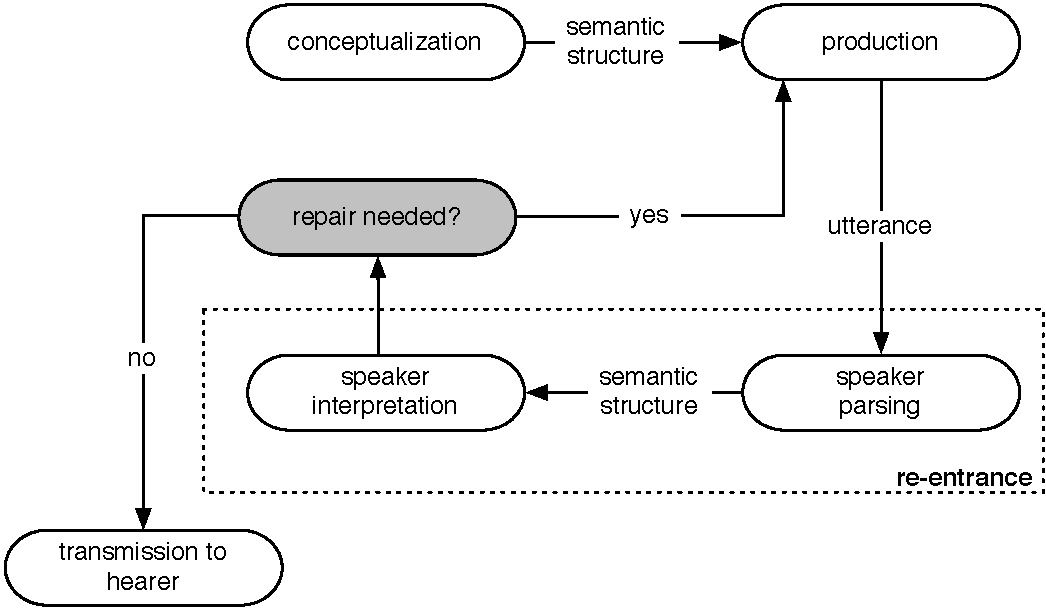
\includegraphics[width=\linewidth]{Chapter3/figs/re-entrance}}
  \caption[Speaker re-entrance]{Before transmitting an utterance to the hearer, the speaker `re-enters' her own utterance in her language system and uses herself as a model of the hearer. In this way the speaker estimates whether there might be problems or too much complexity for the hearer during parsing. If so, the speaker tries to repair\is{learning strategies!repair strategies} the problem.}
   \label{f:re-entrance}
\end{figure}

In baseline experiment 1 the hearer is faced with the cognitive load of figuring out who's doing what in events during each interaction. Moreover, if the context is complex enough it may not be clear which event the speaker was referring to. In this experiment, the agents are therefore endowed with a second key cognitive ability which involves the {\bfseries innovat\is{innovation}ion and expansion} of their language through event-specific marker\is{case!case marking}s. This ability comprises three subparts:

\begin{enumerate}
\item Expanding the agents architecture with a `re-entrant' mapping for detecting opportunities for optimization and learning innovat\is{innovation}ions;
\item Endowing the agents with the capacity of inventing a marker\is{case!case marking} and the corresponding constructions;
\item Endowing the agents with a consolidation\is{consolidation} mechanism which allows them to converge on a shared set of marker\is{case!case marking}s.  
\end{enumerate}

\subsubsection{Re-entrance}
\is{re-entrance}
 In baseline experiment 1, the agents could confidently use their lexical items to communicate with each other since the lexicon\is{lexicon} in this model is fixed, unambiguous, and shared by all the agents. However, should this scaffold\is{scaffold} be taken away, the agents would have to worry about whether the words they use are also known and understood by the other agents. They would thus somehow have to be capable of predicting the parsing and interpretation behaviour of the hearer in order to increase the chances of reaching communicative success\is{communicative success}. This can be achieved through `re-entrance\is{re-entrance}' 
\citep{steels03language} -- also called the `obverter' strategy by \citet{smith03intelligent}.

Re-entrance\is{re-entrance} can be thought of as self-monitoring\is{monitoring} in which the speaker does not directly transmit his utterance to the hearer, but first `re-enters' the utterance into his own linguistic system and parses and interprets the utterance himself as if he was the hearer. By taking himself as a model to simulate the linguistic behaviour of the hearer, the speaker can detect whether there might be problems or difficulties during parsing and interpretation. If so, the speaker will try to solve this problem. This strategy is illustrated in Figure \ref{f:re-entrance}. Similarly, the hearer can also use a re-entrant mapping for simulating the behaviour of the speaker. Technically speaking, achieving re-entrance\is{re-entrance} is not so difficult since the agents in these experiments can act both as a speaker and as a hearer.

Re-entrance\is{re-entrance} is thus a crucial strategy in inferential coding system\is{inferential coding system}s: if the speaker wants to solve a problem through innovat\is{innovation}ion, he needs to have an educated guess about the hearer's knowledge and which aspects of the common ground can be exploited for getting the message across. The hearer has to perform the same kind of reasoning for guessing the speaker's intentions. Human language users obviously adapt their linguistic behaviours to their speech partners (e.g. when speaking to children or second language learners). Given the fact that all agents in the experiments are each other's peers, the best model they can have of other agents is themselves.


\subsubsection{Innovation}
 It is unavoidable that language users come across situations in which the speaker does not know an adequate and well-entrench\is{entrenchment}ed convention\is{convention} for expressing a certain meaning, especially in the extreme case where there is no grammar at all. In this experiment, the speaker will invent a specific marker\is{case!case marking} for explicitly expressing a particular participant role\is{participant role} if there are possible ambiguities in the context or if the hearer needs to do more inference than is desirable. This is implemented through {\bfseries diagnostic\is{learning strategies!diagnostics}s and repair\is{learning strategies!repair strategies} strategies} which run in this experiment along the following algorithm:

\begin{enumerate}
\item {\bfseries Diagnostic 1:} Re-enter the utterance into the linguistic system and start a parsing and interpretation task.
\begin{enumerate}
\item[a.] If interpretation returns a failure or multiple hypotheses, report a problem;
\item[b.] If there is one possible hypothesis which contains at least one unexpressed variable equal\is{variable equality}ity, report a problem;
\item[c.] If there is no inference needed and if there is only one hypothesis, transmit the utterance to the hearer.
\end{enumerate}
\item {\bfseries Repair strategy 1:} If a problem of ambiguity\is{ambiguity} or unresolved variable equal\is{variable equality}ities has been reported, trigger repair\is{learning strategies!repair strategies} strategy 1.
\begin{enumerate}
\item[a.] If there is only one unexpressed variable equal\is{variable equality}ity, invent a new marker\is{case!case marking} for it and start a new production task;
\item[b.] If there are more than one unexpressed variable equal\is{variable equality}ities left (i.e. the repair\is{learning strategies!repair strategies} is too difficult), ignore the problem and transmit the utterance to the hearer.
\end{enumerate}
\end{enumerate}

I will now illustrate this algorithm with a concrete example. Suppose that the speaker and hearer both observe the same scene as the one used in section \ref{s:base1} in which Jack was walking to Jill; and that the sensory-motor processing delivers the same facts as in example \ref{facts}. This time the speaker only profiles the part of the event involving Jack and conceptualizes the following meaning:

\ea
\begin{lstlisting}
(jack object-1)
 (walk-to event-1 true)
 (walk-to-1 event-1 object-1)
 (walk-to-2 event-1 object-2)
\end{lstlisting}
\z

Since the speaker has no grammar yet, only the lexical entr\is{lexical entry}ies of {\em Jack} and {\em walk-to} are unified and merged with the coupled feature structure\is{feature structure!coupled feature structure} which results in the following, randomly ordered utterance:

\ea
``jack walk-to''
\z

Instead of directly transmitting the utterance to the hearer, the speaker first re-enters the utterance into her own linguistic system and parses the following meaning:

\ea
\begin{lstlisting}
(jack ?object-a)
 (walk-to ?event-1 true)
 (walk-to-1 ?event-x object-x)
 (walk-to-2 ?event-x object-y)
\end{lstlisting}
\z

Interpreting this meaning by unify\is{unify and merge}ing it with the speaker's world model yields the following set of bindings:

\ea
\begin{lstlisting}
((?event-x . event-1) (?object-x . object-1)
  (?object-y . object-2) (?object-a . object-1))
\end{lstlisting}
\z

Unification is successful and returns only one hypothesis so the speaker does not detect ambiguity\is{ambiguity}. However, there is a variable equal\is{variable equality}ity left between the variable `?object-x' and `?object-a': both refer to `object-1'. {\bfseries Diagnostic 1 will therefore report a problem that triggers repair\is{learning strategies!repair strategies} strategy 1}.

The repair\is{learning strategies!repair strategies} strategy assesses the difficulty of the problem: if there are more than one unexpressed variable equal\is{variable equality}ities left, the problem is classified as `too difficult to solve' and then the utterance is transmitted anyway. Here, however, there is only one variable equal\is{variable equality}ity so the speaker will invent a new marker\is{case!case marking} for it. This marker\is{case!case marking} is specific to the walk-to-1 role and can thus almost be seen as a lexical item itself. The speaker then invents a {\bfseries verb\is{verb}-specific construction\is{construction!verb-specific construction}} in which the new marker\is{case!case marking} (let's say {\em -bo}) binds the referent of the walk-to-1-role to the referent of the argument that fills this role by using the same variable `?object-x'. The syntactic pole states that this argument plays `syn-role-1' which is nothing more than a direct mapping of the walk-to-1-role.


\ea
\begin{lstlisting}
<Construction: construction-1
 ((?unit-1
   (meaning (== (walk-to ?event-x ?truth)
                (walk-to-1 ?event-x ?object-x)
                (walk-to-2 ?event-x ?object-y))))
  (?unit-2
   (referent ?object-x)))
<==>
 ((?unit-2
   (syn-role syn-role-1)))>
\end{lstlisting}
\z


The morphological rule states that the marker\is{case!case marking} immediately follows the argument which plays the walk-to-1-role. As explained in the previous Chapter, the morphological rule will create a new marker\is{case!case marking}-unit and make it a sub-unit of the argument-unit. Both the verb\is{verb}-specific construction\is{construction!verb-specific construction} and the morph-rule look slightly different from the original proposals by \citet{steels02simulating} due to changes in the grammar formalism, but they have the same performance\is{performance}.


\ea
\begin{lstlisting}
<Morph-rule: -bo
 ((?top-unit
   (syn-subunits (== ?unit-1)))
  (?unit-1
   (syn-role syn-role-1)))
<==>
 ((?top-unit
   (form (== (string ?marker-unit "-bo")
            (meets ?unit-1 ?marker-unit))))
  ((J ?marker-unit ?top-unit))
  ((J ?unit-1 ?top-unit (?marker-unit))))>
\end{lstlisting}
\z


The speaker now starts a new production task for the same meaning. In the initial node in the reaction network\is{reaction network}, the whole meaning is still grouped together in one unit. The speaker then unifies and merges the lexical entr\is{lexical entry}ies of {\em jack} and {\em walk-to} with the initial node which leads to a separate unit for each word. The new coupled feature structure\is{feature structure!coupled feature structure} looks as follows:


\ea
\begin{lstlisting}
<Node-2: coupled-feature-structure
 ((top-unit
   (sem-subunits (jack-unit walk-to-unit)))
  (jack-unit
   (meaning ((jack object-1)))
   (referent object-1))
  (walk-to-unit
   (referent event-1))
   (meaning ((walk-to event-1 true)
              (walk-to-1 event-1 object-1)
              (walk-to-2 event-1 object-2))))
<==>
 ((top-unit
   (syn-subunits (jack-unit walk-to-unit)))
  (jack-unit
   (form ((string jack-unit ''jack''))))
  (walk-to-unit
   (form ((string walk-to-unit "walk-to")))))>
\end{lstlisting}
\z


Before the repair\is{learning strategies!repair strategies}, this would be the final node in the reaction network\is{reaction network}. This time, however, the speaker has the newly made construction at her disposal. Since this is a production task, the semantic pole of the construction needs to unify\is{unify and merge} with the semantic pole of node-2. This is successful: the construction needs any unit containing the meaning of a walk-to-event and another unit of which the referent is the same one as the referent of the walk-to-1-role (`object-1'). The syntactic pole of the construction then simply merges the feature-value pair `(syn-role syn-role-1)' to the argument-unit. The construction thus license\is{license}s the following node in the reaction network\is{reaction network}:


\ea
\begin{lstlisting}
<Node-3: coupled-feature-structure
 ((top-unit
   (sem-subunits (jack-unit walk-to-unit)))
  (jack-unit
   (meaning ((jack object-1)))
   (referent object-1))
  (walk-to-unit
   (referent event-1))
   (meaning ((walk-to event-1 true)
              (walk-to-1 event-1 object-1)
              (walk-to-2 event-1 object-2))))
<==>
 ((top-unit
   (syn-subunits (jack-unit walk-to-unit)))
  (jack-unit
   (syn-role syn-role-1)
   (form ((string jack-unit ''jack''))))
  (walk-to-unit
   (form ((string walk-to-unit "walk-to")))))>
\end{lstlisting}
\z


Next, the speaker can unify\is{unify and merge} and merge the new morph-rule with node-3. The left-pole of the morph-rule (which is syntactic, see section \ref{s:morph-rule}) looks for any unit containing the feature-value pair `(syn-role syn-role-1)' which is indeed present in the syntactic pole of node-3. Next, the right-pole of the morph-rule is merged with the right-pole of node-3:


\ea
\begin{lstlisting}
<Node-4: coupled-feature-structure
 ((top-unit
   (sem-subunits (jack-unit walk-to-unit)))
  (jack-unit
   (meaning ((jack object-1)))
   (referent object-1))
  (walk-to-unit
   (referent event-1))
   (meaning ((walk-to event-1 true)
              (walk-to-1 event-1 object-1)
              (walk-to-2 event-1 object-2))))
<==>
 ((top-unit
   (syn-subunits (jack-unit walk-to-unit)))
  (jack-unit
   (syn-subunits (bo-unit))
   (syn-role syn-role-1)
   (form ((string jack-unit ''jack''))))
  (bo-unit
   (form ((string bo-unit ''-bo'') (meets jack-unit bo-unit))))
  (walk-to-unit
   (form ((string walk-to-unit "walk-to")))))>
\end{lstlisting}
\z


The speaker has no other items that can be unified and merged so node-4 is the final node in the reaction network\is{reaction network}. The speaker then renders the form-features of the syntactic pole into an utterance. The ordering between the words {\em jack} and {\em walk-to} are still random, but the coupled feature structure\is{feature structure!coupled feature structure} specifies that the marker\is{case!case marking} {\em -bo} immediately follows {\em jack}. This results in the following utterance:

\ea
``jack -bo walk-to''
\z

The speaker now re-enters this utterance again into his linguistic system to check whether the innovat\is{innovation}ion has the intended effect. I will not repeat the entire trace of parsing here since this is completely analog\is{analogy}ous to the example given in Chapter \ref{c:ar}. Parsing the utterance yields the following meaning:

\ea
\begin{lstlisting}
(jack ?object-x)
 (walk-to ?event-x true)
 (walk-to-1 ?event-x object-x)
 (walk-to-2 ?event-x object-y)
\end{lstlisting}
\z

Note that this time, the meaning-predicates `jack' and `walk-to-1' share the same variable `?object-x'. Interpretation then returns the following set of bindings:

\ea
{\footnotesize\tt{((?event-x . event-1) (?object-x . object-1) \\ \hspace{3,3mm}(?object-y . object-2))}}
\z

As can be seen in the set of bindings, there are no unexpressed variable equal\is{variable equality}ities left so no additional inferences are needed. The speaker is thus satisfied with the utterance and transmits it to the hearer.


\subsubsection{Learning}
 Learning a new marker\is{case!case marking} is very similar to inventing one and is achieved through the same cognitive mechanisms. The hearer first observes the utterance and then parses it. If there are unknown strings, such as the marker\is{case!case marking} {\em -bo} which was just invented by the speaker, the hearer will ignore it and try to parse as much as possible. Then the hearer tries to interpret the parsed meaning. If there are unexpressed variable equal\is{variable equality}ities left, the same diagnostic\is{learning strategies!diagnostics} as was used by the speaker will report a problem. The repair\is{learning strategies!repair strategies} strategy then tries to find out whether the utterance contains elements which could carry this particular meaning or function.

\begin{enumerate}
\item {\bfseries Hearer diagnostic\is{learning strategies!diagnostics} 1:} Parse the utterance and interpret its meaning.
\begin{enumerate}
\item[a.] If interpretation returns a failure or multiple hypotheses, report a problem;
\item[b.] If there is one possible hypothesis which contains at least one unexpressed variable equal\is{variable equality}ity, report a problem;
\item[c.] If there is no inference needed and there is only one hypothesis, signal agreement to the speaker.
\end{enumerate}
\item {\bfseries Hearer repair\is{learning strategies!repair strategies} strategy 1:} If a problem of ambiguity\is{ambiguity} or unresolved variable equal\is{variable equality}ities has been reported, trigger repair\is{learning strategies!repair strategies} strategy 1.
\begin{enumerate}
\item[a.] If there is only one unexpressed variable equal\is{variable equality}ity, check whether there was one unknown string in the utterance. If so, add a new verb\is{verb}-specific construction\is{construction!verb-specific construction} to the inventory which records the unknown string as a marker\is{case!case marking} for the variable equal\is{variable equality}ity. If not, ignore the problem and signal agreement or disagreement to the speaker depending on success of the game;
\item[b.] If there are more than one unexpressed variable equal\is{variable equality}ities left or if there were multiple unknown strings, ignore the problem. Transmit success to the hearer if inference is nevertheless possible. 
\item[c.] If interpretation fails or leads to multiple hypotheses, ignore the problem and signal disagreement.
\end{enumerate}
\end{enumerate}

\subsubsection{Consolidation}
\is{consolidation}
 In the original two-agent simulations variety never occurs since the agents only observe each other's inventions except for the extremely rare cases in which the learning task was too difficult and the learner later on invents a different solution for the same problem. So consolidation\is{consolidation} is fairly trivial and means just storing the newly created or learned items in the linguistic inventor\is{linguistic inventory}y.

However, as soon as we scale up the experiments to multi-agent population\is{speech population}s involving at least three agents, a pool of synchron\is{synchronic}ic variation\is{variation} naturally arises since the agents can independently come up with different innovat\is{innovation}ions for the same problems. The agents therefore need to have an alignment strateg\is{alignment strategy}y that enables them to deal with the variety and to converge on a shared set of preferred marker\is{case!case marking}s.

\begin{figure}[htp]
\centerline{\begin{tabular}{c}
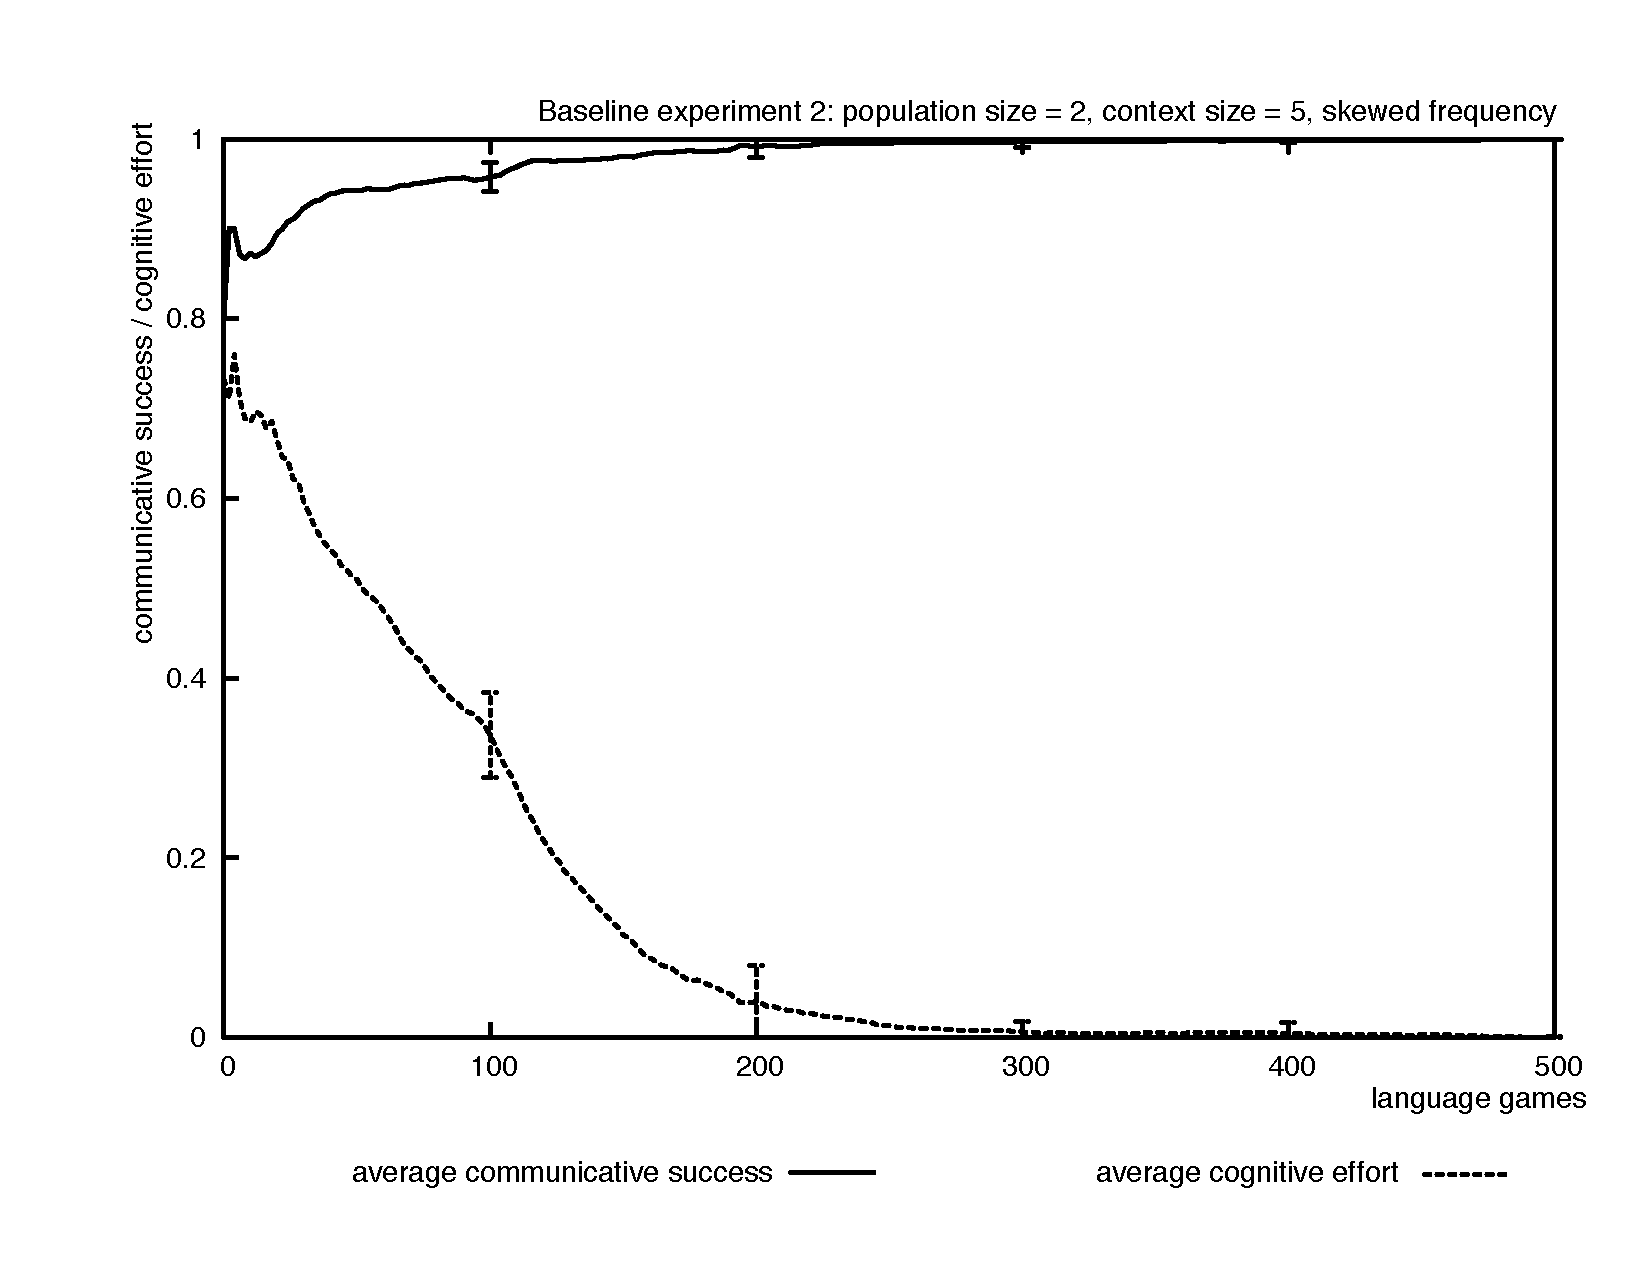
\includegraphics[width=0.8\linewidth]{Chapter3/figs/graph-base2-effort}
 \\
 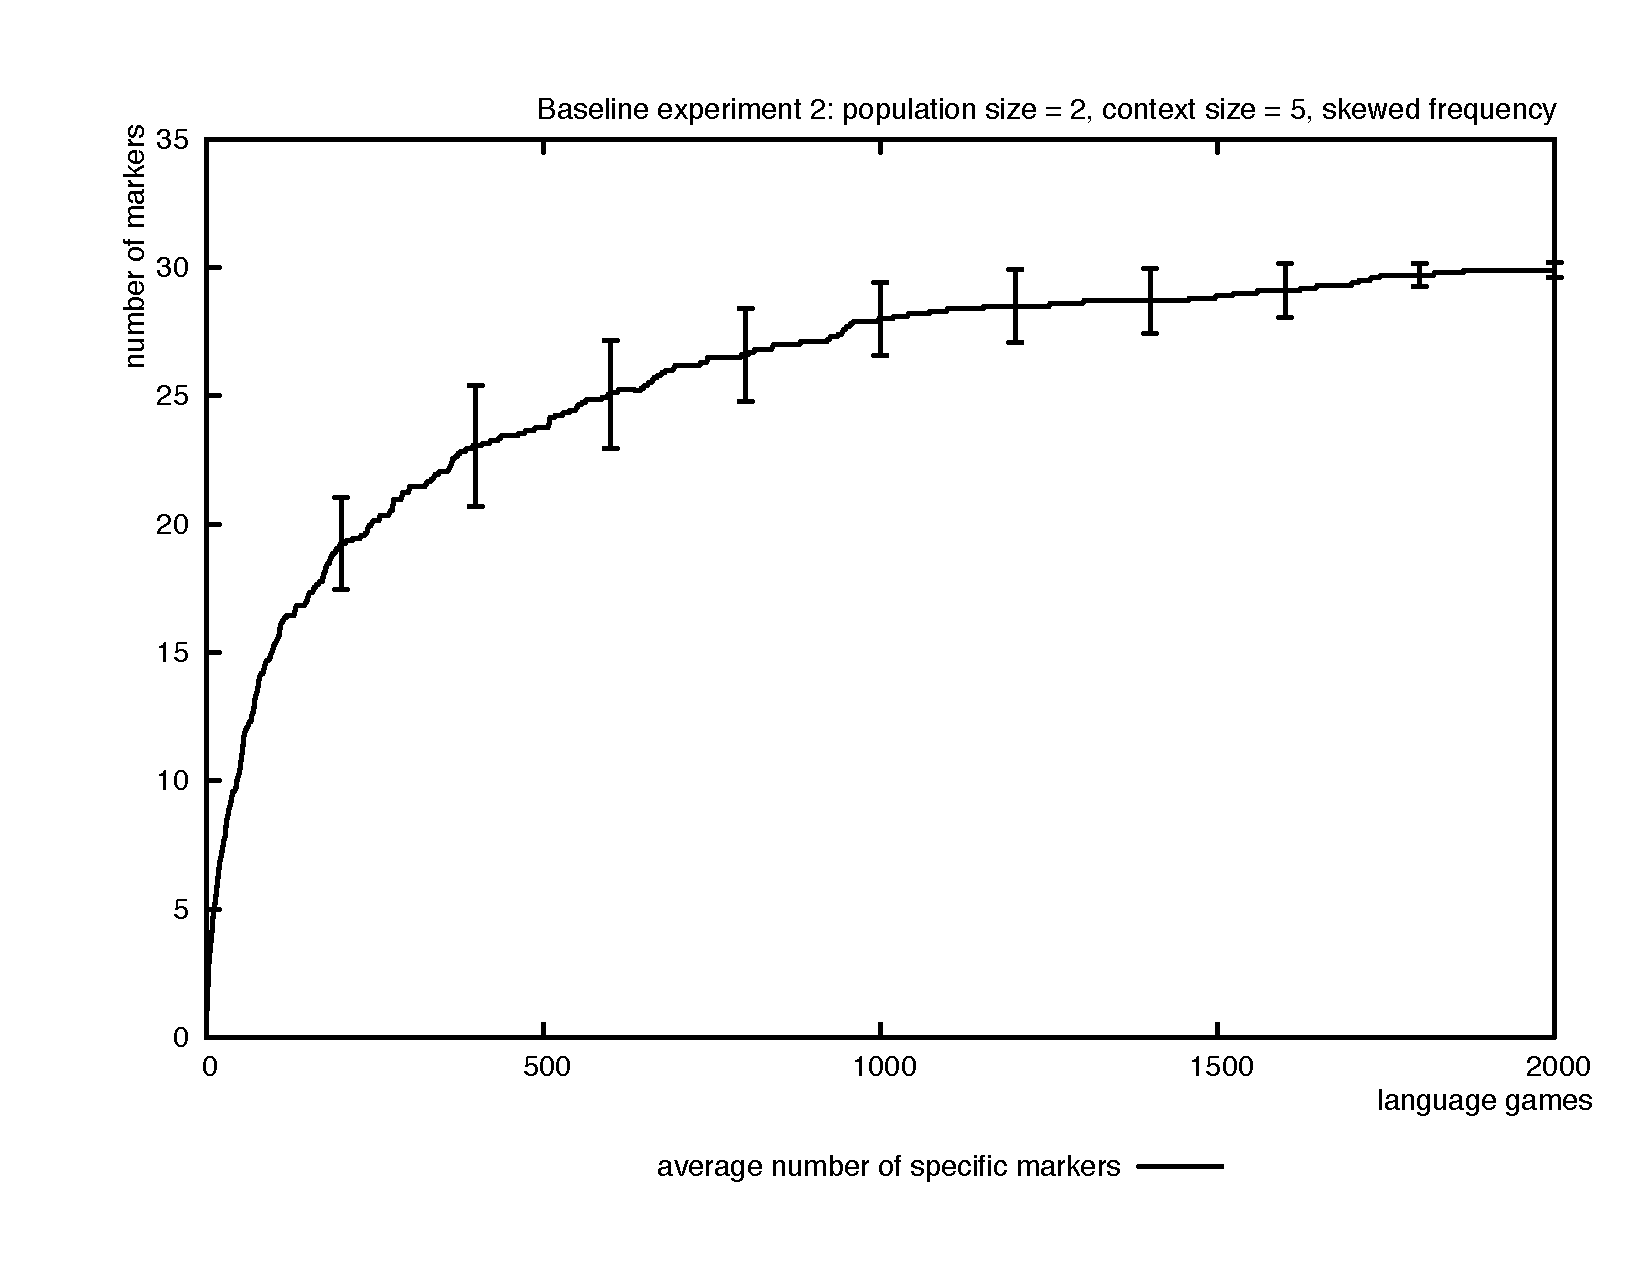
\includegraphics[width=0.8\linewidth]{Chapter3/figs/graph-base2-size}
  \end{tabular}}
  \caption[Baseline experiment 2: replication]{The top graph shows that the agents rapidly reach 100\% communicative success\is{communicative success} in the two-agent set-up. The agents also succeed in reducing the cognitive effort\is{cognitive effort} to zero. The bottom graph shows that they need to learn and store 30 specific marker\is{case!case marking}s in their inventory to do so.}
\label{f:base2-effort}
\end{figure}

In section \ref{s:towards-grammar} I argued that the experiments on grammar first of all try to move all the previous work on lexicon\is{lexicon} formation onto the domain of grammar, so this experiment starts with a similar alignment strateg\is{alignment strategy}y as was suggested in prior work. This strategy goes as follows: each construction has its own {\bfseries confidence\is{confidence} score} between 0 and 1. The higher the score, the more confident the agent is that the item is a convention\is{convention}alized unit in the population\is{speech population}. Based on the game's success and based on the speaker's behaviour, the hearer will update the scores in the inventory as follows:

\begin{itemize}
\item In case of success, increase the score of the applied construction(s) by 0.1 and decrease the scores of all its competit\is{competition}ors through {\bfseries lateral inhibition\is{lateral inhibition}} by 0.1. Competitors of a construction are constructions which either have the same semantic pole but a different form (competing synonyms), or the same form but different semantics (competing homonyms);
\item If the game was a failure, do nothing.
\end{itemize}

The fact that only the hearer performs score updating captures the intuition that agents first of all want to {\bfseries conform to} the behaviours of other agents in the population\is{speech population} rather than imposing their own preferences. A mathematical model by \citet{devylder07evolution} also shows that this strategy results in smoother convergence dynamics. In case of game failure, neither the speaker nor the hearer updates any scores. The reason for this is that the description game\is{language game!description game} does not offer enough explicit feedback for the agents to find out whether there might be parts in the processing chain which were harmful for communication.

\subsection{Results and discussion}

The above diagnostic\is{learning strategies!diagnostics}s and repair\is{learning strategies!repair strategies} strategies have been implemented and tested in three different simulations. The first series (set-up 2a) features a population\is{speech population} of two agents and replicates the results obtained by \citet{steels02simulating, steels04constructivist}. The second experiment (set-up 2b) involves a population\is{speech population} of ten agents in which the consolidation\is{consolidation} strategies become necessary for convergence. Both experiments feature the skewed frequency\is{frequency} of event type\is{event type}s mentioned in section \ref{s:world}. A third set-up (set-up 2c) also features 10 agents, but this time the skewed frequency\is{frequency} was replaced by an equal\is{variable equality} frequency\is{frequency} of event type\is{event type}s in order to study the convergence and competit\is{competition}ion dynamics more easily. All the results were obtained after ten series of language game\is{language game}s for each simulation.


\begin{figure}[phtb]
\centerline{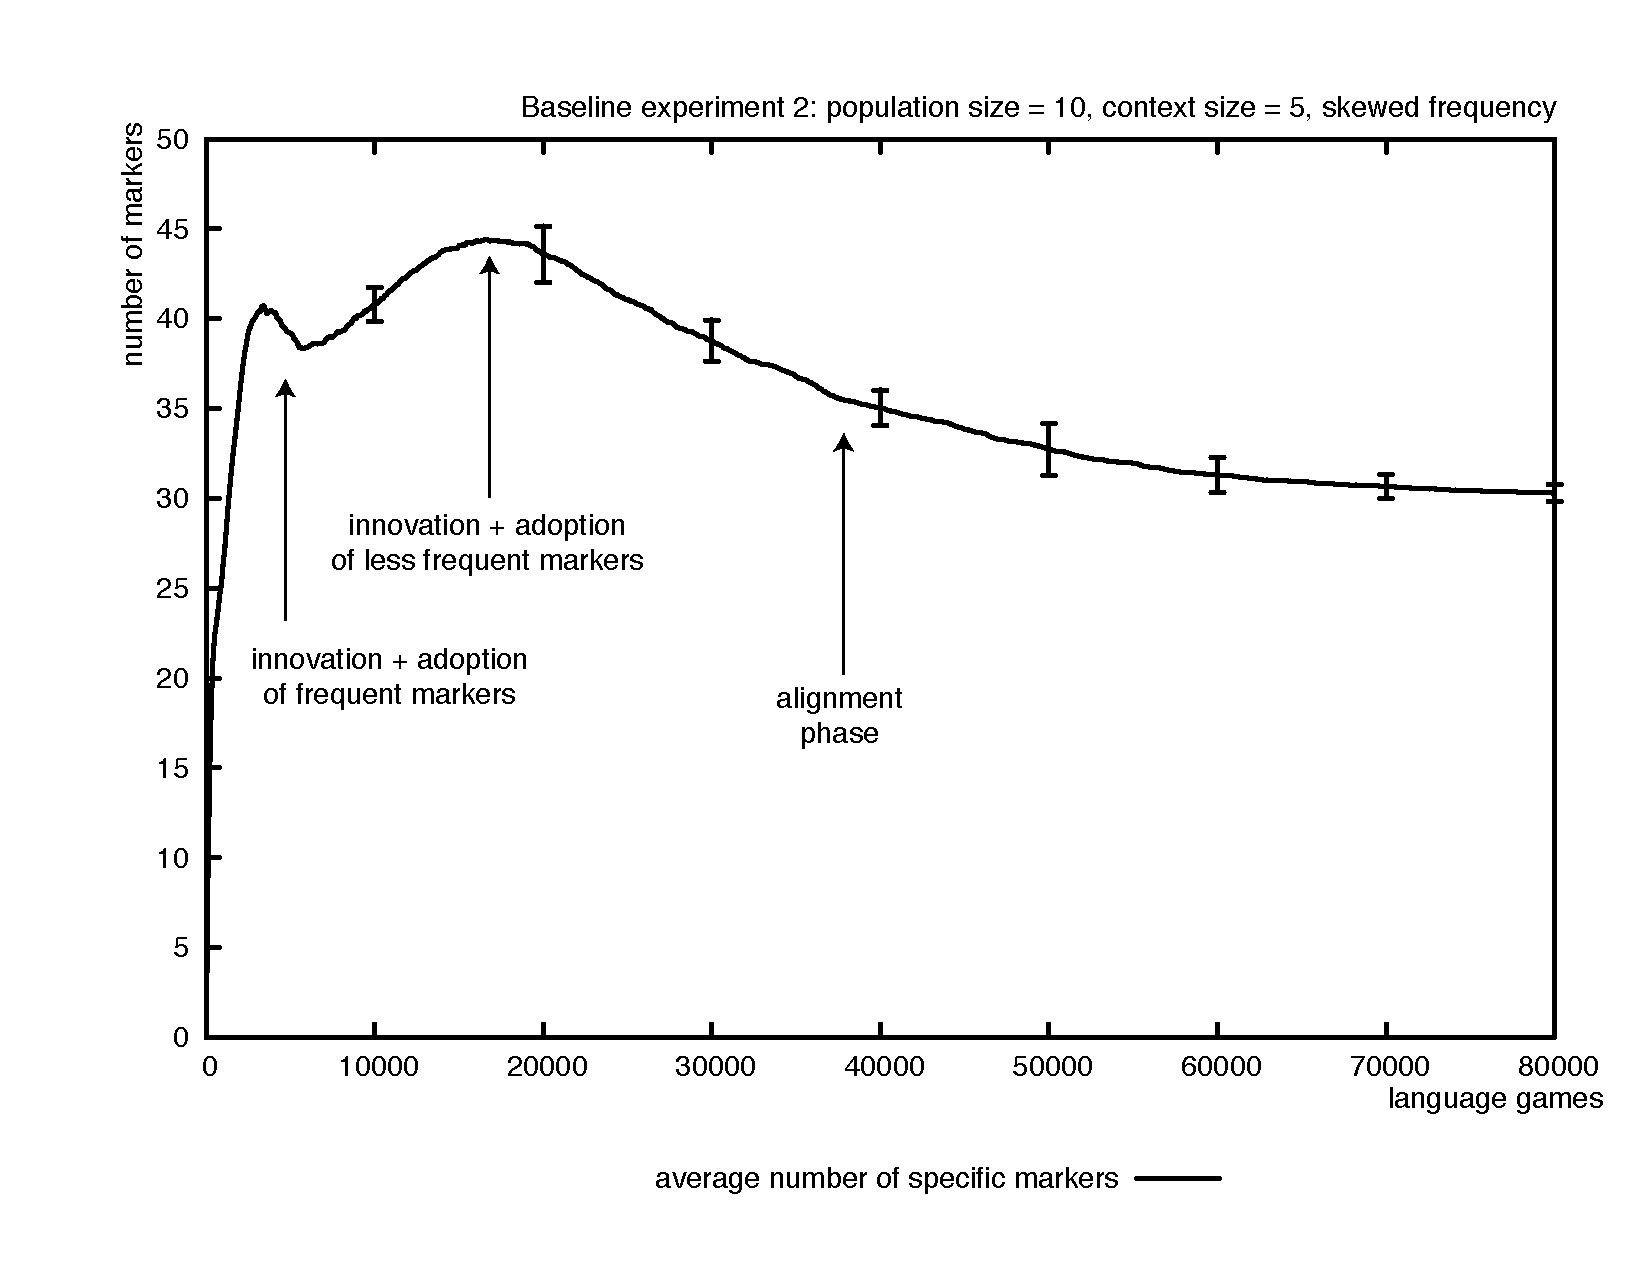
\includegraphics[width=\textwidth]{Chapter3/figs/graph-base2-size1}}
  \caption[Baseline experiment 2: number of markers (skewed frequency\is{frequency})]{This graph shows the number of specific marker\is{case!case marking}s in baseline experiment 2b for 10 series of 80.000 language game\is{language game}s in a population\is{speech population} of 10 agents and a context size of five events. The agents start innovat\is{innovation}ing and learning marker\is{case!case marking}s rapidly during the first 3.000 games after which a short period of alignment seems to kick in. The number of marker\is{case!case marking}s then rises again between game 7.000 and game 20.000. This is due to the skewed frequency\is{frequency} of the event-tyes: events that potentially take three participants are very rare in the data and marker\is{case!case marking}s for them are only now being acquired by all agents. Finally, a long alignment period starts which also takes much more time for the less-frequent event type\is{event type}s.}
   \label{f:base2-size1}
\end{figure}
\subsubsection{Results of set-up 2a}
 The results obtained from the replication experiment confirm the results of the original case experiment. The top graph in Figure \ref{f:base2-effort} shows that the average cognitive effort\is{cognitive effort} needed by the speaker rapidly drops to zero if the agents start inventing and using specific marker\is{case!case marking}s to indicate relations between events and their participants. With the marker\is{case!case marking}s the agents are also capable of overcoming ambiguity\is{ambiguity} in the context since communicative success\is{communicative success} rises to 100\%. However, there is a price to pay for this optimization, which is shown in the bottom graph: for each participant role\is{participant role}, the agents have to learn and store a specific marker\is{case!case marking} in the inventory. In this two-agent simulation, no variation\is{variation} occurs so agreeing on a set of 30 marker\is{case!case marking}s is fairly trivial.


\begin{figure}[ht]
\centerline{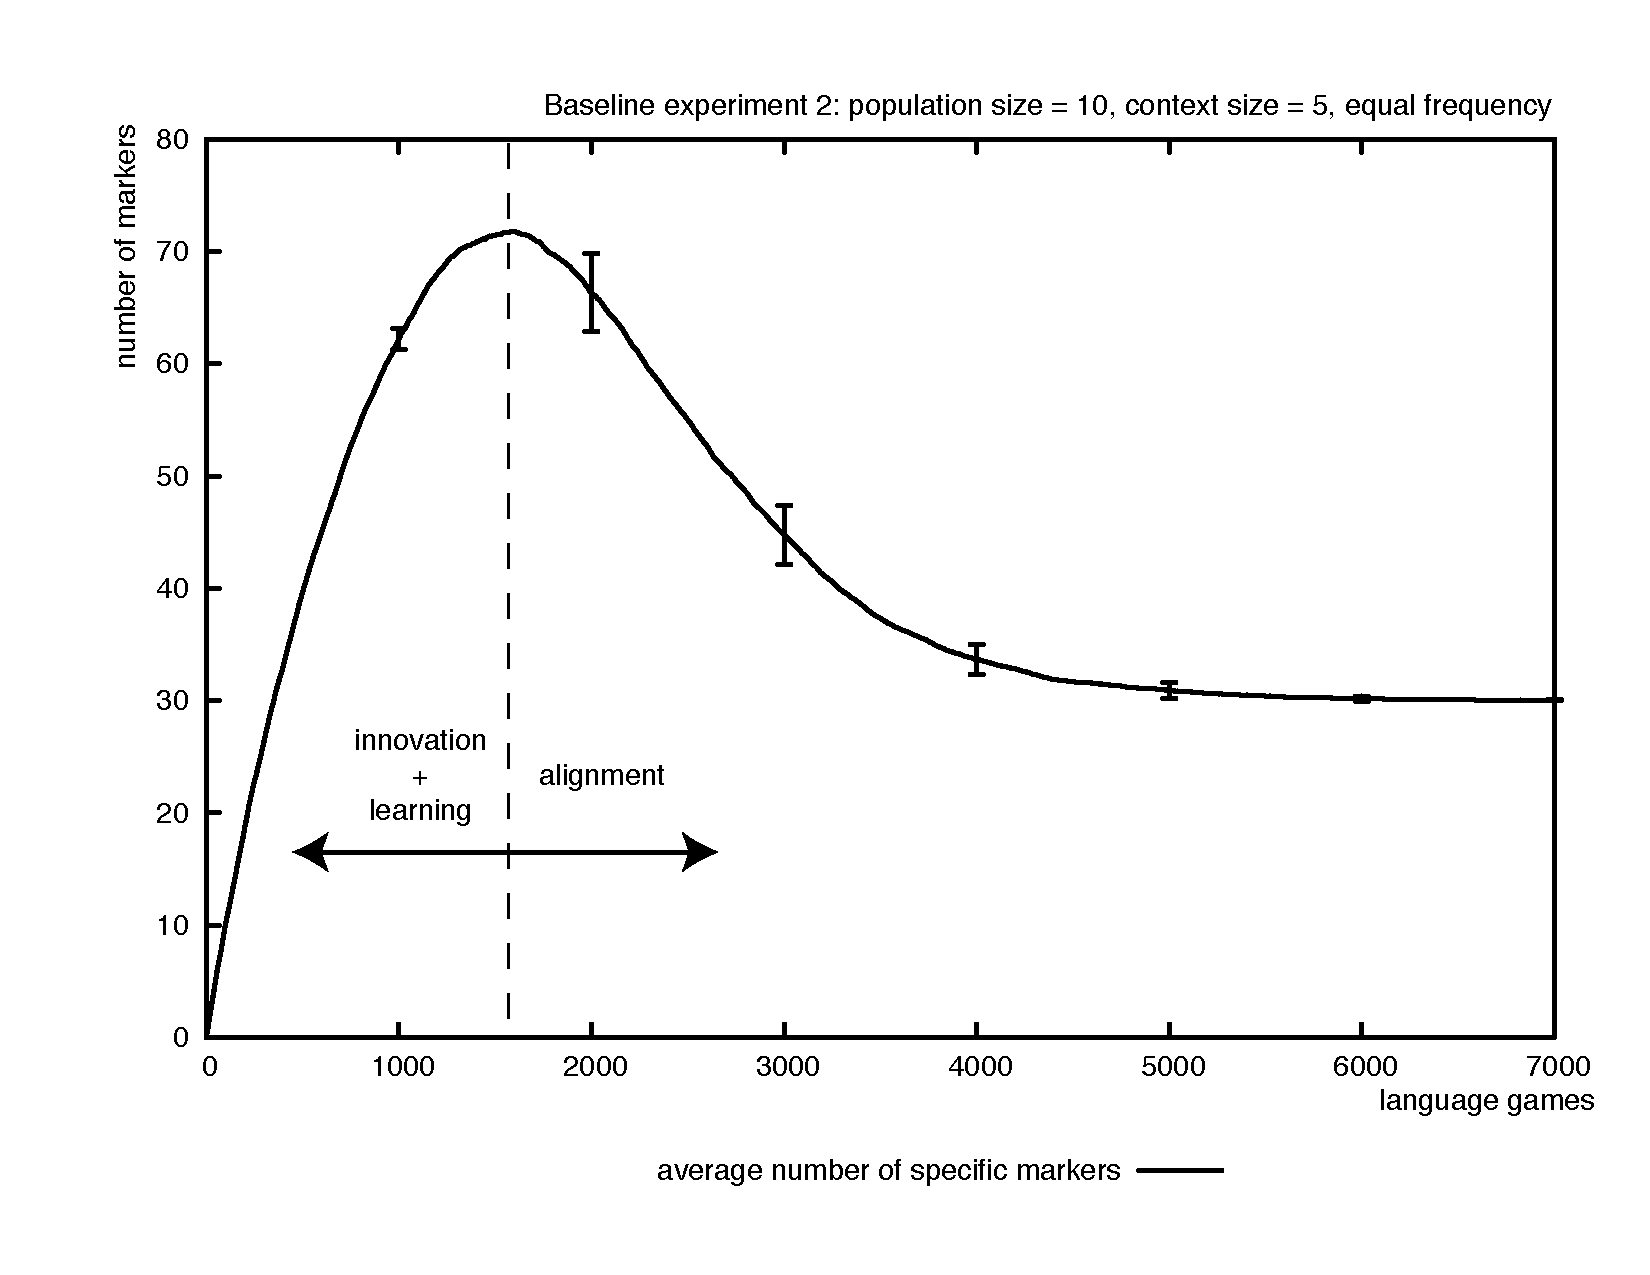
\includegraphics[width=0.8\textwidth]{Chapter3/figs/graph-base2-size2}}
  \caption[Baseline experiment 2c: number of markers (equal\is{variable equality} frequency\is{frequency})]{This graph shows the number of specific marker\is{case!case marking}s in baseline experiment 2c for 10 series of 7.000 language game\is{language game}s in a population\is{speech population} of 10 agents and a context size of five events. This case, all event type\is{event type}s occur with the same frequency\is{frequency} so we can see the convergence dynamics in the population\is{speech population} more clearly: agents invent and learn new marker\is{case!case marking}s during the first 1.500 language game\is{language game}s. The agents then need another 4.500 language game\is{language game}s in order to align their linguistic inventor\is{linguistic inventory}ies with each other.}
   \label{f:base2-size2}
\end{figure}
\subsubsection{Results of set-up 2b}
 If the population\is{speech population} size is increased, the agents need much more time to learn all the variation\is{variation}s floating in the population\is{speech population} and to converge on a shared set of 30 marker\is{case!case marking}s. As Figure \ref{f:base2-size1} shows, the agents need 80.000 language game\is{language game}s in order to agree on this set. This is still fairly rapid: it means that each agent needs to play an average of 8.000 games in order to conform to the language of its peers.

The graph first shows a steep rise to an average of 40 marker\is{case!case marking}s in the beginning after which an alignment phase seems to start. However, the number of marker\is{case!case marking}s starts to climb up again after 7.000 games and reaches a height of about 45 marker\is{case!case marking}s by the time 20.000 games have been played. Then there is a long and gradual slope towards convergence at 80.000 games. The two peaks in the graph are the result of the skewed frequency\is{frequency} of event type\is{event type} occurrences: marker\is{case!case marking}s for three-participant events are very rare and are therefore constructed, learned and propagat\is{propagation}ed later than the frequent marker\is{case!case marking}s. Even so, the agents still reach agreement and communicative success\is{communicative success} while reducing the cognitive effort\is{cognitive effort} needed if they are given enough time.


\begin{figure}[t]
\centerline{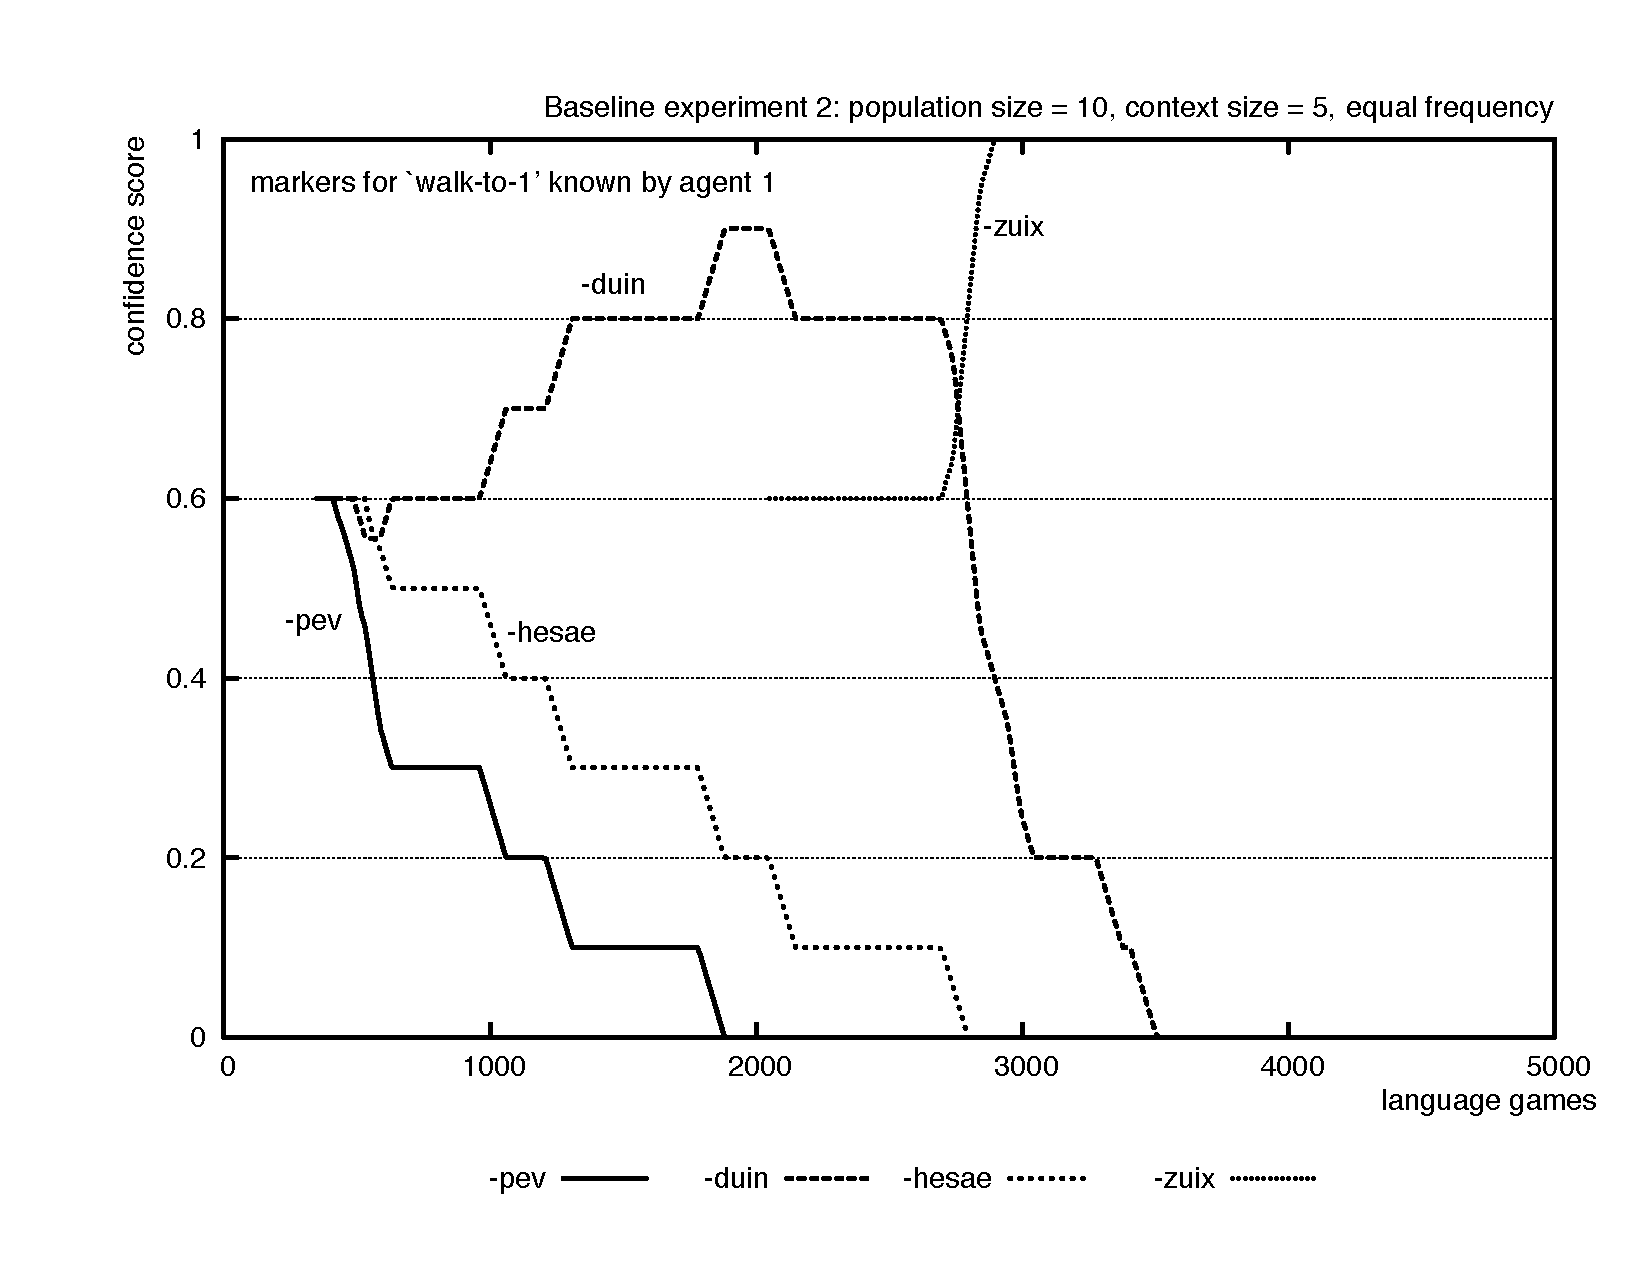
\includegraphics[width=0.87\textwidth]{Chapter3/figs/graph-base2-comp}}
  \caption[Baseline experiment 2: snapshot of competit\is{competition}ion (equal\is{variable equality} frequency\is{frequency})]{This graph shows a snapshot of the competit\is{competition}ion between forms for marking the participant role\is{participant role} `walk-to-1' within agent 1. Agent 1 learns the marker\is{case!case marking} {\em -pev} at first, but soon also observes {\em -duin} and {\em -hesae}. The marker\is{case!case marking} {\em -duin} seems to win the competit\is{competition}ion and even reaches a confidence\is{confidence} score of 0.9 after 2.000 language game\is{language game}s. However, the agent then learns another marker\is{case!case marking} {\em -zuix} which is apparently shared by a lot of other agents in the population\is{speech population}: at game 3.000 it has already pushed {\em -duin} down and it reaches 1.0 confidence\is{confidence} score.}
   \label{f:base2-comp}
\end{figure}
\subsubsection{Results of set-up 2c}
 In the third set-up all the event type\is{event type}s occur with the same frequency\is{frequency} so we can better study the convergence dynamics without other influences. Figure \ref{f:base2-size2} shows that the agents indeed need significantly less time than in the second set-up: between six and seven thousand language game\is{language game}s. On average this means about 600--700 games per agent, which comes close to the 500 games needed by the agents in two-agent simulations. The convergence task here is comparable in difficulty to a multiple word naming game\is{language game!multiword naming game} involving 30 objects \citep[see][]{vanlooveren05design}. The graph shows that the agents keep innovat\is{innovation}ing and learning new marker\is{case!case marking}s during the first 1.500 language game\is{language game}s after which they rapidly converge on a shared set of 30 marker\is{case!case marking}s. The peak of 70 marker\is{case!case marking}s -- as opposed to the peak of 45 with the skewed frequency\is{frequency} -- is normal since there are more competing marker\is{case!case marking}s floating in the population\is{speech population} at the same time.

Figure \ref{f:base2-comp} gives a snapshot of one agent's knowledge of marker\is{case!case marking}s for the participant role\is{participant role} `walk-to-1'. The agent learns three marker\is{case!case marking}s at about the same time: {\em -pev}, {\em -duin}, and {\em -hesae}. The marker\is{case!case marking} {\em -duin} seems to be the winning marker\is{case!case marking} and reaches a confidence\is{confidence} score of 0.9 by the time the agents have played 2.000 language game\is{language game}s. However, the agent then learns a new marker\is{case!case marking} {\em -zuix} which seems to be quite successful in the population\is{speech population}: its confidence\is{confidence} score rapidly increases to the maximum while {\em -duin} goes downhill very fast because of lateral inhibition\is{lateral inhibition}. In the end, {\em -zuix} wins the competit\is{competition}ion. 
\begin{figure}[t]
\centerline{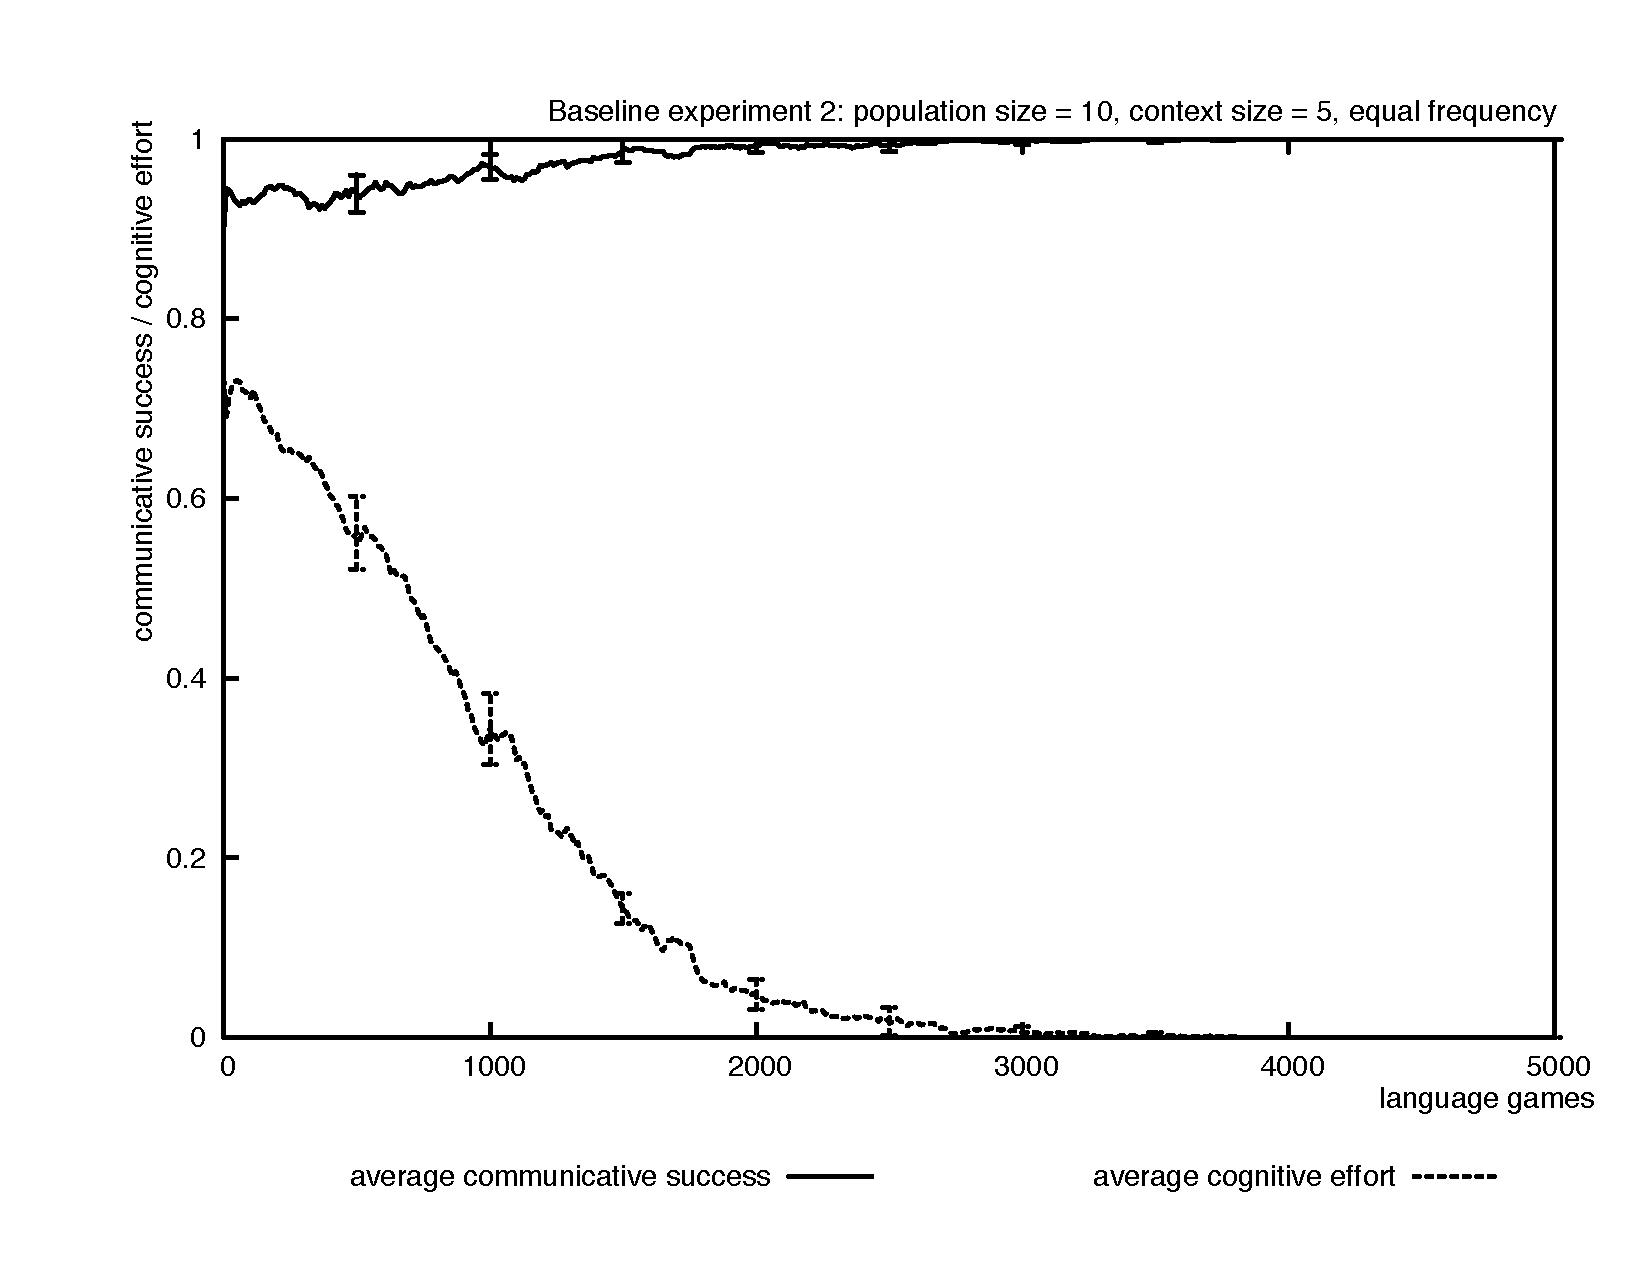
\includegraphics[width=\textwidth]{Chapter3/figs/graph-base2-effort2}}
  \caption[Baseline experiment 2: success and effort (equal\is{variable equality} frequency\is{frequency})]{In the multi-agent population\is{speech population}s too the agents succeed in reaching communicative success\is{communicative success} as well as reducing the cognitive effort\is{cognitive effort} needed for interpretation.}
   \label{f:base2-effort2}
\end{figure}

Finally, Figure \ref{f:base2-effort2} shows the average communicative success\is{communicative success} and cognitive effort\is{cognitive effort} again. The results show that the agents in the multi-agent simulations also rapidly reach 100\% communicative success\is{communicative success} by using marker\is{case!case marking}s. Cognitive effort\is{cognitive effort} also goes down until no inferences need to be made anymore.


\subsubsection{Discussion}
 The results of baseline experiment 2 clearly illustrate how agents can use locally available information\is{formation} to assess their own linguistic interactions and couple this assessment to repair\is{learning strategies!repair strategies} and consolidation\is{consolidation} strategies in order to improve communication. In this case, the agents mainly acted to reduce the semantic complexity of interpretation for the hearer: if additional marker\is{case!case marking}s are introduced for explicitly indicating the relations between events and their participants, parsing leads the agents immediately to the desired bindings in interpretation. Without the marker\is{case!case marking}s, additional inferences would still be needed.

However, a price has to be paid for reducing the effort of interpretation and that is an increased inventory size. During the language game\is{language game}s, the agents learn 70 marker\is{case!case marking}s on average and retain 30 of them, each one specific to a particular participant role\is{participant role}. The inventory size is in fact not the main problem here but a side-effect of a bigger issue: since the marker\is{case!case marking}s are restricted to one function only, the agents (given their present capabilities) cannot use them to go beyond the data of known events. Hence there is no generalization. Inventing new marker\is{case!case marking}s for each participant role\is{participant role} may be an efficient strategy in a small and fixed world, but becomes problematic once agents have to adapt to new meanings and communicative challenges.

Coupling these results back to natural languages, there are thus two clear qualitative differences: (a) marker\is{case!case marking}s in natural languages {\em do} generalize and become polysemous; and (b) they are not randomly invented but recruited from existing lexical items (see sections \ref{s:stage2} and \ref{s:stage3}). Both issues will have to be addressed in other experiments.


\section{Baseline experiment 3: semantic roles}
\is{semantic role}
\label{s:base3}

The results of baseline experiment 2 indicate that the agents can reduce the problem of ambiguity\is{ambiguity} and cognitive effort\is{cognitive effort} if they make use of additional marking. However, the proposed innovat\is{innovation}ion strategy requires new marker\is{case!case marking}s to be invented all the time so (a) there is no generalization beyond the known data, and (b) this may lead to an explosion of the inventory size in the long run. Baseline 3 investigates how the same principles of diagnosis and repair\is{learning strategies!repair strategies} in order to reach communicative success\is{communicative success} can lead to generalization. The hypothesis is that {\bfseries analog\is{analogy}ical reasoning over event structure\is{event structure}s can account for an increased generalization and productivity\is{productivity} of case marker\is{case!case marking}s}.

\subsection{Generalization as a side-effect}

When repair\is{learning strategies!repair strategies}ing a problem of unexpressed variable equal\is{variable equality}ties in the previous baseline experiment, the speaker assessed the repair\is{learning strategies!repair strategies} to be too difficult to learn if the context was too ambiguous. In a more complex simulation, however, one can imagine that ambiguity\is{ambiguity} is rather the rule than the exception so the speaker needs to innovat\is{innovation}e in a more clever way to give the hearer additional clues about what he meant. One such strategy is to reuse\is{reuse} existing items as much as possible in semantically related or analog\is{analogy}ous situations. In baseline experiment 3, the speaker can reuse\is{reuse} the existing marker\is{case!case marking}s in new situations by performing analog\is{analogy}ical reasoning over event structure\is{event structure}s. The analog\is{analogy}y algorithm comprises the following steps:

\begin{enumerate}
\item Given a target participant role\is{participant role}$_{i}$, find a source role$_{j}$ for which a case marker\is{case!case marking} already exists;
\item Elaborate the mapping between the two:
\begin{enumerate}
\item[a.] Take the target event structure\is{event structure} in which participant role\is{participant role}$_{i}$ occurs (provided by sensory-motor processing);
\item[b.] Take the source event structure\is{event structure} of the event that was used to create source role$_{j}$;
\item[c.] Select from the source event structure\is{event structure} all the facts and micro-events involving the filler of source role$_{j}$ and retrieve the corresponding facts and micro-events of the target event structure\is{event structure}. 
\end{enumerate}
\item Keep the mapping if it is good. A good mapping means that:
\begin{enumerate}
\item[a.] the filler of source role$_{j}$ always maps onto the same object in the corresponding facts and micro-events;
\item[b.] the corresponding object fills the target role$_{i}$ in in the target structure.
\end{enumerate}
\item If there are multiple analog\is{analogy}ies possible, choose the best one (based on entrench\is{entrenchment}ment and category size);
\item Build the necessary constructions and make the necessary changes to existing items.
\end{enumerate}

Step 3b in the algorithm ensures that an analog\is{analogy}ical role is also discriminating enough to distinguish the target role from other possible participant role\is{participant role}s in the same or other events. By reusing\is{reuse} existing items in novel but similar situations, the speaker reduces the hypothesis space for the hearer and facilitates the abduction\is{abduction} process. The hearer can retrieve the analog\is{analogy}y using the same algorithm if he also knows the other marker\is{case!case marking}. In this strategy, the generalization of existing linguistic items is not a goal in itself but rather a side-effect of optimizing communicative success\is{communicative success}.


\subsubsection{The target and the source}
 I will illustrate the analog\is{analogy}y algorithm of this experiment through an example. Suppose that the speaker wants to construct a marker\is{case!case marking} for the participant role\is{participant role} `walk-to-2' of the following walk-to-event:

\ea
\begin{lstlisting}
(walk-to event-100 true) (walk-to-1 event-100 jack)
   (walk-to-2 event-100 jill)
\end{lstlisting}
\z

I will from now on refer to `walk-to-2' as the {\em target role} and to `jill' as the {\em target filler}. Instead of inventing a new marker\is{case!case marking} immediately, the speaker will first check whether he already knows a marker\is{case!case marking} which is analog\is{analogy}ous and hence could be reuse\is{reuse}d. Suppose that the speaker already knows the marker\is{case!case marking} {\em -mi} for the participant role\is{participant role} `move-inside-1'. I will from now on refer to this participant role\is{participant role} as the {\em source role} and its filler as the {\em source filler}. The speaker has stored the original event which he used for creating the marker\is{case!case marking} and retrieves it from his memory:

\ea
\begin{lstlisting}
 
(move-inside event-163190 true) 
(move-inside-1 event-163190 jill)
(move-inside-2 event-163190 house-1)
\end{lstlisting}
\z

\subsubsection{Elaborate the mapping between the two}
 In order to elaborate the mapping between the two events, the complete event structure\is{event structure} is taken. The target event (walk-to) consists of four micro-events: one participant is moving and approaching another participant, which stands still until the two participants touch each other:

\begin{itemize}
 \item
\begin{lstlisting}
(move event-165641 true) (move-1 event-165641 jack)
\end{lstlisting}
\item
\begin{lstlisting}
(move event-165419 false) (move-1 event-165419 jill)
\end{lstlisting}
\item
\begin{lstlisting}
(approach event-165486 true) (approach-1 event-165486 jack)
(approach-2 event-165486 jill)
\end{lstlisting}
\item
\begin{lstlisting}
(touch event-165633 true) (touch-1 event-165633 jill)
(touch-2 event-165633 jack) 
\end{lstlisting}
\end{itemize}

 

The source event (move-inside) is made up of eight micro-events. The event starts with two visible participants, of which one is standing still. The distance between both objects becomes smaller as one participant moves to the other. This continues until they `touch' each other after which the moving participant disappears out of sight.

\begin{itemize}
\item \begin{lstlisting}
(visible event-161997 true) (visible-1 event-161997 jill)
\end{lstlisting}

\item \begin{lstlisting}
(visible event-161791 true) (visible-1 event-161791 house-1)
\end{lstlisting}

\item 
\begin{lstlisting}
(move event-161794 false) (move-1 event-161794 house-1)
\end{lstlisting}


\item\begin{lstlisting}
(distance-decreasing event-162441 true)
(distance-decreasing-1 event-162441 jill)
(distance-decreasing-2 event-162441 house-1)
\end{lstlisting}

\item 
\begin{lstlisting}
(touch event-161801 false) (touch-1 event-161801 jill)
  (touch-2 event-161801 house-1)
\end{lstlisting}

\item \begin{lstlisting}
(touch event-162493 true) (touch-1 event-162493 jill)
  (touch-2 event-162493 house-1)
\end{lstlisting}

\item\begin{lstlisting}
(borderscreen event-162377 false) (object-1 event-162377 jill)
\end{lstlisting}

\item \begin{lstlisting}
(visible event-162665 false) (visible-1 event-161997 jill)
\end{lstlisting}
\end{itemize} 

Analog\is{analogy}y is commonly defined as a mapping from a source domain to a new target domain. The next step in the algorithm is therefore to check how the existing role maps onto the target event structure\is{event structure}. This can be achieved by selecting all the micro-events of the source event that involve the source filler and map them onto the corresponding micro-events of the target. If the micro-events do not exist in the target event, they are ignored. Other information such as time-stamps and hierarchical structure is also ignored. This yields mapping in \figref{fig:3:mapping}.

\begin{figure}[h]
\footnotesize
 \begin{tabular}{lll} 
{\bfseries source event} & {\bfseries ==>} & {\bfseries target event} \\
\midrule
(touch-1 event-162493 jill) &  ==> & (touch-1 event-165633 jill)\\
(touch-1 event-161801 jill) & ==> &  (touch-1 event-165633 jill)\\
\end{tabular} 
\caption{Please provide a caption}
\label{fig:3:mapping}
\end{figure}

\subsubsection{A good mapping}
 There are two requirements for a mapping to be good. The first is that the source filler must always map onto the same object in the target structure. This is indeed the case in the above example: `jill' always maps onto `jill' in the target event. The algorithm thus found an analog\is{analogy}y between the source role and a role in the target event. The second requirement for a good mapping is that this corresponding role is the same one as the target role. Again, this is the case in the example: `jill' was indeed the target filler of the target role `walk-to-2'. The speaker can thus decide that the existing marker\is{case!case marking} {\em -ma} can be reuse\is{reuse}d.

In this example, the speaker does not have any other marker\is{case!case marking}s yet to check for analog\is{analogy}y. If there would be competing analog\is{analogy}ies, {\bfseries type frequency\is{type frequency}\is{frequency}} decides which analog\is{analogy}y will be chosen (i.e. the semantic role\is{semantic role} which covers the most participant role\is{participant role}s, ranging from one to many). I follow the same definition of type frequency\is{type frequency}\is{frequency} as \citet[77]{bybee00three}:

\begin{quote}
[T]ype frequency\is{type frequency}\is{frequency} determines productivity\is{productivity}: type frequency\is{type frequency}\is{frequency} refers to the number of distinct lexical items that can be substituted in a given slot in a construction, whether it is a word-level construction for inflection\is{inflection} or syntactic construction specifying the relation among words. The more lexical items that are heard in a certain position in a construction, the less likely it is that the construction will be associated with a particular lexical item and the more likely it is that a general category will be formed over the items that occur in that position. The more items the category must cover, the more general will be its critical features and the more likely it will be to exten\is{extension}d to new items. Furthermore, high type frequency\is{type frequency}\is{frequency} ensures that a construction will be used frequently, which will strengthen its representational schema, making it more accessible for further use, possibly with new items.

As type frequency\is{type frequency}\is{frequency} can range from one to a very large number, so there are varying degrees of productivity\is{productivity} associated with ranges of type frequency\is{type frequency}\is{frequency}. 
\end{quote}

\subsubsection{Adapting the inventory}
 If no analog\is{analogy}y can be found, the agent will invent a new marker\is{case!case marking} as in baseline experiment 2. In this example, however, the agent already knows a suitable marker\is{case!case marking} and it will have to incorporate this new use in its inventory. There are basically two options: either a new verb\is{verb}-specific construction\is{construction!verb-specific construction} is created for `walk-to-2' featuring the same case marker\is{case!case marking} as the construction for `move-inside-1'; or the use of the existing construction is exten\is{extension}ded. In this experiment, the latter solution is tested.

\begin{figure}[htp]
\centerline{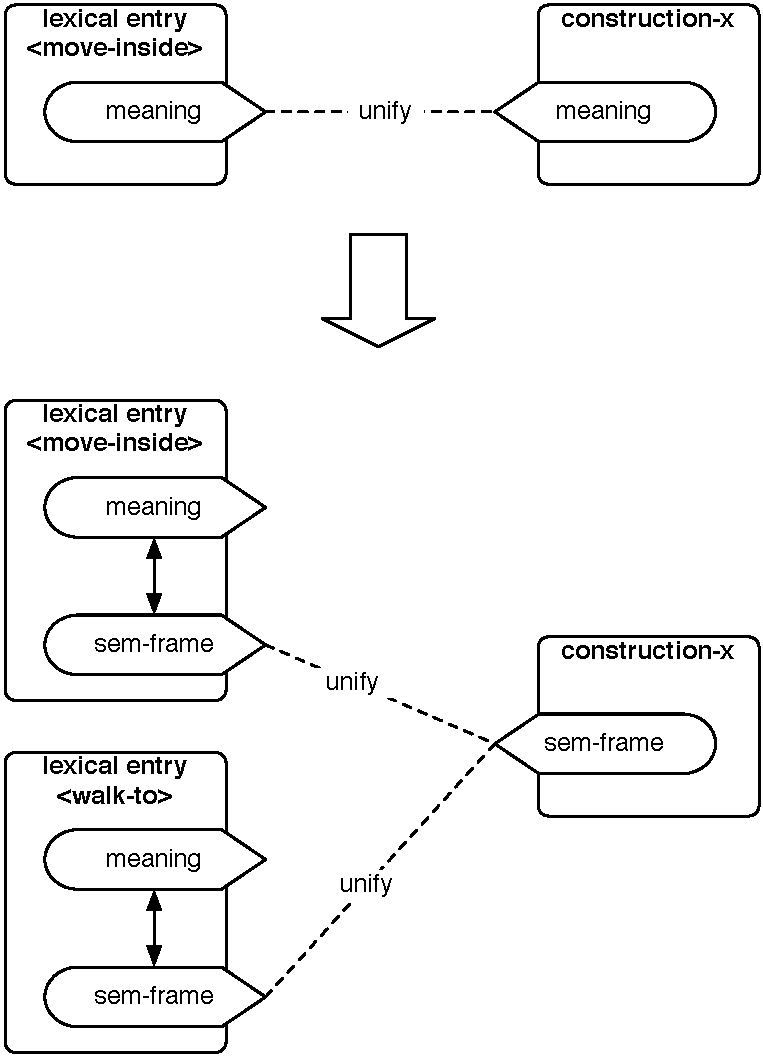
\includegraphics[width=0.7\linewidth]{Chapter3/figs/generalise}}
  \caption[Constructing generalized semantic role\is{semantic role}s]{This diagram shows how the semantics of lexical entr\is{lexical entry}ies and constructions integrate with each other. At first, constructions are verb\is{verb}-specific and unify\is{unify and merge} with the meaning of a lexical entr\is{lexical entry}y. If the agent however decides to reuse\is{reuse} this construction in a new situation, a generalized semantic role\is{semantic role} is constructed. The relevant lexical entr\is{lexical entry}ies are exten\is{extension}ded with a potential semantic frame\is{frame!semantic frame} which unifies with the semantic frame\is{frame!semantic frame} of the construction. The links between the meaning and the semantic frame\is{frame!semantic frame}s are taken care of by variable equal\is{variable equality}ities.}
   \label{f:generalise}
\end{figure}

The changes to the inventory are schematized in Figure \ref{f:generalise} and can be summarized as follows: the specific meaning in the semantic pole of the construction is removed and replaced by a semantic frame\is{frame!semantic frame} which contains the generalized semantic role\is{semantic role}. This semantic role\is{semantic role} shares the same variable as the referent of the other argument unit which was already present in the construction. The two lexical entr\is{lexical entry}ies which have to be compatible with the new construction ({\em move-inside} and {\em walk-to}) are exten\is{extension}ded with a semantic frame\is{frame!semantic frame} as well. As explained in Chapter \ref{c:ar}, this is not a frame in the traditional sense but rather a list of the potential valent\is{valency!potential valents}s of the verb\is{verb}. Since that Chapter also gives a full trace of parsing and production, I will not repeat the same operation here.


\subsubsection{Learning}
 The hearer learns the marker\is{case!case marking} by following the same strategy as before. If he didn't know the marker\is{case!case marking} yet, he will create a new verb\is{verb}-specific construction\is{construction!verb-specific construction} if the context is clear enough. If he already knew the marker\is{case!case marking}, he will get into trouble during parsing because its present use does not correspond to its previous function. The hearer will ignore the problem for the time being and parse the utterance as good as possible. Using the parsed meaning, inferred variable equal\is{variable equality}ities and re-entrance\is{re-entrance}, the agent can then (possibly) retrieve the analog\is{analogy}y introduced by the speaker. If the hearer cannot retrieve any analog\is{analogy}y, he will nevertheless accept it as imposed by the speaker.

The agents in this experiment can thus be characterized as (incremental) instan-ce-based\is{exemplar-based models} learners (and innovat\is{innovation}ors) \citep[Chapter 8]{mitchell97machine}: the agents are `lazy' learner\is{lazy learner}s in the sense that they postpone generalization until new instances have to be classified as opposed to `eager' learner\is{eager learner}s that try to make abstraction\is{abstraction}s over the data immediately. Each innovat\is{innovation}ion or novel classification is not based on abstract rules but by examining its relation to previously stored instances.  This kind of learning (and innovat\is{innovation}ion) fits usage-based model\is{usage-based model}s of language which presuppose {\em ``a bottom-up, maximalist, redundant approach in which patterns (schemas, generalizations) and instantiations are supposed to coexist, and the former are acquired from the latter''} \citep[20]{daelemans05memory}.


\subsubsection{Consolidation}
\is{consolidation}
 The original two-agent simulations did not need to care about alignment strateg\is{alignment strategy}ies or consolidation\is{consolidation} too much since the two agents always share the same communicative history. So the replicating experiment should pose no problems in both the alignment of case marker\is{case!case marking}s and the alignment of the internal structure of semantic role\is{semantic role}s. The same prediction cannot be made for multi-agent simulations in which alignment strateg\is{alignment strategy}ies are needed for convergence. Three additional set-ups have therefore been implemented: one which uses the same mechanism for updating the confidence\is{confidence} scores of linguistic items as in baseline experiment 2 (set-up 3b), one in which a more fine-grained scoring mechanism has been implemented (set-up 3c), and finally one in which (token) frequency\is{frequency} decides on the speaker's behaviour (set-up 3d). In this section I will not go into the reasons for experimenting with these different set-ups: they have been inspired by the experimental results and are therefore discussed later on. Instead, I will restrict myself to explaining the two new consolidation\is{consolidation} strategies. The four different set-ups (and their effects on the results) are summarized in Table \ref{t:consolidation-comparison}.


{\bfseries {\em Set-up 3c. }}The more fine-grained scoring mechanism implemented in set-up 3c is based on the idea that linguistic items are not `good or bad', but that they may be more suitable in some particular contexts and less suitable in others. A single confidence\is{confidence} score for every linguistic item cannot go beyond its black-or-white updating scheme and thus cannot handle a more nuanced way of processing. Instead, agents need more clever self-assess\is{self-assessment}ment criteria: next to communicative success\is{communicative success}, they can use {\bfseries co-occur\is{co-occurrence}rences} of linguistic items as a source for aligning their inventories. 

Co-occurring items are locally observable to the agents since they form one chain in the reaction network\is{reaction network} during processing. The general idea is reminiscient of Hebbian learning\is{Hebbian learning} (`what fires together, wires together'): a link is kept between co-occur\is{co-occurrence}ring items and a confidence\is{confidence} score is kept for this link based on the successful co-occur\is{co-occurrence}rence of both items. Suppose that the agent has the case marker\is{case!case marking} {\em -ma} (see the example earlier in this section) which may cover either the participant role\is{participant role} walk-to-2 or the role move-inside-1. The idea is now that the agents keep a link between co-occur\is{co-occurrence}ring linguistic items, so the agent would now have a link between construction-x one the one hand and the two lexical entr\is{lexical entry}ies {\em walk-to} and {\em move-inside} on the other. Instead of positing a score on the complete construction, each co-occur\is{co-occurrence}rence link has its own confidence\is{confidence} score: 

\ea
\parbox{\textwidth}{
  \begin{align*}
  \text{<Construction-x>} & \leftarrow  
  \begin{array}{ll} 
  0.5 \rightarrow & \text{<move-inside> (for move-inside-1) }\\
  0.5 \rightarrow & \text{<walk-to> (for walk-to-2)}
  \end{array}
  \end{align*}
}
\z

Suppose that the speaker also has the marker\is{case!case marking} {\em -bo} which can be used for marking `move-1' and `move-inside-2':

\ea
\parbox{\textwidth}{
  \begin{align*}
  \text{<Construction-y>} & \leftarrow  
  \begin{array}{ll} 
  0.5 \rightarrow & \text{<move-inside> (for move-inside-1)} \\
  0.5 \rightarrow & \text{<move> (for move-1)}
  \end{array}
  \end{align*}
  }
\z

If the agent then observes the co-occur\is{co-occurrence}rence of construction-x and {\em move-inside} (i.e. the agent analyzes an utterance in which {\em -ma} was used for marking move-inside-1), the score of the link is increased with 0.1 and the score of competing links (here the link between {\em move-inside} and construction-y) is decreased by 0.1. The other confidence\is{confidence} scores based on co-occur\is{co-occurrence}rence remain untouched:

\ea
\begin{align*}
\text{<Construction-x>} & \leftarrow  
\begin{array}{ll} 
0.6 \rightarrow & \text{<move-inside> (for move-inside-1) }\\
0.5 \rightarrow & \text{<walk-to> (for walk-to-2)}
\end{array}
\\
\text{<Construction-y>} & \leftarrow  
\begin{array}{ll} 
0.4 \rightarrow & \text{<move-inside> (for move-inside-1)} \\
0.5 \rightarrow & \text{<move> (for move-1)}
\end{array}
\end{align*}
\z

Note that this score is not the actual co-occur\is{co-occurrence}rence frequency\is{frequency}, but a confidence\is{confidence} score between 0 and 1 which only indirectly reflects co-occur\is{co-occurrence}rence and which is updated based on communicative success\is{communicative success}.


{\bfseries {\em Set-up 3d. }} The fourth set-up in baseline experiment 3 removes the explicit lateral inhibition\is{lateral inhibition} consolidation\is{consolidation} of the previous set-ups and replaces it with a combination of {\bfseries token frequency\is{token frequency}\is{frequency} and memory decay\is{memory decay}}. Frequency is implemented as a simple counter which can be updated after each interaction. This set-up has the following features:

\begin{itemize}
\item During production, the speaker will use the linguistic items which have the highest frequency\is{frequency} score;
\item After each {\em successful} interaction, the hearer will increase the counter of all the constructions that were applied during parsing by one;
\item When an agent has engaged in 50 interactions, all the frequency\is{frequency} scores are decreased by one (= memory decay\is{memory decay}).
\end{itemize}

This kind of (token) frequency\is{frequency} favours more general constructions: the larger the type frequency\is{type frequency}\is{frequency} of a certain class or category, the more chances it has to increase its token frequency\is{token frequency}\is{frequency}. The memory decay\is{memory decay} implemented here is unaffected by population\is{speech population} size since it is based on each agent's individual history. It is, however, sensitive to inventory size and frequency\is{frequency}: linguistic items can only survive if they occur at least once before the next decay is performed. In the present set-up, each participant role\is{participant role} occurs one time out of thirty interactions on average.

\subsection{Results and discussion of set-up 3a}

\begin{figure}[ht]
\centerline{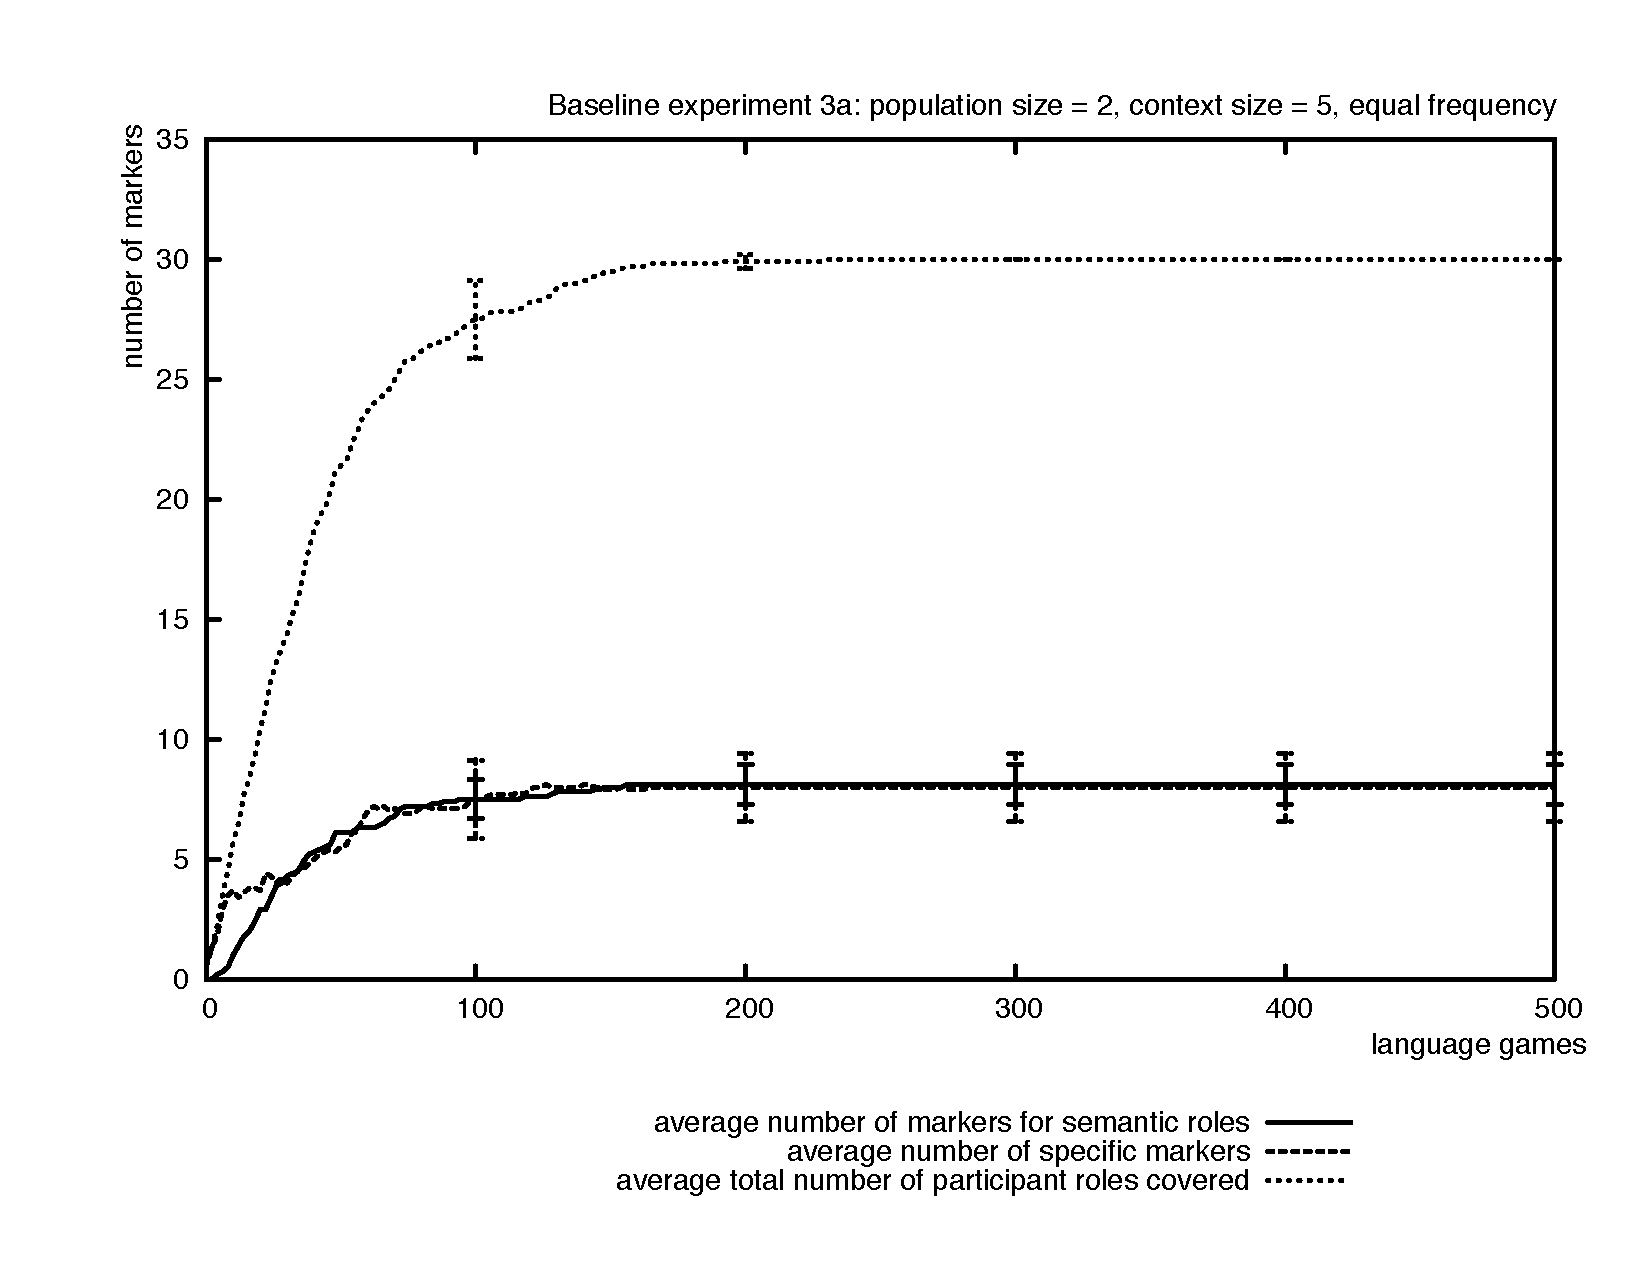
\includegraphics[width=0.9\textwidth]{Chapter3/figs/graph-base3-size3a}}
  \caption[Baseline experiment 3a: number of markers]{In the two-agent simulations, the agents have no problems aligning their inventories since there is no variation\is{variation} in the population\is{speech population}. In ten series of 500 language game\is{language game}s, the agents came up with an average of 6-8 marker\is{case!case marking}s for semantic role\is{semantic role}s and an average of 6-9 marker\is{case!case marking}s for specific participant role\is{participant role}s. The semantic role\is{semantic role}s gather together up to 24 participant role\is{participant role}s out of 30.}
   \label{f:base3-size3a}
\end{figure}

\subsubsection{Results}
 The replicating experiment featuring a population\is{speech population} of two agents confirms the results obtained by \citet{steels02simulating, steels04constructivist}. The agents succeed in reusing\is{reuse} existing marker\is{case!case marking}s and generalizing them to semantic role\is{semantic role}s as is shown in Figure \ref{f:base3-size3a} . During ten series of 500 language game\is{language game}s, the agents constructed on average 6 to 8 marker\is{case!case marking}s which could be used for covering at least two participant role\is{participant role}s. In total, up to 24 participant role\is{participant role}s out of 30 were grouped together in more general roles. In each simulation, also 6 to 9 marker\is{case!case marking}s survived which cover specific participant role\is{participant role}s.

A closer examination of the semantic role\is{semantic role}s learns us that they tend to be small generalizations mostly covering two participant role\is{participant role}s. Some roles exceptionally gather four or even six participant role\is{participant role}s. Here are some example sentences from one of the simulations and their glosses:

\ea
\gll jack -cui walk-to jill -ge \\
jack sem-role-6 walk-to  jill sem-role-26 \\
\glt `Jack walks to Jill.' \\

\item
\gll touch jill -cui house -shae \\
touch jill sem-role-6 house-1 sem-role-29 \\
\glt `Jill touches house-1.' \\

\item
\gll house -lu move-inside boy -cui \\
house-1 sem-role-10 move-inside boy sem-role-6 \\
\glt `The boy moves inside house-1.' \\

\z

In the same simulation, the following marker\is{case!case marking}s and their corresponding participant role\is{participant role}s were constructed (ranging from 7 specific marker\is{case!case marking}s to 8 more general ones):

\begin{itemize}
\item -vuh: cause-move-on-1
\item -yaem: cause-move-on-2
\item -jibui: cause-move-on-3
\item -shuip: give-3
\item -vot: take-3
\item -me: visible-1
\item -naez: move-outside-2
\item -zo: fall-1, approach-1
\item -tui: fall-2, approach-2
\item -shae: touch-2, give-2
\item -fe: distance-decreasing-1, grasp-1
\item -lu: move-inside-2, distance-decreasing-2
\item -we: move-1, give-1, take-1
\item -cui: walk-to-1, object-1, grasp-2, hide-2
\item -ge: touch-1, move-inside-1, move-outside-1, hide-1, walk-to-2, take-2
\end{itemize}

\subsubsection{Discussion}
 The results show that the construction of generalized semantic role\is{semantic role}s allows the agents to reduce the number of marker\is{case!case marking}s by 65--70\%. However, the most important observation is that by endowing the agents with the capacity of analog\is{analogy}ical reasoning, they are capable of generalization beyond previous linguistic experience as is shown in the increasing productivity\is{productivity} of some marker\is{case!case marking}s.

In the results there is still a fairly large residue of verb\is{verb}-specific marker\is{case!case marking}s which is partly due to the analog\is{analogy}y algorithm and partly due to the fact that only two agents were involved in the simulation. First, the analog\is{analogy}y algorithm is very strict in the sense that two roles are either analog\is{analogy}ous or not: there is no in-between value that allows for some flexibility. Second, since there are no variation\is{variation}s in the population\is{speech population}, the construction of semantic role\is{semantic role}s is entirely dependent on the linguistic history of both agents: once an analog\is{analogy}y is constructed and successfully applied in communication, the agents will not try to come up with better or more general analog\is{analogy}ies later on. In other words, the solutions that the two agents come up with may not be optimal given their search space so they end up in a local maximum. A larger population\is{speech population} may give this search an additional boost.

\subsection{Results and discussion of set-up 3b}

\begin{figure}[ht]
\centerline{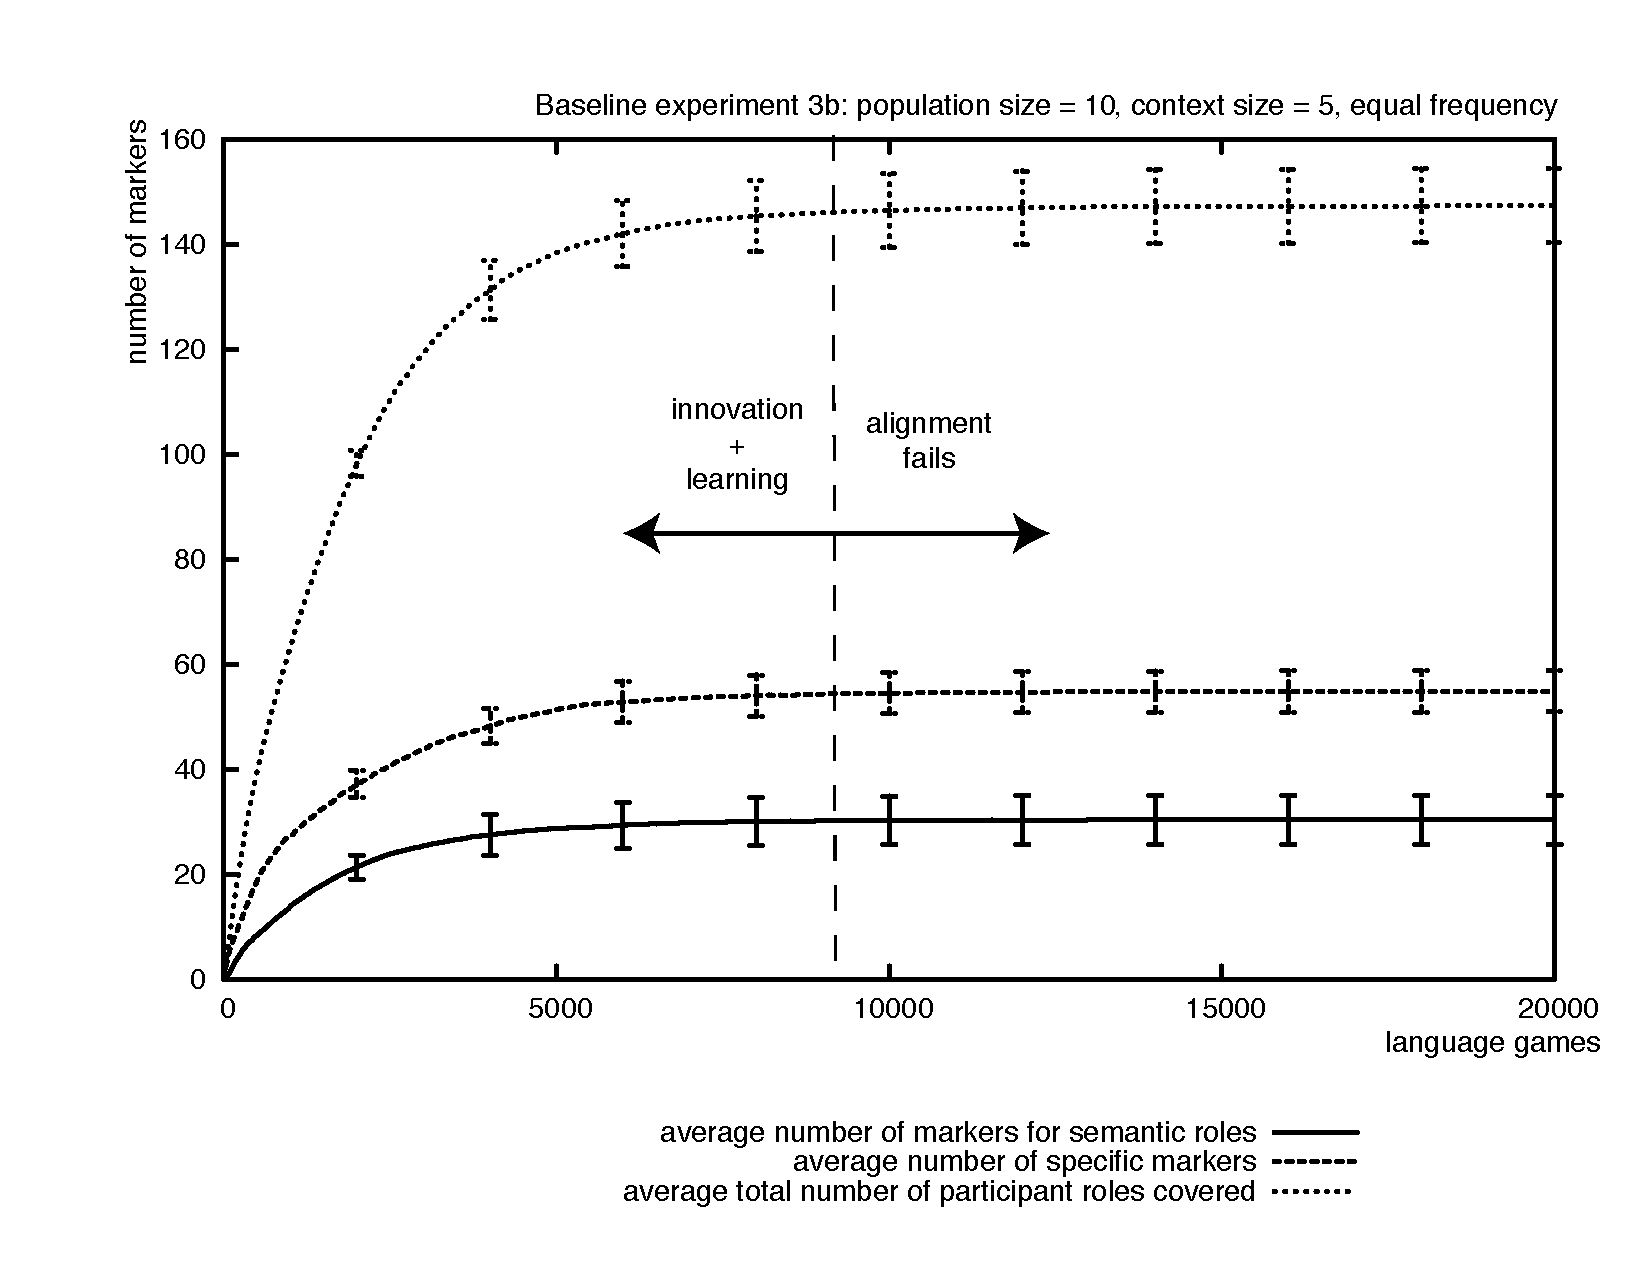
\includegraphics[width=0.9\textwidth]{Chapter3/figs/graph-base3-size3b}}
  \caption[Baseline experiment 3b: number of markers]{When scaling the experiments up to multi-agent simulations, the traditional alignment strateg\is{alignment strategy}ies used in prior experiments on lexicon\is{lexicon} formation\is{formation} are not sufficient for the population\is{speech population} to reach convergence. For thirty participant role\is{participant role}s, the agents have to remember 140 variation\is{variation}s to communicate successfully, which is an average of 4,7 possible ways for marking each participant role\is{participant role}.}
   \label{f:base3-size3b}
\end{figure}

\subsubsection{Results}
 In set-up 3b the population\is{speech population} size is increased to 10 agents so there will be more variation\is{variation} among the agents. This is indeed confirmed in Figure \ref{f:base3-size3b} which shows that there are a total of 140 variation\is{variation}s floating in the population\is{speech population} for marking 30 participant role\is{participant role}s. This is an average of 4,7 possible ways for marking each participant role\is{participant role}. This number of possibilities does not drop to 30, which is a first indication that the agents do not converge on a shared set of grammatical marker\is{case!case marking}s. As for the nature of the marker\is{case!case marking}s, the results indicate that there are about 20 marker\is{case!case marking}s that can be used for covering at least two participant role\is{participant role}s whereas there are about 50 specific participant role\is{participant role} marker\is{case!case marking}s as well. The average inventory size of the agents is thus far from optimal.

Figure \ref{f:base3-effort3b} confirms that the agents do not reach convergence: the meaning-form coherence indicates the degree to which the agents prefer the same case marker\is{case!case marking} for a particular participant role\is{participant role}. As the graph shows, coherence only reaches 40\% which means that the agents use a different marker\is{case!case marking} for the same participant role\is{participant role} in more than half of the language game\is{language game}s. Yet, as the graph also shows, the agents are capable of reaching 100\% communicative success\is{communicative success}  and reducing the cognitive effort\is{cognitive effort} to zero.
\begin{figure}[t]
\centerline{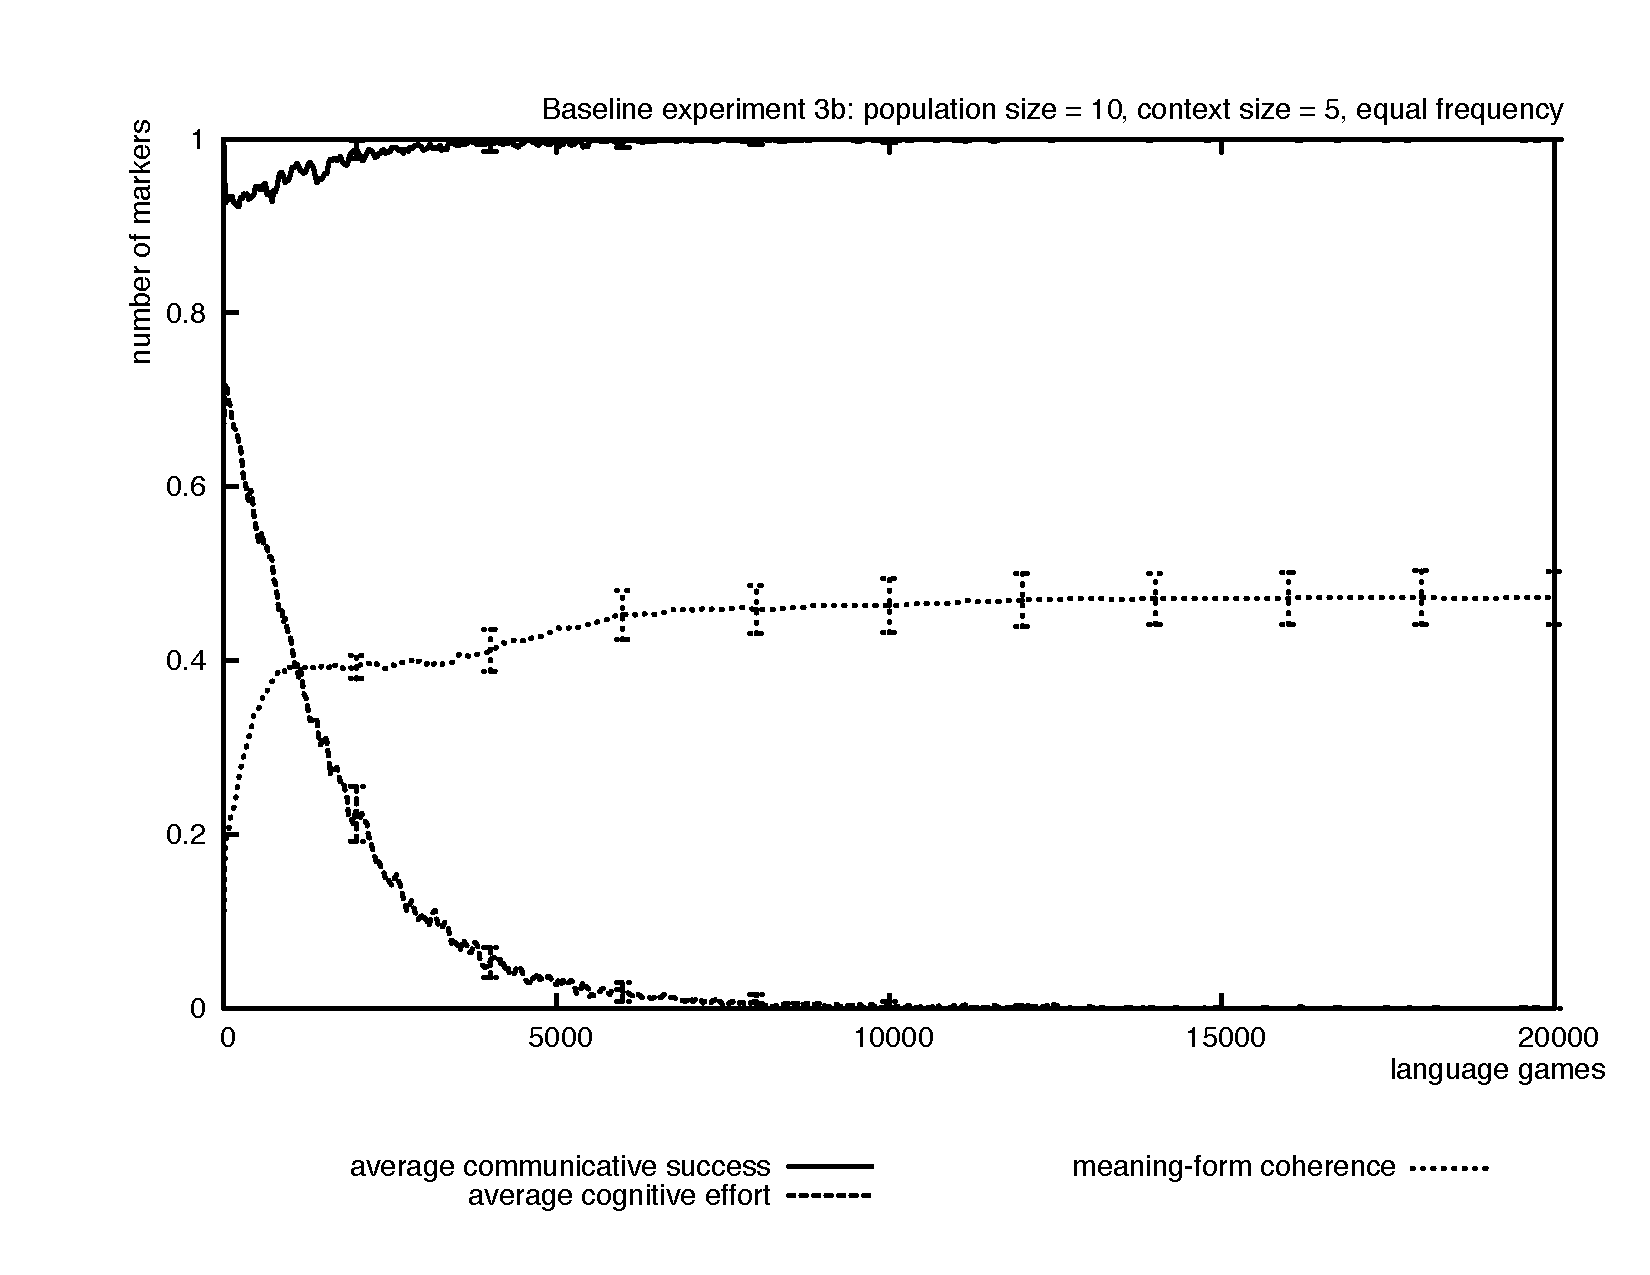
\includegraphics[width=\textwidth]{Chapter3/figs/graph-base3-effort3b}}
  \caption[Baseline experiment 3b: success, effort and coherence]{This graph shows that the agents reach 100\% communicative success\is{communicative success} and reduce the cognitive effort\is{cognitive effort} needed for interpretation. However, the meaning-form coherence only reaches about 40\% which indicates that the agents did not converge on a shared set of marker\is{case!case marking}s but keep using divergent preferences in more than half of the language game\is{language game}s.}
   \label{f:base3-effort3b}
\end{figure}


\subsubsection{Discussion}
 The results of baseline experiment 3b seem to be contradictory at first sight: even though the agents do not agree an a shared preferred set of marker\is{case!case marking}s, they nevertheless reach communicative success\is{communicative success}. This is possible because success in communication does not require meaning-form coherence: if the agents learn all the variation\is{variation}s floating around in the population\is{speech population}, they can still parse all utterances correctly. This happens indeed in this experiment.

The lack of convergence on a preferred set of marker\is{case!case marking}s clearly indicates that the proposed alignment strateg\is{alignment strategy}y is insufficient. The reason is that the alignment strateg\is{alignment strategy}y in which each item has its own single confidence\is{confidence} score is best suited for simulations in which there is always a {\em one-to-one} mapping between form and meaning (as was the case in baseline experiment 2). However, when marker\is{case!case marking}s get generalized to cover more than one participant role\is{participant role}, they become polysemous {\em one-to-more} mappings.

I will go through an example to explain why the single confidence\is{confidence} score cannot be sufficient for polysemous form-meaning mappings. Suppose that an agent knows three marker\is{case!case marking}s: {\em -ma}, {\em -bo} and {\em -li} and that the first two are generalized to cover two roles each whereas {\em -li} is still a verb\is{verb}-specific marker\is{case!case marking}. For convenience's sake, I will not include all the linguistic items involved but treat the marker\is{case!case marking}s as if they were lexical items:

\ea
\parbox{\textwidth}{
\begin{align*}
\begin{array}{ll} 
\text{<move-inside-1>} & \leftarrow \\
\text{<walk-to-2>} & \leftarrow
\end{array}
& \text{(0.5)}\rightarrow \text{-ma}
\end{align*}
}
\z

\ea
\parbox{\textwidth}{
\begin{align*}
\begin{array}{ll} 
\text{<move-inside-1>} & \leftarrow \\
\text{<move-1>} & \leftarrow
\end{array}
& \text{(0.5)}\rightarrow \text{-bo}
\end{align*}
}
\z

\ea
\parbox{\textwidth}{
\begin{align*}
\begin{array}{ll}
\text{<move-1>}\hspace{1,05cm} & \leftarrow
\end{array}
& \text{(0.5)}\rightarrow \text{-li}
\end{align*}
}
\z

Suppose now that the agent observes the utterance {\em boy -ma move-inside} in which the marker\is{case!case marking} {\em -ma} was successfully used for marking `move-inside-1'. The score for {\em -ma} is thus increased and the score for its competit\is{competition}or {\em -bo} is decreased. The consequences for {\em -bo} are far-reaching, because it is now not only less successful than {\em -ma} for covering `move-inside-1', but also than {\em -li} for marking `move-1':

\ea
\parbox{\textwidth}{
\begin{align*}
\begin{array}{ll} 
\text{<move-inside-1>} & \leftarrow \\
\text{<walk-to-2>} & \leftarrow
\end{array}
& \text{(0.6)}\rightarrow \text{-ma}
\end{align*}
}
\z

\ea
\parbox{\textwidth}{
\begin{align*}
\begin{array}{ll} 
\text{<move-inside-1>} & \leftarrow \\
\text{<move-1>} & \leftarrow
\end{array}
& \text{(0.4)}\rightarrow \text{-bo}
\end{align*}
}
\z

\ea
\parbox{\textwidth}{
\begin{align*}
\begin{array}{ll}
\text{<move-1>}\hspace{1,05cm} & \leftarrow
\end{array}
& \text{(0.5)}\rightarrow \text{-li}
\end{align*}
}
\z

In another game, the same damage can be done for the marker\is{case!case marking} {\em -ma} so {\em -bo} can recover from its score decrease. Generalization thus tends to be harmful for the marker\is{case!case marking}s if only one score is used: the more general a role marker\is{case!case marking} gets, the more competit\is{competition}ors it has and thus the more chances that its score will be decreased. Specific marker\is{case!case marking}s can escape punishment through lateral inhibition\is{lateral inhibition} much more easily. On the other hand, if it has competing marker\is{case!case marking}s which are generalized, they can get punished too even if a different participant role\is{participant role} was involved. Suppose that {\em -bo} was observed for marking `move-inside-1' this time, then not only {\em -ma} is seen as a competit\is{competition}or, but also {\em -li} because it overlaps with {\em -bo} for marking `move-1'.

There is thus a constant push-and-pull effect in which marker\is{case!case marking}s may get cornered by others but then all of a sudden get more successful again. This is the reason why the agents can never converge on a preferred set: the single confidence\is{confidence} score does not allow marker\is{case!case marking}s to be successful in one particular context but unsuccessful in another.

\subsection{Results and discussion of set-up 3c}

\begin{figure}[t]
\centerline{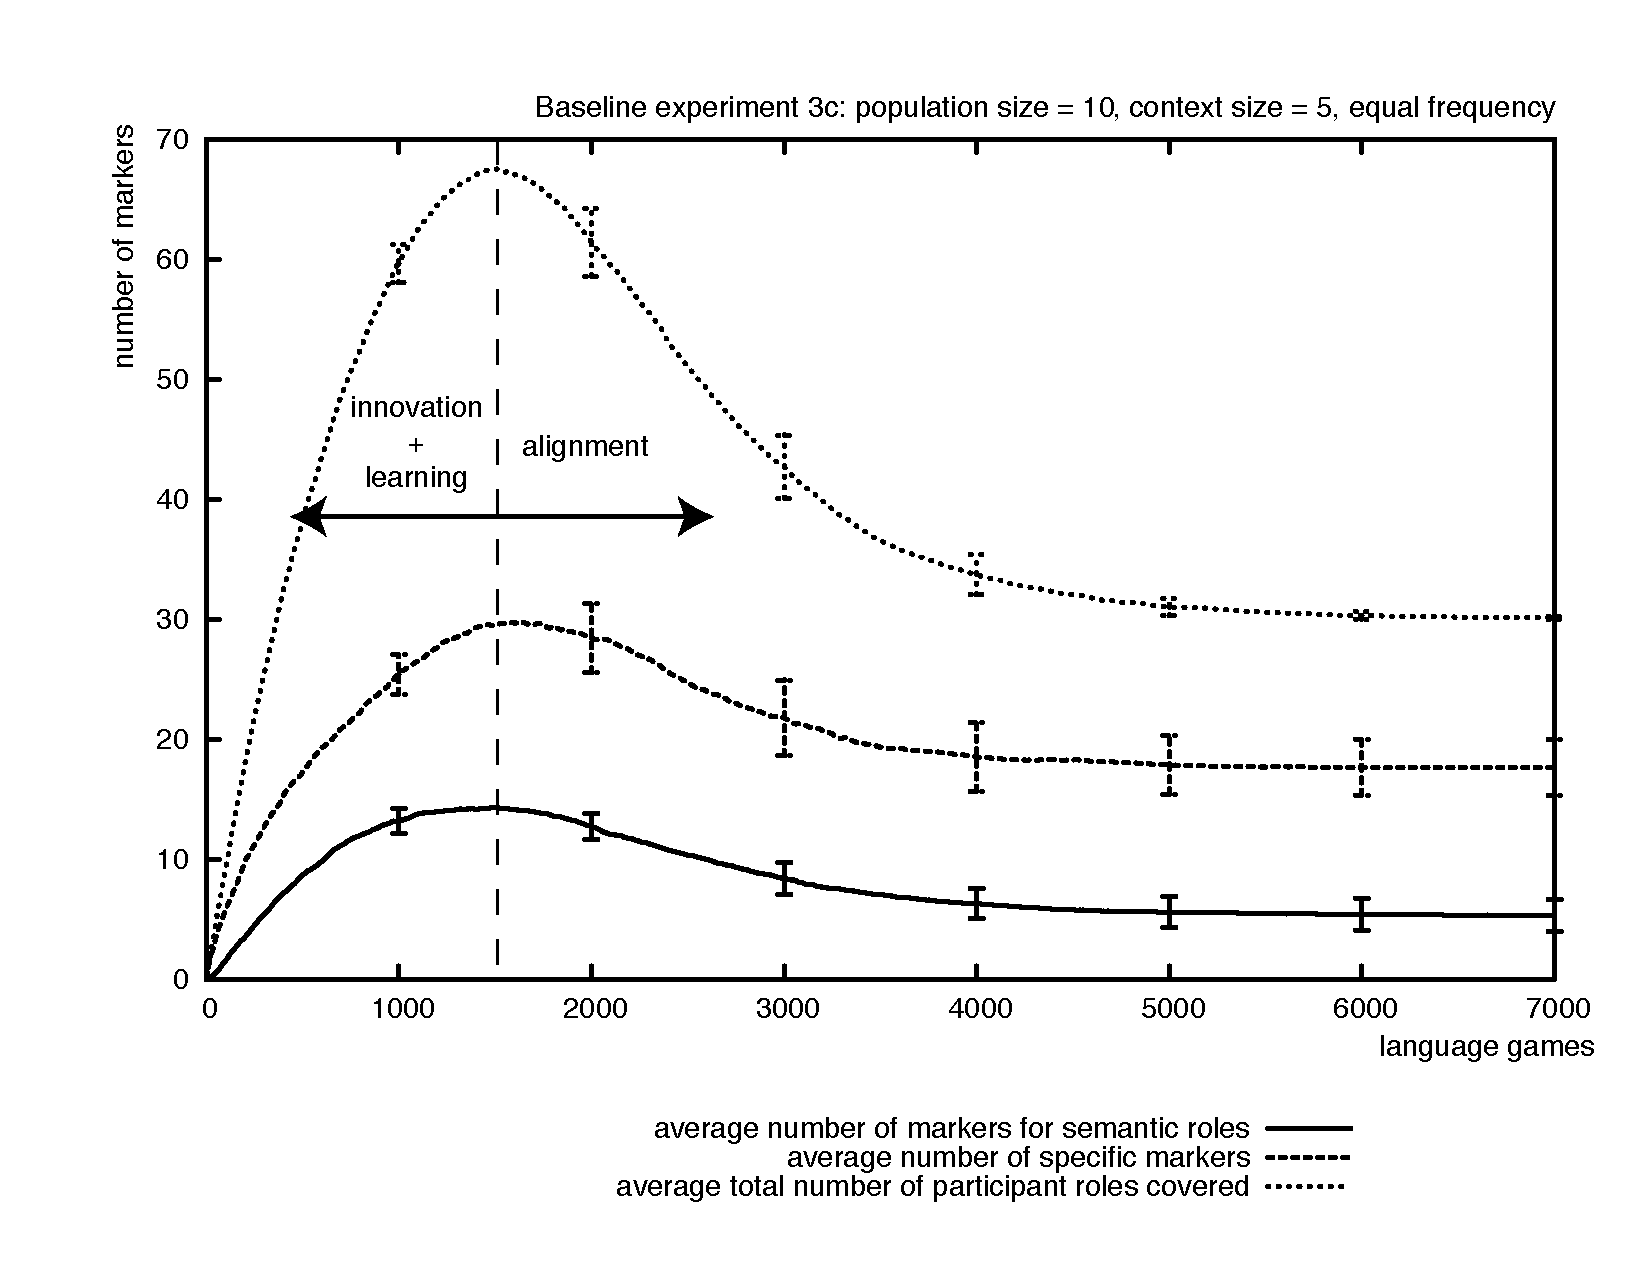
\includegraphics[width=\textwidth]{Chapter3/figs/graph-base3-size3c}}
  \caption[Baseline experiment 3c: number of markers]{The more fine-grained alignment strateg\is{alignment strategy}y allows the agents to converge on one possible marking for each of the thirty participant role\is{participant role}s. There are 5 semantic role\is{semantic role}s on average which each cover about two participant role\is{participant role}s. The remaining 20 roles are covered by specific marker\is{case!case marking}s.}
   \label{f:base3-size3c}
\end{figure}

\begin{figure}[ht]
\centerline{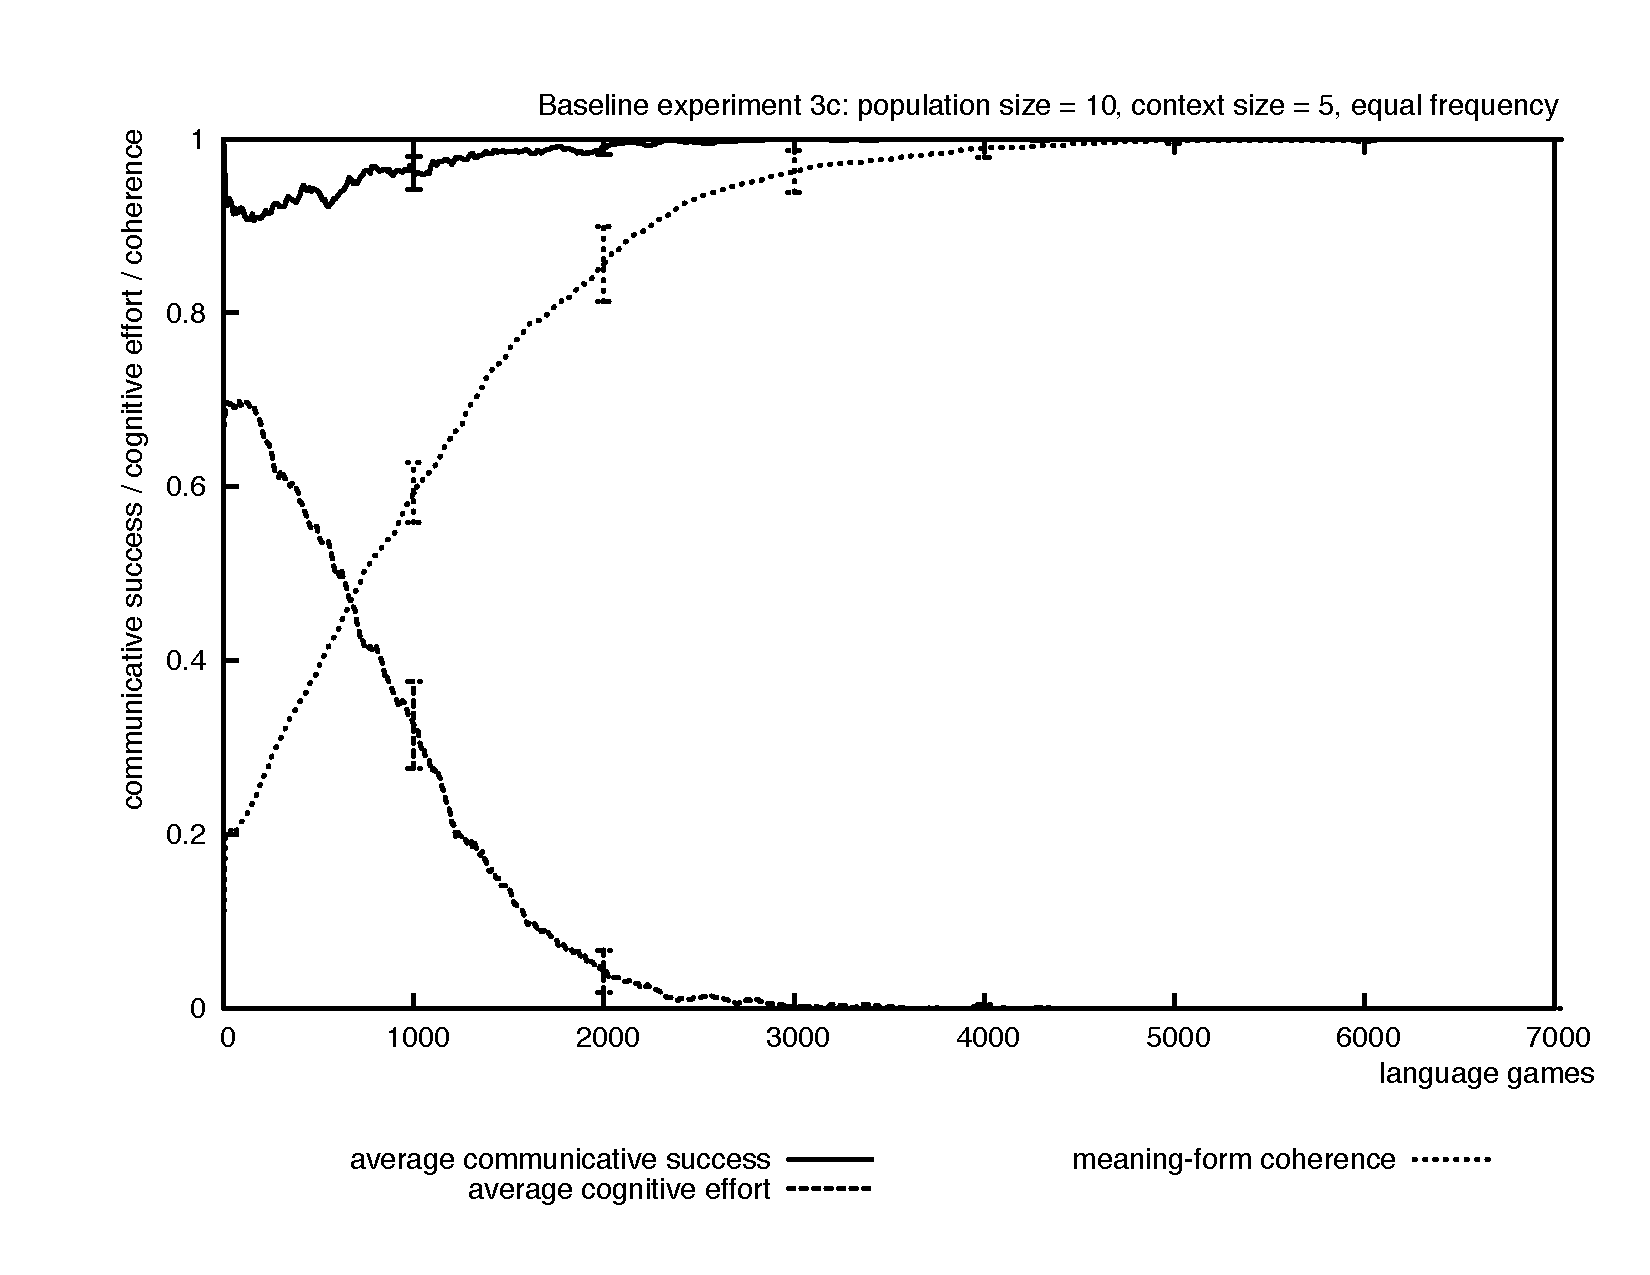
\includegraphics[width=\textwidth]{Chapter3/figs/graph-base3-effort3c}}
  \caption[Baseline experiment 3c: success, effort and coherence]{Using the more fine-grained alignment strateg\is{alignment strategy}y, the agents not only succeed in reaching communicative success\is{communicative success} and reducing cognitive effort\is{cognitive effort}, they also converge on a shared set of meaning-form convention\is{convention}s.}
   \label{f:base3-effort3c}
\end{figure}

\subsubsection{Results}
 The results of baseline experiment 3c indicate that the alignment strateg\is{alignment strategy}y of reinforc\is{reinforcement}ement and lateral inhibition\is{lateral inhibition} can lead to convergence if it is applied in a more fine-grained way. This time, the agents not only use communicative success\is{communicative success} as a guidance but also co-occur\is{co-occurrence}rence links: instead of positing one score on the linguistic item as a whole, they now keep a link between co-occur\is{co-occurrence}ring items and assign a confidence\is{confidence} score to that link. In case of success, the score of the link is increased and only scores of competing {\em links} are decreased. In this model, a marker\is{case!case marking} disappears from the linguistic inventor\is{linguistic inventory}y once it has no links to other linguistic items anymore with a confidencescore higher than zero.

Figure \ref{f:base3-size3c} shows that the number of variation\is{variation}s peaks at 70 possible markings for 30 participant role\is{participant role}s. This means that the agents only have to deal with an average of 2,3 competing marker\is{case!case marking}s for each participant role\is{participant role}. Innovation and adoption of marker\is{case!case marking}s stops at about 1.500 language game\is{language game}s after which the agents rapidly converge on a shared set of marker\is{case!case marking}s. The graph also shows that the agents converge on a set of 5 generalized semantic role\is{semantic role} marker\is{case!case marking}s and about 20 verb\is{verb}-specific marker\is{case!case marking}s. This means that the verb\is{verb}-specific marker\is{case!case marking}s managed to win the competit\is{competition}ion more often than generalized marker\is{case!case marking}s and that semantic role\is{semantic role}s on average only cover two participant role\is{participant role}s.

Figure \ref{f:base3-effort3c} shows that fine-grained alignment allows the agents to converge on a shared set of preferences: meaning-form coherence reaches 100\% after 5.000 language game\is{language game}s which corresponds to the moment where the agents have pruned all the variation\is{variation}s down to 30 in Figure \ref{f:base3-size3c}. The agents also reach communicative success\is{communicative success} and manage to reduce the cognitive effort\is{cognitive effort} needed during parsing.


\subsubsection{Discussion}
 The results show that the fine-grained scoring mechanism suffices to solve the problem of convergence among the agents. However, the gain in inventory optimization is minimal: the agents end up with an average of 25 marker\is{case!case marking}s for 30 participant role\is{participant role}s. Also the benefits of generalization are on the low side with an average of two participant role\is{participant role}s covered by a semantic role\is{semantic role}.

By solving the problem of the single confidence\is{confidence} scores, the fine-grained scoring mechanism created a new one: since only competing links are taken into account during consolidation\is{consolidation}, the influence of the frequency\is{frequency} of the entire category is neglected. This means that a verb\is{verb}-specific marker\is{case!case marking} has the same chances of surviving the competit\is{competition}ion as generalized semantic role\is{semantic role} marker\is{case!case marking}s do, even though the latter ones are as a whole more frequent and productive. If a semantic role\is{semantic role} loses the competit\is{competition}ion from a specific marker\is{case!case marking}, its type frequency\is{type frequency}\is{frequency} is reduced and hence its productivity\is{productivity}.

To overcome this problem, the agents need another alignment strateg\is{alignment strategy}y which both recognizes the impact of generalized roles and is capable of dealing with the context-sensitive nature of polysemous marker\is{case!case marking}s. Experiment 3d implements such a strategy.

\subsection{Results and discussion of set-up 3d}

\begin{figure}[ht]
\centerline{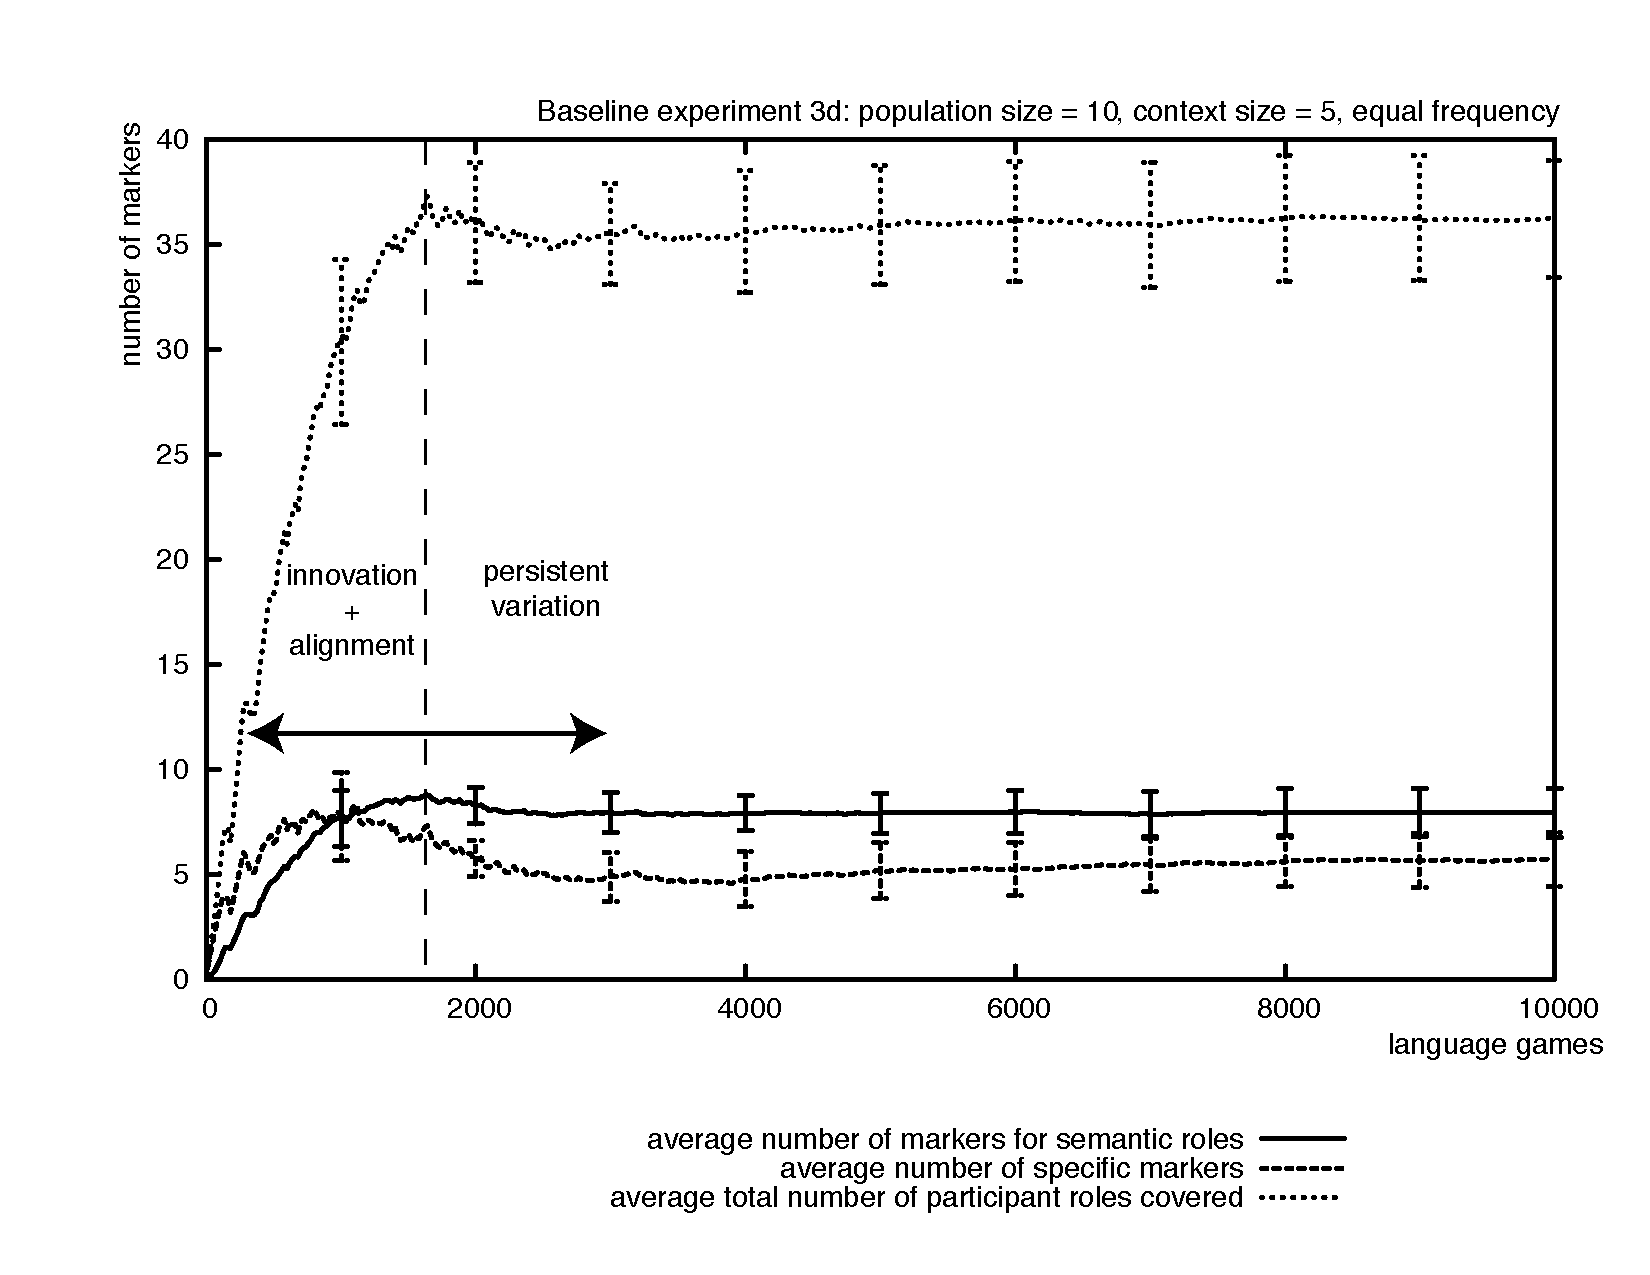
\includegraphics[width=\textwidth]{Chapter3/figs/graph-base3-success3d}}
  \caption[Baseline experiment 3d: number of markers]{When adapting their linguistic behaviours to frequency\is{frequency}, the agents tend to use more generalized semantic role\is{semantic role} marker\is{case!case marking}s rather than specific ones. Here, about seven semantic role\is{semantic role}s cover 25 of the 30 participant role\is{participant role}s. The top line indicates that some amount of variation\is{variation} persists over time.}
   \label{f:base3-size3d}
\end{figure}

\begin{figure}[ht]
\centerline{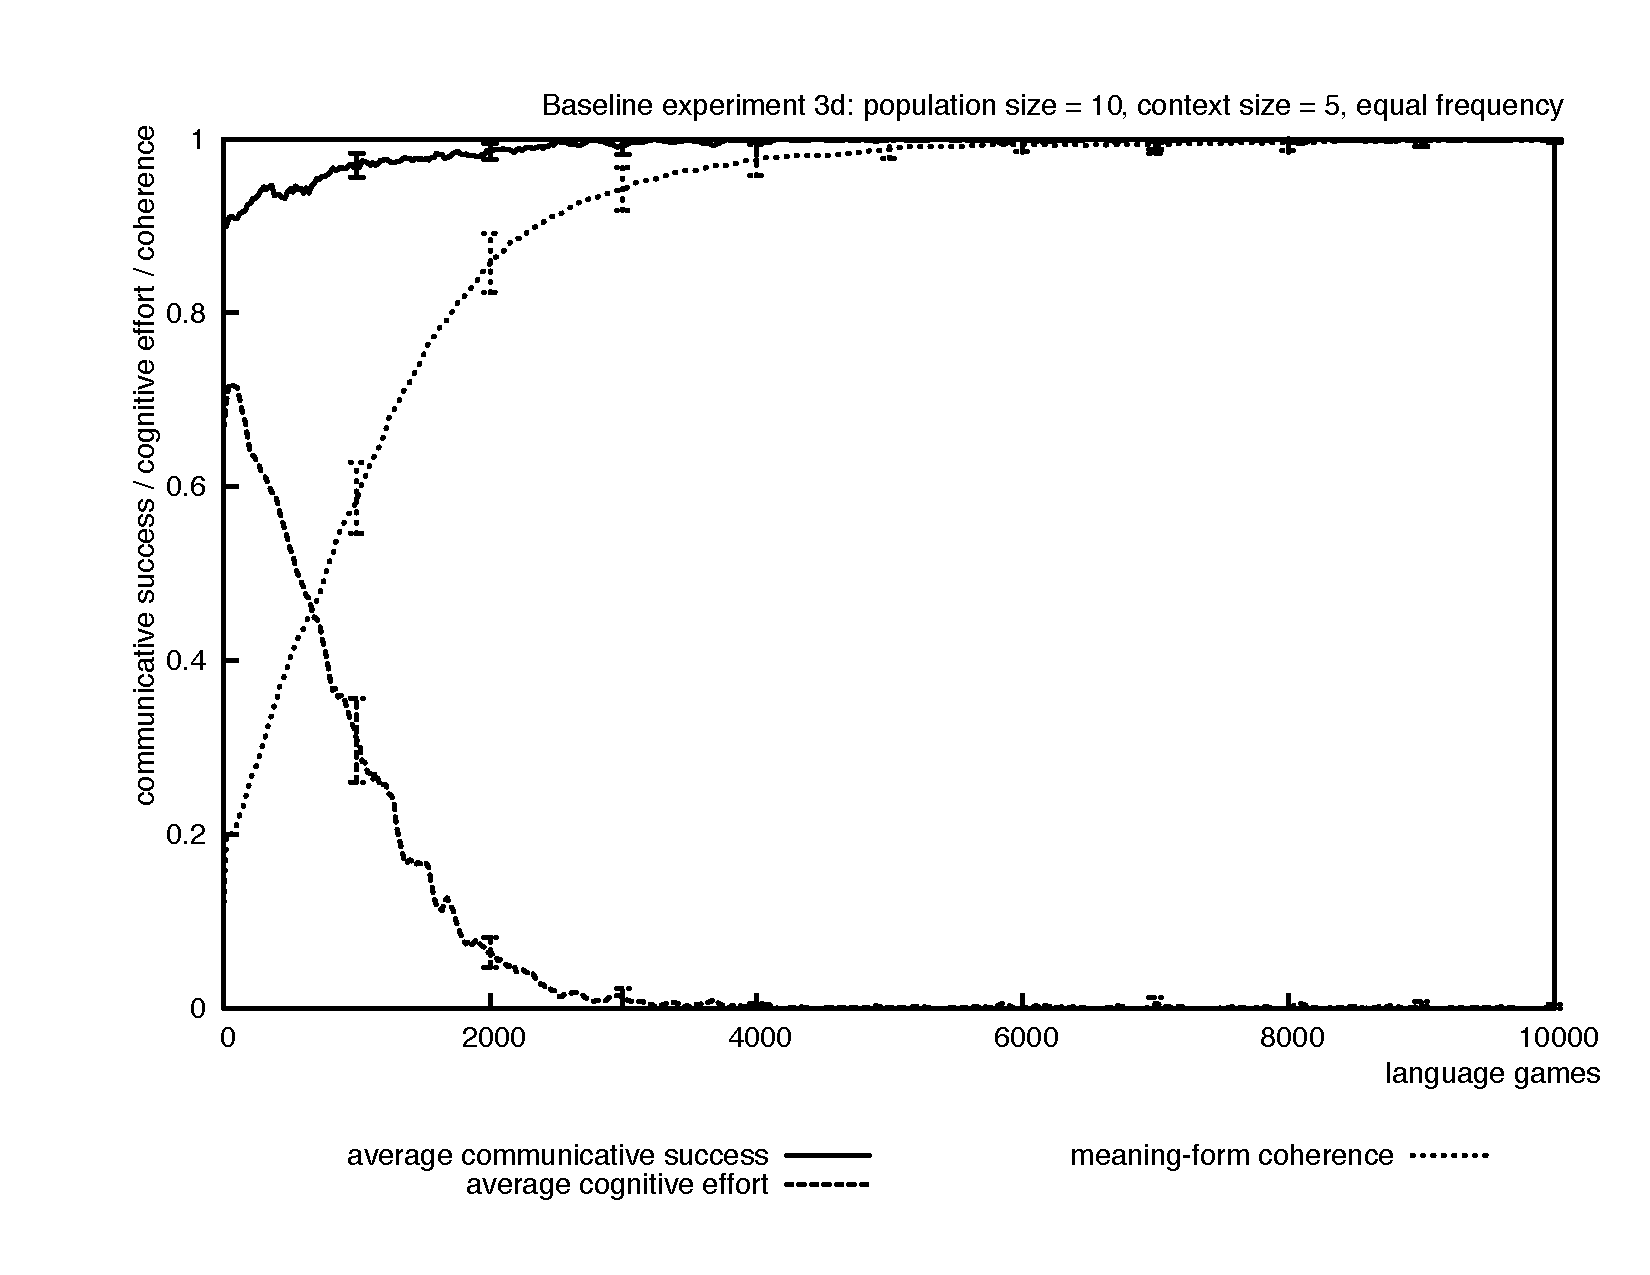
\includegraphics[width=\textwidth]{Chapter3/figs/graph-base3-effort3d}}
  \caption[Baseline experiment 3d: success, effort and coherence]{This graph shows that the agents reach communicative success\is{communicative success}, reduce the cognitive effort\is{cognitive effort} needed for interpretation and converge on a shared set of case marker\is{case!case marking}s.}
   \label{f:base3-effort3d}
\end{figure}

\subsubsection{Results}
 The final set-up in baseline experiment 3 does not use confidence\is{confidence} scores or lateral inhibition\is{lateral inhibition}. Instead, agents rely on token frequency\is{token frequency}\is{frequency} of successful interactions for producing utterances. Figure \ref{f:base3-size3d} shows that the agents spend roughly the same time as in set-up 3c innovat\is{innovation}ing and learning new marker\is{case!case marking}s. The average amount of variation\is{variation} reaches a total of 35--40 possibilities for 30 marker\is{case!case marking}s, which is an average of less than two variation\is{variation}s for each participant role\is{participant role}. The innovat\is{innovation}ion rate is in fact as high as in the previous set-up, but many innovat\is{innovation}ions are excluded very early on by memory decay\is{memory decay}. Innovations that do survive the memory decay\is{memory decay} during the first 2.000 interactions are quite frequent so they persist in memory for a very long time afterwards. Getting rid of them is therefore very slow and may take thousands of additional language game\is{language game}s before they are `forgotten' or in some cases they persist over time. A closer look at the marker\is{case!case marking}s themselves learns us that there are on average eight semantic role\is{semantic role}s and six marker\is{case!case marking}s for specific participant role\is{participant role}s. This means that the semantic role\is{semantic role} marker\is{case!case marking}s can cover up to 24 participant role\is{participant role}s.

Figure \ref{f:base3-effort3d} indicates that even though the agents do not reduce their grammars to a single variation\is{variation} for all 30 participants, they nevertheless converge on a shared set of preferred markings: coherence rises to 100\% in 6.000 language game\is{language game}s. Communicative success\is{communicative success} reaches 100\% and the agents rapidly succeed in reducing the cognitive effort\is{cognitive effort} needed for interpretation. 


\subsubsection{Discussion}
 In order to interpret the results of set-up 3d correctly, a closer examination of the artificial languages of the agents is needed. In one of the simulations, a population\is{speech population} of ten agents all preferred the following 14 marker\is{case!case marking}s and their corresponding participant role\is{participant role}s:

\begin{itemize}
\item {\em -zoti}: cause-move-on-1
\item {\em -ruko}: cause-move-on-2
\item {\em -jaexi}: grasp-2
\item {\em -mad}: approach-1
\item {\em -zima}: give-1
\item {\em -wobae}: give-2
\item {\em -ha}: take-3
\item {\em -qui}: cause-move-on-3, visible-1
\item {\em -fechui}: touch-2, take-1
\item {\em -kuwae}: touch-1, take-2
\item {\em -yuis}: fall-2, approach-2
\item {\em -pae}: give-3, walk-to-2, move-outside-1
\item {\em -ru}: walk-to-1, distance-decreasing-2, move-1, move-inside-2, hide-2, move-outside-2
\item {\em -gahu}: object-1, move-inside-1, fall-1, distance-decreasing-1, hide-1, grasp-1
\end{itemize}

The above marker\is{case!case marking}s suggest that there were seven specific marker\is{case!case marking}s left and seven semantic role\is{semantic role} marker\is{case!case marking}s. However, the marker\is{case!case marking} {\em - jaexi} can in fact be counted as a semantic role\is{semantic role} because it can also cover the participant role\is{participant role}s `hide-2' and `distance-decreasing-2'. In both cases, however, the marker\is{case!case marking} is in competit\is{competition}ion with {\em -ru} which has both a higher type and token frequency\is{token frequency}\is{frequency}. Similarly, {\em -pae} can also cover `hide-1' but this participant role\is{participant role} is dominated by the frequent role marker\is{case!case marking} {\em -gahu}. This explains why in this simulation there remain 33 possibilities for 30 participant role\is{participant role}s instead of only 30: the marker\is{case!case marking}s {\em -jaexi} and {\em -pae} have found their own `semantic niche' in which they occur frequently enough to avoid memory decay\is{memory decay}. Synchron\is{synchronic}ic variation\is{variation} like this is in fact more realistic than the competit\is{competition}ion dynamics in the previous set-ups since it causes a pool of variation\is{variation} which may trigger future changes in the language: both marker\is{case!case marking}s may disappear after a while or they may exten\is{extension}d their usage and become stronger rivals for the now more successful marker\is{case!case marking}s {\em -ru} and {\em -gahu}.

When comparing the results to the two-agent simulations, set-up 3d improves in terms of generalization: more participant role\is{participant role}s are covered by the same marker\is{case!case marking}. The improvement is however not that big so the simulations do not demonstrate that the collective solution found by larger population\is{speech population}s can avoid the local maxima that two agents encountered in their communicative interactions. In order to fully test this hypothesis, experiments are needed involving a larger and more controlled search space.

The alignment strateg\is{alignment strategy}y however does succeed in favouring the more general roles through function and frequency\is{frequency}: marker\is{case!case marking}s which have a higher type frequency\is{type frequency}\is{frequency} and therefore a wider usage tend to have a higher token frequency\is{token frequency}\is{frequency} as well. This creates the same rich-get-richer\is{rich-get-richer dynamics} dynamics of the strategy involving one score and lateral inhibition\is{lateral inhibition} in baseline experiment 2: the more frequent a marker\is{case!case marking} is, the more likely it will win the competit\is{competition}ion in the future and the more likely it will increase its type frequency\is{type frequency}\is{frequency} as well. At the same time, the alignment strateg\is{alignment strategy}y allows for the same context-sensitivity as the fine-grained scoring mechanism because it does not feature explicit lateral inhibition\is{lateral inhibition} so no categories are unrightfully harmed by it. This allows more lexical marker\is{case!case marking}s to still survive in their (sometimes verb\is{verb}-specific) semantic `niche' if they are frequent enough to survive memory decay\is{memory decay}.

\subsection{Conclusions and future work}

In this section I discussed the various set-ups of baseline experiment 3 and reported on its results. Common to all simulations was the additional cognitive ability of analog\is{analogy}ical reasoning over event structure\is{event structure}s. This cognitive mechanism allowed the agents to reuse\is{reuse} (and generalize) existing marker\is{case!case marking}s in new situations and contexts. By exploiting analog\is{analogy}y, the agents are thus capable of generalizing their grammars beyond the input of previous experiences. generalization is thereby not a goal in itself, but rather a side-effect of the need for optimizing communication in an inferential coding system\is{inferential coding system}.

Four set-ups were implemented and compared to each other. The first set-up successfully replicated the original case experiment and set the baseline for the other three multi-agent simulations. Set-up 3b indicated that a single confidence\is{confidence} score is not a sufficient alignment strateg\is{alignment strategy}y for converging on a shared set of preferred markings: this strategy is optimized for one-to-one mappings but cannot deal with the context-sensitiveness of polysemous one-to-many mappings. An alternative was therefore implemented in set-up 3c in which the agents also exploited the co-occur\is{co-occurrence}rences of linguistic items: this time, a specific link was kept between all co-occur\is{co-occurrence}ring items with a confidence\is{confidence} score for each link. The strategy proved itself sufficient for reaching coherence in the population\is{speech population} but at the cost of generalization. Finally, an alignment strateg\is{alignment strategy}y was proposed based on token frequency\is{token frequency}\is{frequency} and memory decay\is{memory decay}. This strategy led the agents to convergence on a set of preferred markings and improved slightly over the results of the two-agent simulations. The various set-ups are summarized in Table \ref{t:consolidation-comparison}.

In the simulations, analog\is{analogy}y is the source of generalization and increased productivity\is{productivity} of existing marker\is{case!case marking}s. This suggests that (at least for innovat\is{innovation}ion and learning), analog\is{analogy}y can be used as a unified account for both the more `regular' forms in the language and the more `irregular' forms as opposed to rule-based accounts which posit abstract rules and a list of exceptions. In order to exploit the power of analog\is{analogy}y, however, the agents need the right kind of alignment strateg\is{alignment strategy}y that favours the more general categories.

\begin{table}[ht] 
\begin{tabular}{ l  l  l  l }
\lsptoprule
{\bfseries Exp.} & {\bfseries Pop.} & {\bfseries Consolidation\is{consolidation}} & {\bfseries Effect}
\\
\midrule
3a & 2 & store innovat\is{innovation}ions & --
\\
3b & 10 & store innovat\is{innovation}ions & alignment fails
\\ & & + confidence\is{confidence} score on all items & 
\\ & & + lateral inhibition\is{lateral inhibition} & 
\\
3c & 10 & store innovat\is{innovation}ions & alignment succeeds
\\ & & + confidence\is{confidence} score on links & (arbitrary winners)
\\ & & + lateral inhibition\is{lateral inhibition} & 
\\
3d & 10 & store innovat\is{innovation}ions & alignment succeeds
\\ & & + frequency\is{frequency} of constructions & (general roles favoured)
\\ & & + memory decay\is{memory decay} & \\
\lspbottomrule
\end{tabular}

\caption[Baseline experiment 3: four alignment strateg\is{alignment strategy}ies]{This table compares the four alignment strateg\is{alignment strategy}ies implemented in baseline experiment 3. In set-up 3a, no additional alignment strateg\is{alignment strategy}ies were needed since there were only two agents and hence no variation\is{variation} was observed in the population\is{speech population}. Set-up 3b showed that direct competit\is{competition}ion did not yield successful alignment because a confidence\is{confidence} score on each linguistic item cannot deal with polysemous usage of the items. Set-up 3c solved the problem of alignment through a confidence\is{confidence} score on each co-occur\is{co-occurrence}rence link. This strategy however led to equal opportunities for each marker\is{case!case marking} in the population\is{speech population} so unproductive marker\is{case!case marking}s survived as easily as general ones. The final strategy involved the frequency\is{frequency} of construction tokens which favoured more general marker\is{case!case marking}s because they have wider application and are thus more frequent.}
\label{t:consolidation-comparison}
\end{table}


\subsubsection{Analogy all the way}
\is{analogy}
 Evidence from natural languages suggests that analog\is{analogy}y is also responsible for the first innovat\is{innovation}ion by recruiting an existing lexical entr\is{lexical entry}y for a more grammatical use instead of inventing a new marker\is{case!case marking} (see section \ref{s:stage2}). Additional experiments are thus needed in which the innovat\is{innovation}ion strategies of baseline experiments 2 and 3 are combined into one. The recruitment of existing and well-entrench\is{entrenchment}ed lexical entr\is{lexical entry}ies would naturally follow from the same assumption\is{assumption}s that language is an inferential coding system\is{inferential coding system} and that speakers and hearers will exploit whatever resources that are available for solving communicative problems: using a convention\is{convention}alized linguistic unit has the major advantage that it offers the hearer a strong grounding point for inferring the meaning or function of the innovat\is{innovation}ion. In the present experiments, the new marker\is{case!case marking}s do not contain any clues about what their source events were, so this may differ strongly from agent to agent which explains why the hearer can't retrieve the analog\is{analogy}y in all cases. In the abstraction\is{abstraction}s and scaffold\is{scaffold}s of the present set-up, however, this poses no problems.

Implementing a more realistic model of stage 2 in the development of case marker\is{case!case marking}s, however, is not a trivial matter and requires more study on how this happens in natural languages. From the evidence gathered so far (see section \ref{s:stage2}), it seems that the present algorithm for analog\is{analogy}y cannot handle this. The first reason is that the recruited lexical item in serial verb language\is{serial verb}\is{verb} constructions, which are typical sources of case marker\is{case!case marking}s, seems to `fit' naturally in the utterance by for example presupposing the same subject\is{syntactic role!subject} as was demonstrated in example \ref{e:thai} which I repeat here: 

\ea
\gll th\^{a}n c\`{a} bin maa krungth\^{e}ep \\
he will fly come Bangkok \\
\glt `He will fly to Bangkok.' \\
\citep[163]{blake94case}
\z


The present analog\is{analogy}y algorithm already expects a marker\is{case!case marking} and would not know how to deal with the other participant role\is{participant role}s of the recruited verb\is{verb}. The task can involve even three participants in cases where for example {\em give} evolves into a dative\is{case!dative} or recipient\is{semantic role!recipient} marker\is{case!case marking}. The data thus show that next to a more general-purpose algorithm for analog\is{analogy}y, we also need to find solutions for coordination and ellipsis so that the recruited lexical entr\is{lexical entry}y can naturally blend in the utterance. Before we can do this, however, we first need to investigate how the syntactic categories can be formed that have to be coordinated.

A second problem has to do with morphology and phonological reduction\is{phonological reduction}. In the attested examples, the second verb\is{verb} in a serial verb language\is{serial verb}\is{verb} construction is implicitly marked for its more grammatical function because it typically occurs in a non-finite\is{finiteness} or a non-conjugated form. In the experiments, there is no morphology or syntax that could distinguish two verb\is{verb}s from each other so the hearer would have a very hard time at figuring out which verb\is{verb} was meant as the `main verb\is{verb}' and which one was meant as the `marker\is{case!case marking}'. Moreover, the hearer would have no reasons to assume that one of the verb\is{verb}s has been recruited for a new use in the first place. The problem with phonological reduction\is{phonological reduction} is that there is no phonological component in the experiments so recruited lexical items cannot evolve towards a new form which distinguishes them more clearly from their original uses.

Next to work on syntax, coordination and morphology, a dynamic representation of categories and word meanings is needed. First steps have already been taken by \citet{wellens08coping} who investigates how word meanings can become more flexible and therefore change over time. This work however only deals with words for objects so more effort is needed to integrate it with the architecture of the experiments in this book. Another particular issue with the model of Wellens is that it does not allow true polysemy\is{polysemy}: the agents continuously shape the meaning of a lexical entr\is{lexical entry}y but they cannot use the same word in multiple ways. The meanings are therefore still one-to-one mappings between form and meaning, but what the exact content of the `one' meaning is may change over time. Grammaticalization of case marker\is{case!case marking}s, however, requires one-to-many mappings or even many-to-many mappings, so the agents have to be capable of distinguishing between different uses of the same form. I believe that coordination and pattern formation\is{formation}\is{pattern formation} could be a key in solving this issue, as I will explain in more detail in the following Chapter.
